\documentclass[english,11pt]{beamer}

\DeclareMathOperator{\Cov}{Cov}
\DeclareMathOperator{\Var}{Var}
\DeclareMathOperator{\E}{\mathbb{E}}
\DeclareMathOperator{\Proba}{\mathbb{P}}

\newcommand{\Covb}[2]{\ensuremath{\Cov\!\left[#1,#2\right]}}
\newcommand{\Eb}[1]{\ensuremath{\E\!\left[#1\right]}}
\newcommand{\Pb}[1]{\ensuremath{\Proba\!\left[#1\right]}}
\newcommand{\Varb}[1]{\ensuremath{\Var\!\left[#1\right]}}

% norm
\newcommand{\norm}[1]{\| #1 \|}

\newcommand{\indep}{\rotatebox[origin=c]{90}{$\models$}}





\usepackage{mathptmx,amsmath,amssymb,graphicx,bibentry,bbm,babel,ragged2e}

\makeatletter

\newcommand{\noun}[1]{\textsc{#1}}
\newcommand{\jitem}[1]{\item \begin{justify} #1 \end{justify} \vfill{}}
\newcommand{\sframe}[2]{\frame{\frametitle{#1} #2}}

\newenvironment{centercolumns}{\begin{columns}[c]}{\end{columns}}
%\newenvironment{jitem}{\begin{justify}\begin{itemize}}{\end{itemize}\end{justify}}

\usetheme{Warsaw}
\setbeamertemplate{footline}[text line]{}
\setbeamercolor{structure}{fg=purple!50!blue, bg=purple!50!blue}

\setbeamersize{text margin left=15pt,text margin right=15pt}

\setbeamercovered{transparent}


\@ifundefined{showcaptionsetup}{}{%
 \PassOptionsToPackage{caption=false}{subfig}}
\usepackage{subfig}

\usepackage[utf8]{inputenc}
\usepackage[T1]{fontenc}


\usepackage{tikz}


\makeatother

\begin{document}


\title{Caractérisation et modélisation de la co-évolution des réseaux de transport et des territoires}

\author{J.~Raimbault$^{1,2,\ast}$\\
\texttt{juste.raimbault@iscpif.fr}
}


\institute{$^{1}$UMR CNRS 8504 G{\'e}ographie-cit{\'e}s\\
$^{2}$UMR-T IFSTTAR 9403 LVMT
}


\date{Soutenance de Thèse\\\smallskip
Lundi 11 juin 2018
}

\frame{\maketitle}


% 



%%%%%
%% Title
%%%%%

% Presentation, remerciement jury, public
% remercie les rapporteurs pour le travail fourni, pris bonne note des pistes damelioiration et correction suggeree - la version courante inclut une grande partie, sera dans version finale avec suggestion de la soutennace.
%



%%%%%
%% Slide 1
%%%%%


%% 1a
% Je voudrais introduire cette présentation par une illustration concrète, vécue, des questions qui se posent quant aux relations entre réseaux de transport et territoires.
%Le village de Tangjia, intégré au district de Xinwan dans la commune de Zhuhai, Delta de la Rivière des Perles, est parmi les plus anciens de la façade ouest du Delta, une existence avec une certaine importance locale étant documentée au moins jusqu'au 17eme siècle. La trajectoire du système urbain local a subi des transformations considérables. Celui-ci s'est retrouvé englobé dans une plus grande agglomération, et peu accessible dans le contexte actuel de la méga-région urbaine.
% Nous voyons sur ces deux photos la ligne à grande vitesse ouverte il y a à peine deux ans. Un effort de développement considérable
% 
% Modelisation comme instrument de connaissance
% Systeme couples / dynamiques couplees -> pb donnees, laboratoires virtuels.
%
% entree par la pont.
%
% Dans une deuxieme slide : problematique. formalisation en systemes. chacun complexe. couplage complexe. donnees suffisent pas. temps long. dynamiques lentes.
%  -> besoin de la modelisation. d'abord comme moyen (ne pas mentionner tout de suite que objet en lui meme)
% V/T : caracteriser : mais pas suffisant (case studies) : y apllier par la modelisation, permet de repondre plus generalement.
% puis deuxieme objet : carac et modelisation : methodes / modelisations / pratiques de modelisation.
%. A DEUX NIVEAU : POSITIONNEMENT a la fois thematique et methodologique. -> deux objectifs. donc theorie.
% pas simple juste thematique.
%  
% -> A DIFFERENTES ECHELLES DE TEMPS ET DESPACE -> plus couplage entre les deux : ammene le besoin de modelisation.
%
\sframe{Du devenir de l'accessibilité à Tangjia}{

\begin{center}

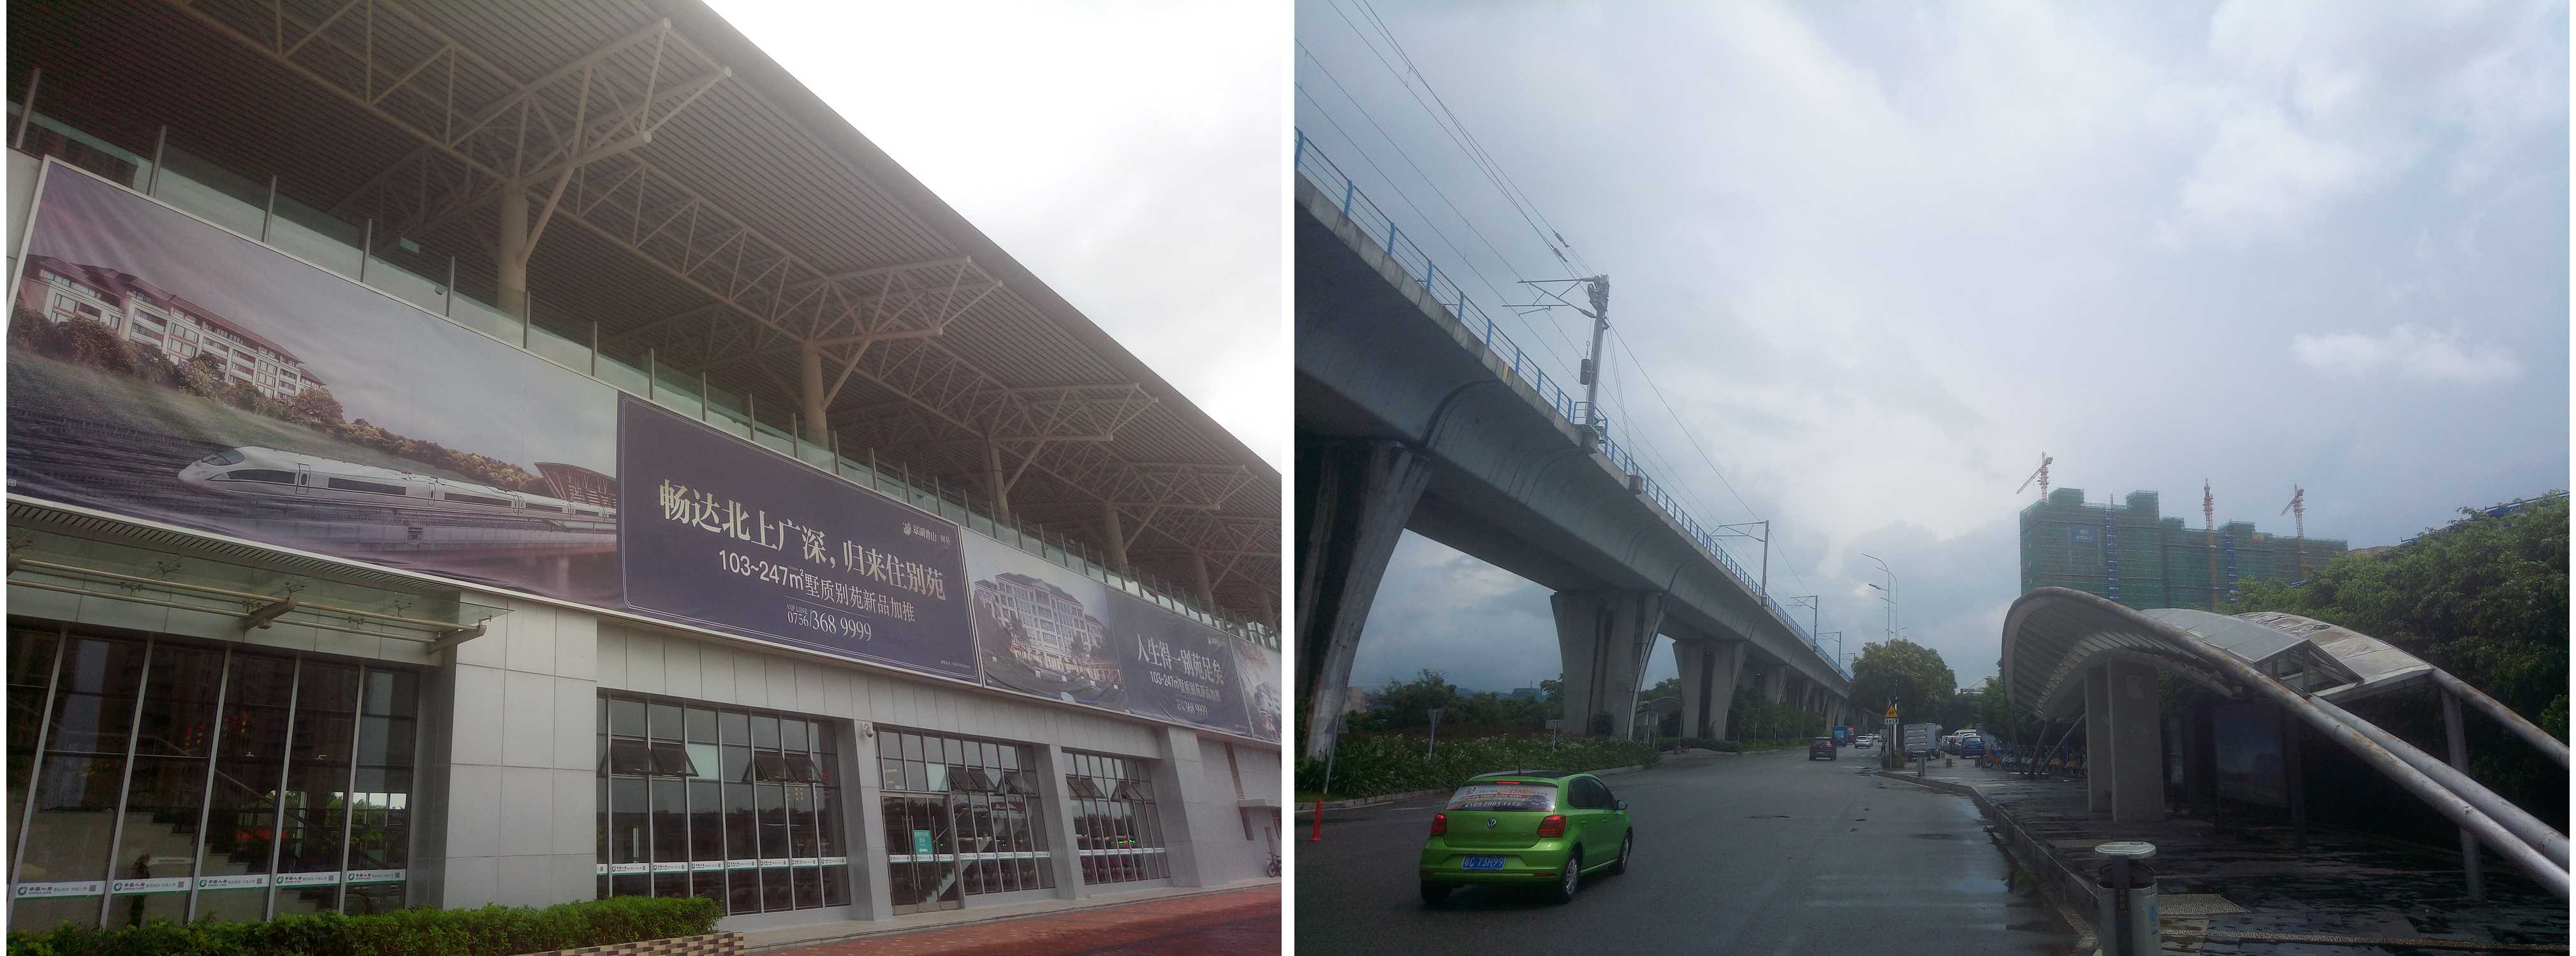
\includegraphics[width=\linewidth]{figures/1-tangjia.jpg}

\end{center}

\medskip

\textit{Pour une approche par la co-évolution}

$\rightarrow$ Réseaux de transport et territoires en co-évolution ? 

$\rightarrow$ Comment caractériser et modéliser celle-ci ?


}

%% 1b
% Nous pouvons d'ores et déjà formuler notre problématique générale et la stratégie adoptée par la thèse.
%\sframe{Pour une approche par la co-évolution}{

% same picture in background, overlay with problematic of the thesis ?
% OR : schema quali.

%$\rightarrow$ Réseaux de transport et territoires en co-évolution ? Comment caractériser et modéliser celle-ci ?

%\bigskip

%\centering

%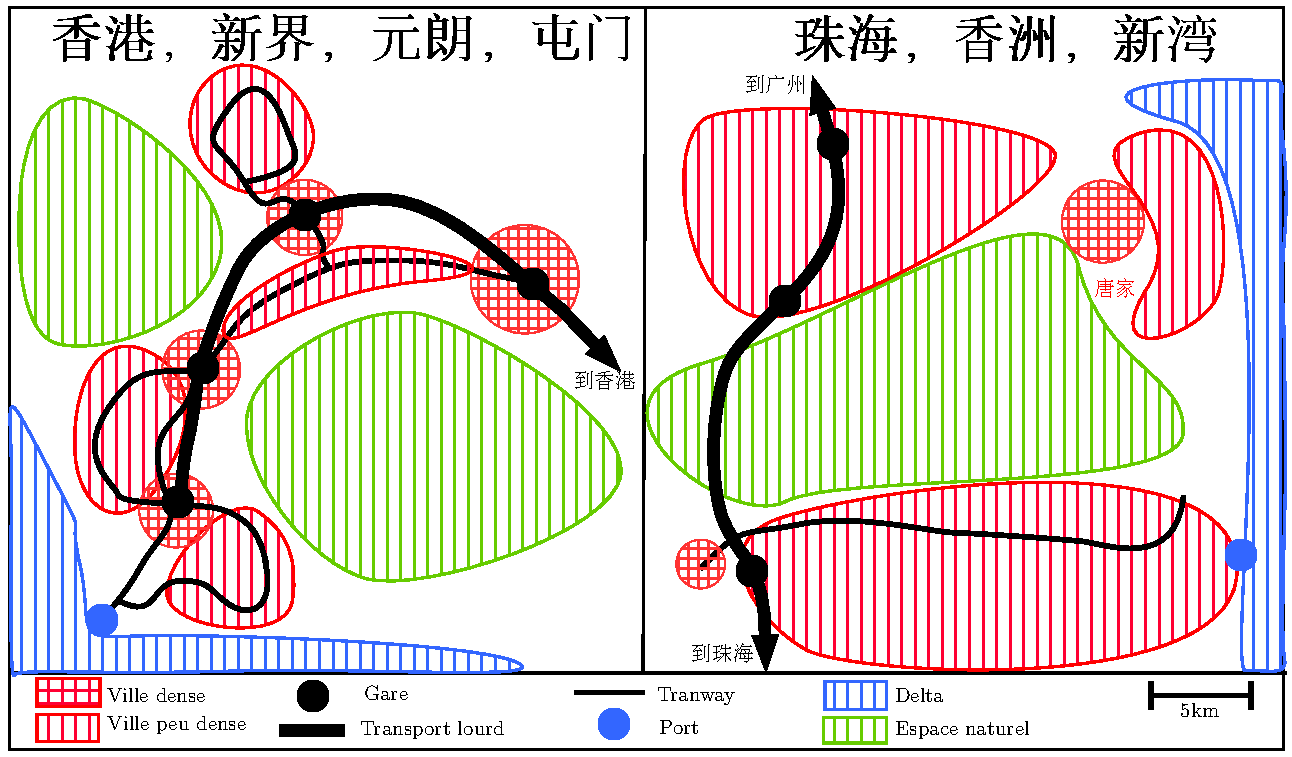
\includegraphics[width=0.8\linewidth]{figures/1-schema.pdf}

%}



%%%%%
%% Slide 2
%%%%%


%% 2
% Il n'est pas ininteressant d'expliciter mon parcours personnel, afin d'éclairer ce choix et positionnements liés à la complexité et methodo-thematique.

% articulation deux domaines de par deux parcours (cf vet)

% Ce parcours est une aventure toujours plus intégrée, vers des modèles toujours plus complexe.
% Bénéficiant initialement d'une formation scientifique multi-disciplinaire,
% Ingenieur generaliste de formation
% au sein de laquelle les incursions dans la complexité étaient déjà inconsciemment présentes comme l'illustre l'implémentation du jeu de la vie en illustration,
% mon affinité pour les système urbains et la rencontre révélatrice avec Paul Bourgine et Kashayar Pakdaman m'a poussé vers la formation interdisciplinaire du Master en Sciences de la Cognition et des Systemes Complexes.
% importance de faire les deux. architectes, Ponts
% 
% variment deux casquettes ? sci complexite et thematique.
% 
% Honnete : inge generaliste. interet sc, systemes urbains : Ponts. Geo : accidents de parcours ? : naturel ?
\sframe{}{

% Un ancrage progressif dans la complexité

\begin{columns}
	\begin{column}{0.6\textwidth}
		\textit{Un parcours original}
		\medskip
		\begin{itemize}
			\item Ingénieur généraliste%Formation scientifique multidisciplinaire
			\item Master Systèmes Complexes
			\item Objet ville: architecture, unbanisme.
			\item Ville, Environnement, Transport % Preciser Ponts
			\item Une transition progressive vers les sciences humaines et la géographie, avec approfondissement du sujet % geocites
		\end{itemize}
		\medskip
		
		Amene la double articulation theorique/thematique.
		
		% expliciter.
		
		%$\rightarrow$ \textit{interdisciplinarité et intégration progressives}
	\end{column}
	\begin{column}{0.5\textwidth}
		\centering
		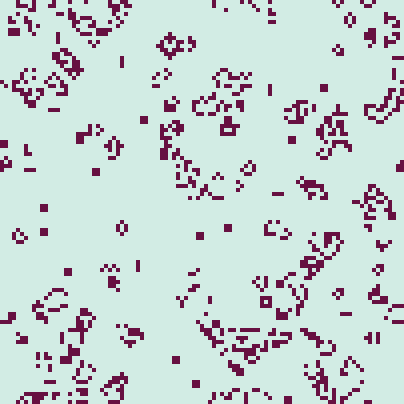
\includegraphics[width=0.4\textwidth]{figures/2_gameoflife.png}\hspace{0.2cm}
		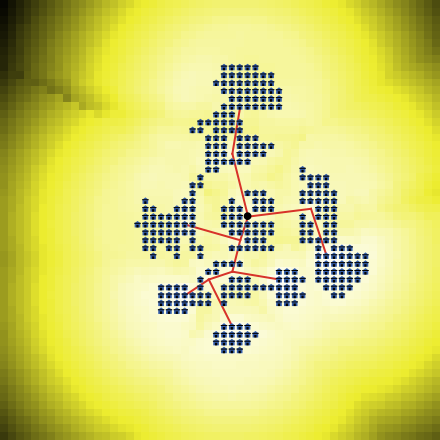
\includegraphics[width=0.4\textwidth]{figures/2_intro_RBD_lattice.png}\\
		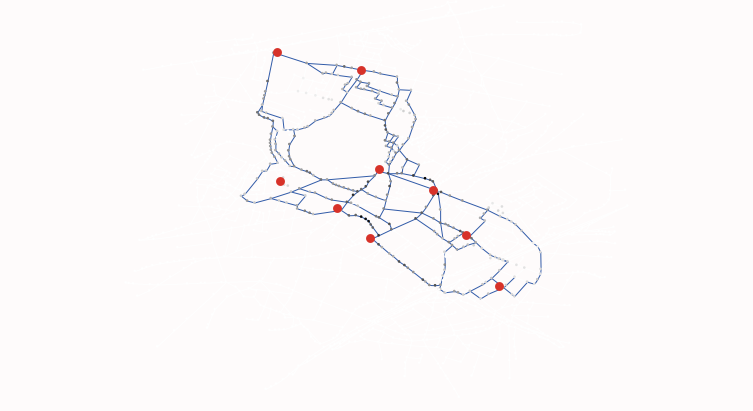
\includegraphics[width=\textwidth]{figures/2_slimemould_reseauFinal.png}\\
		\vspace{-0.5cm}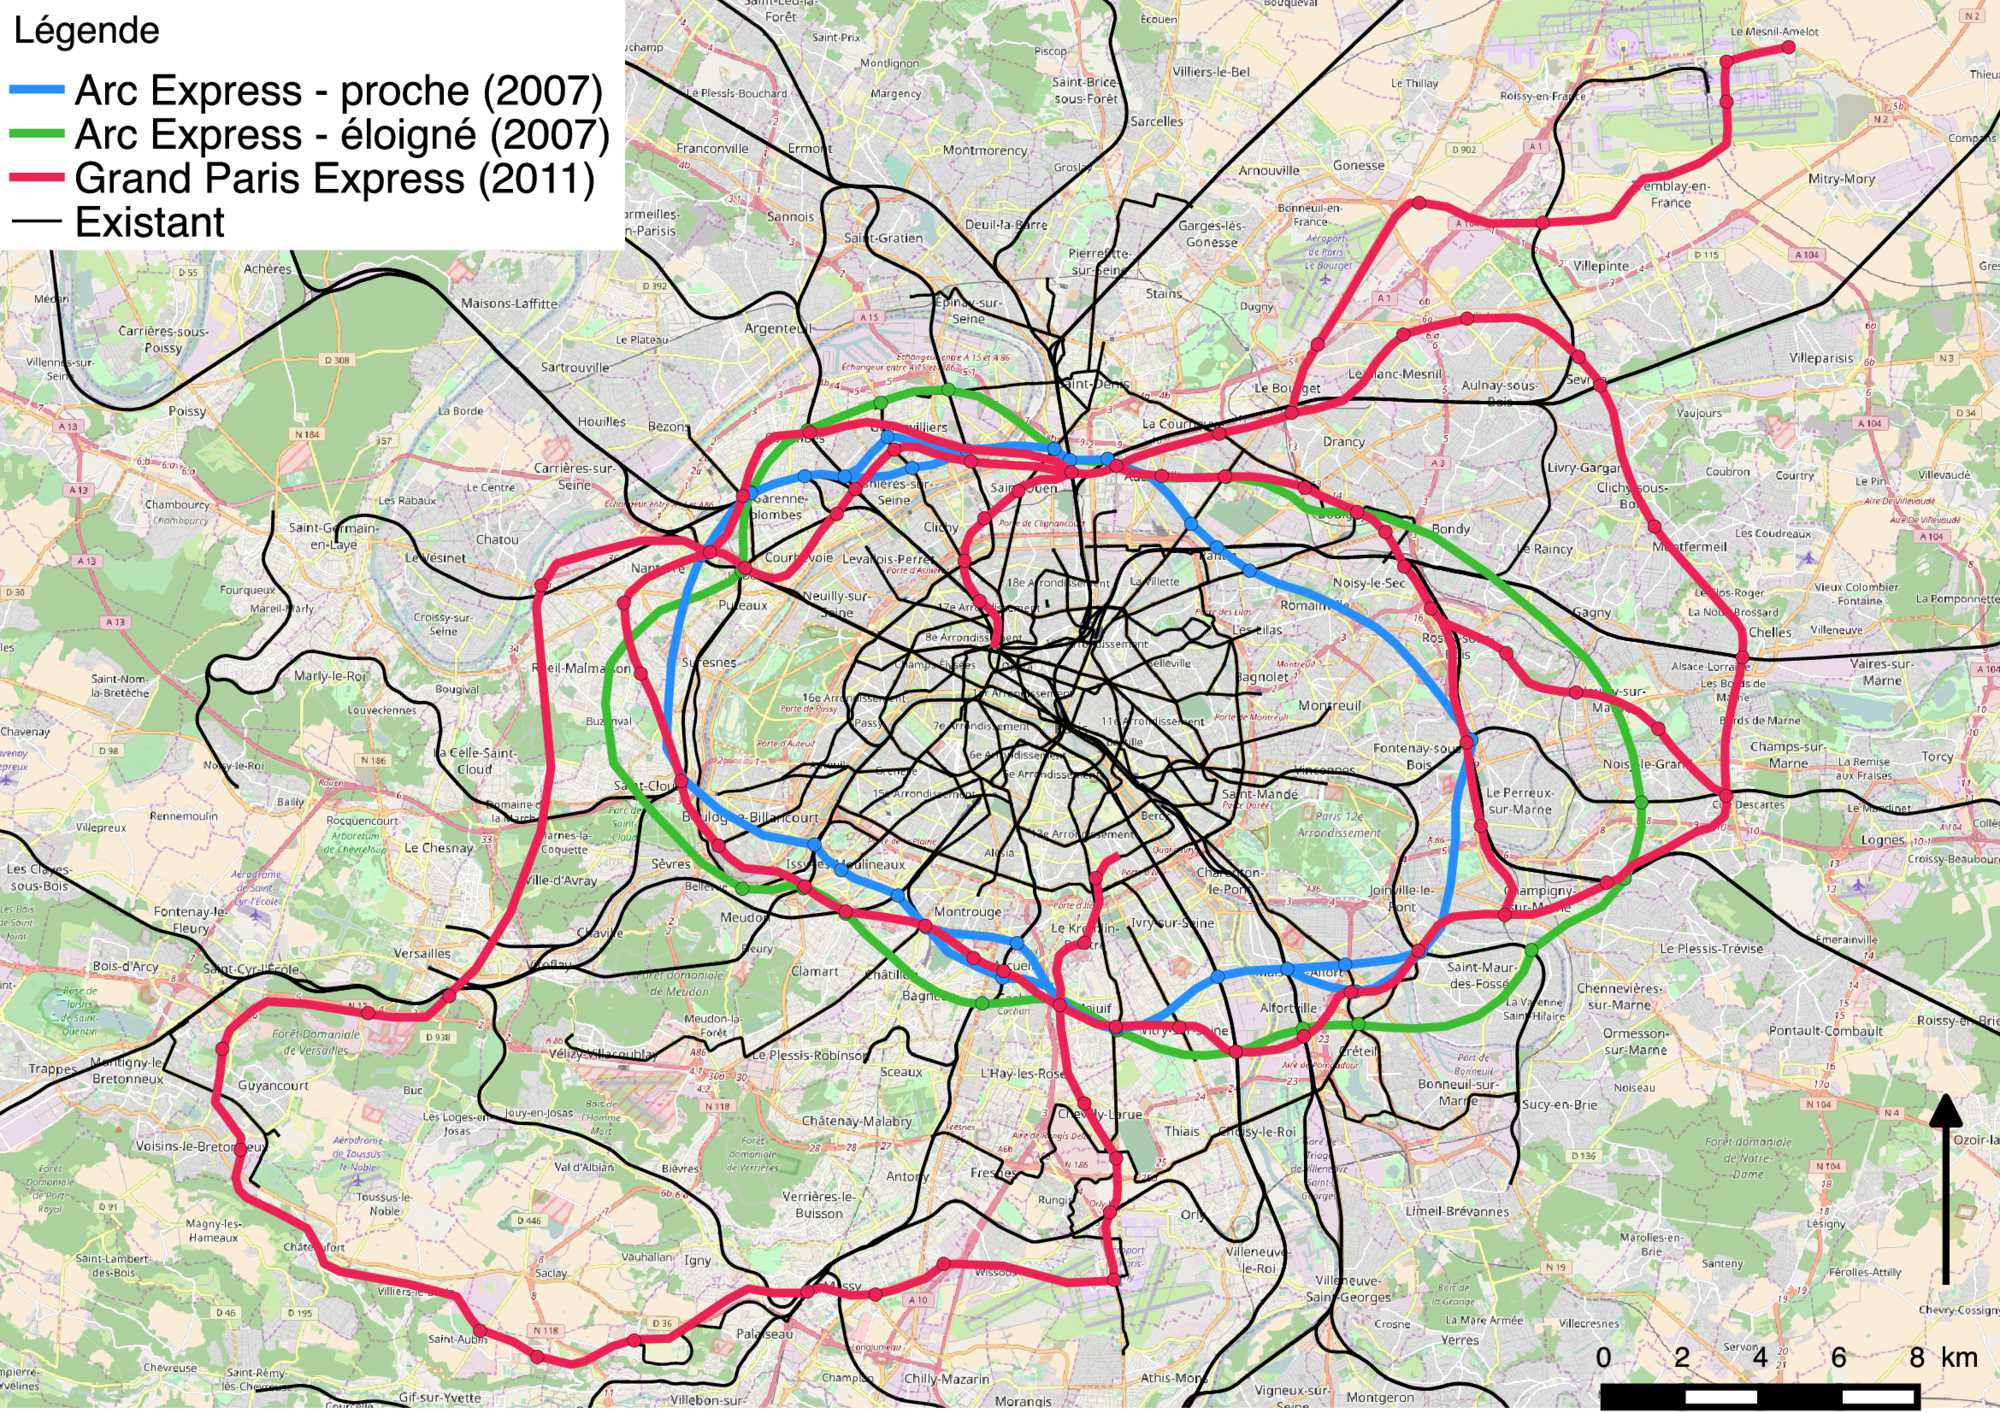
\includegraphics[width=0.8\textwidth]{figures/2-networks.jpg}
	\end{column}
	
\end{columns}

}



%%%%%
%% Slide 6
%%%%%

\sframe{Mise en perspective théorique}{
 
}

%%%%%
%% Slide 7
%%%%%

% 7
% Armés de ces enseignements empiriques et théoriques, nous pouvons tenter une incursion dans la construction de modèles pour comprendre plus finement les processus impliqués
\sframe{Vers une modélisation ? Cartographie des disciplines}{
	
	\vspace{-0.5cm}
	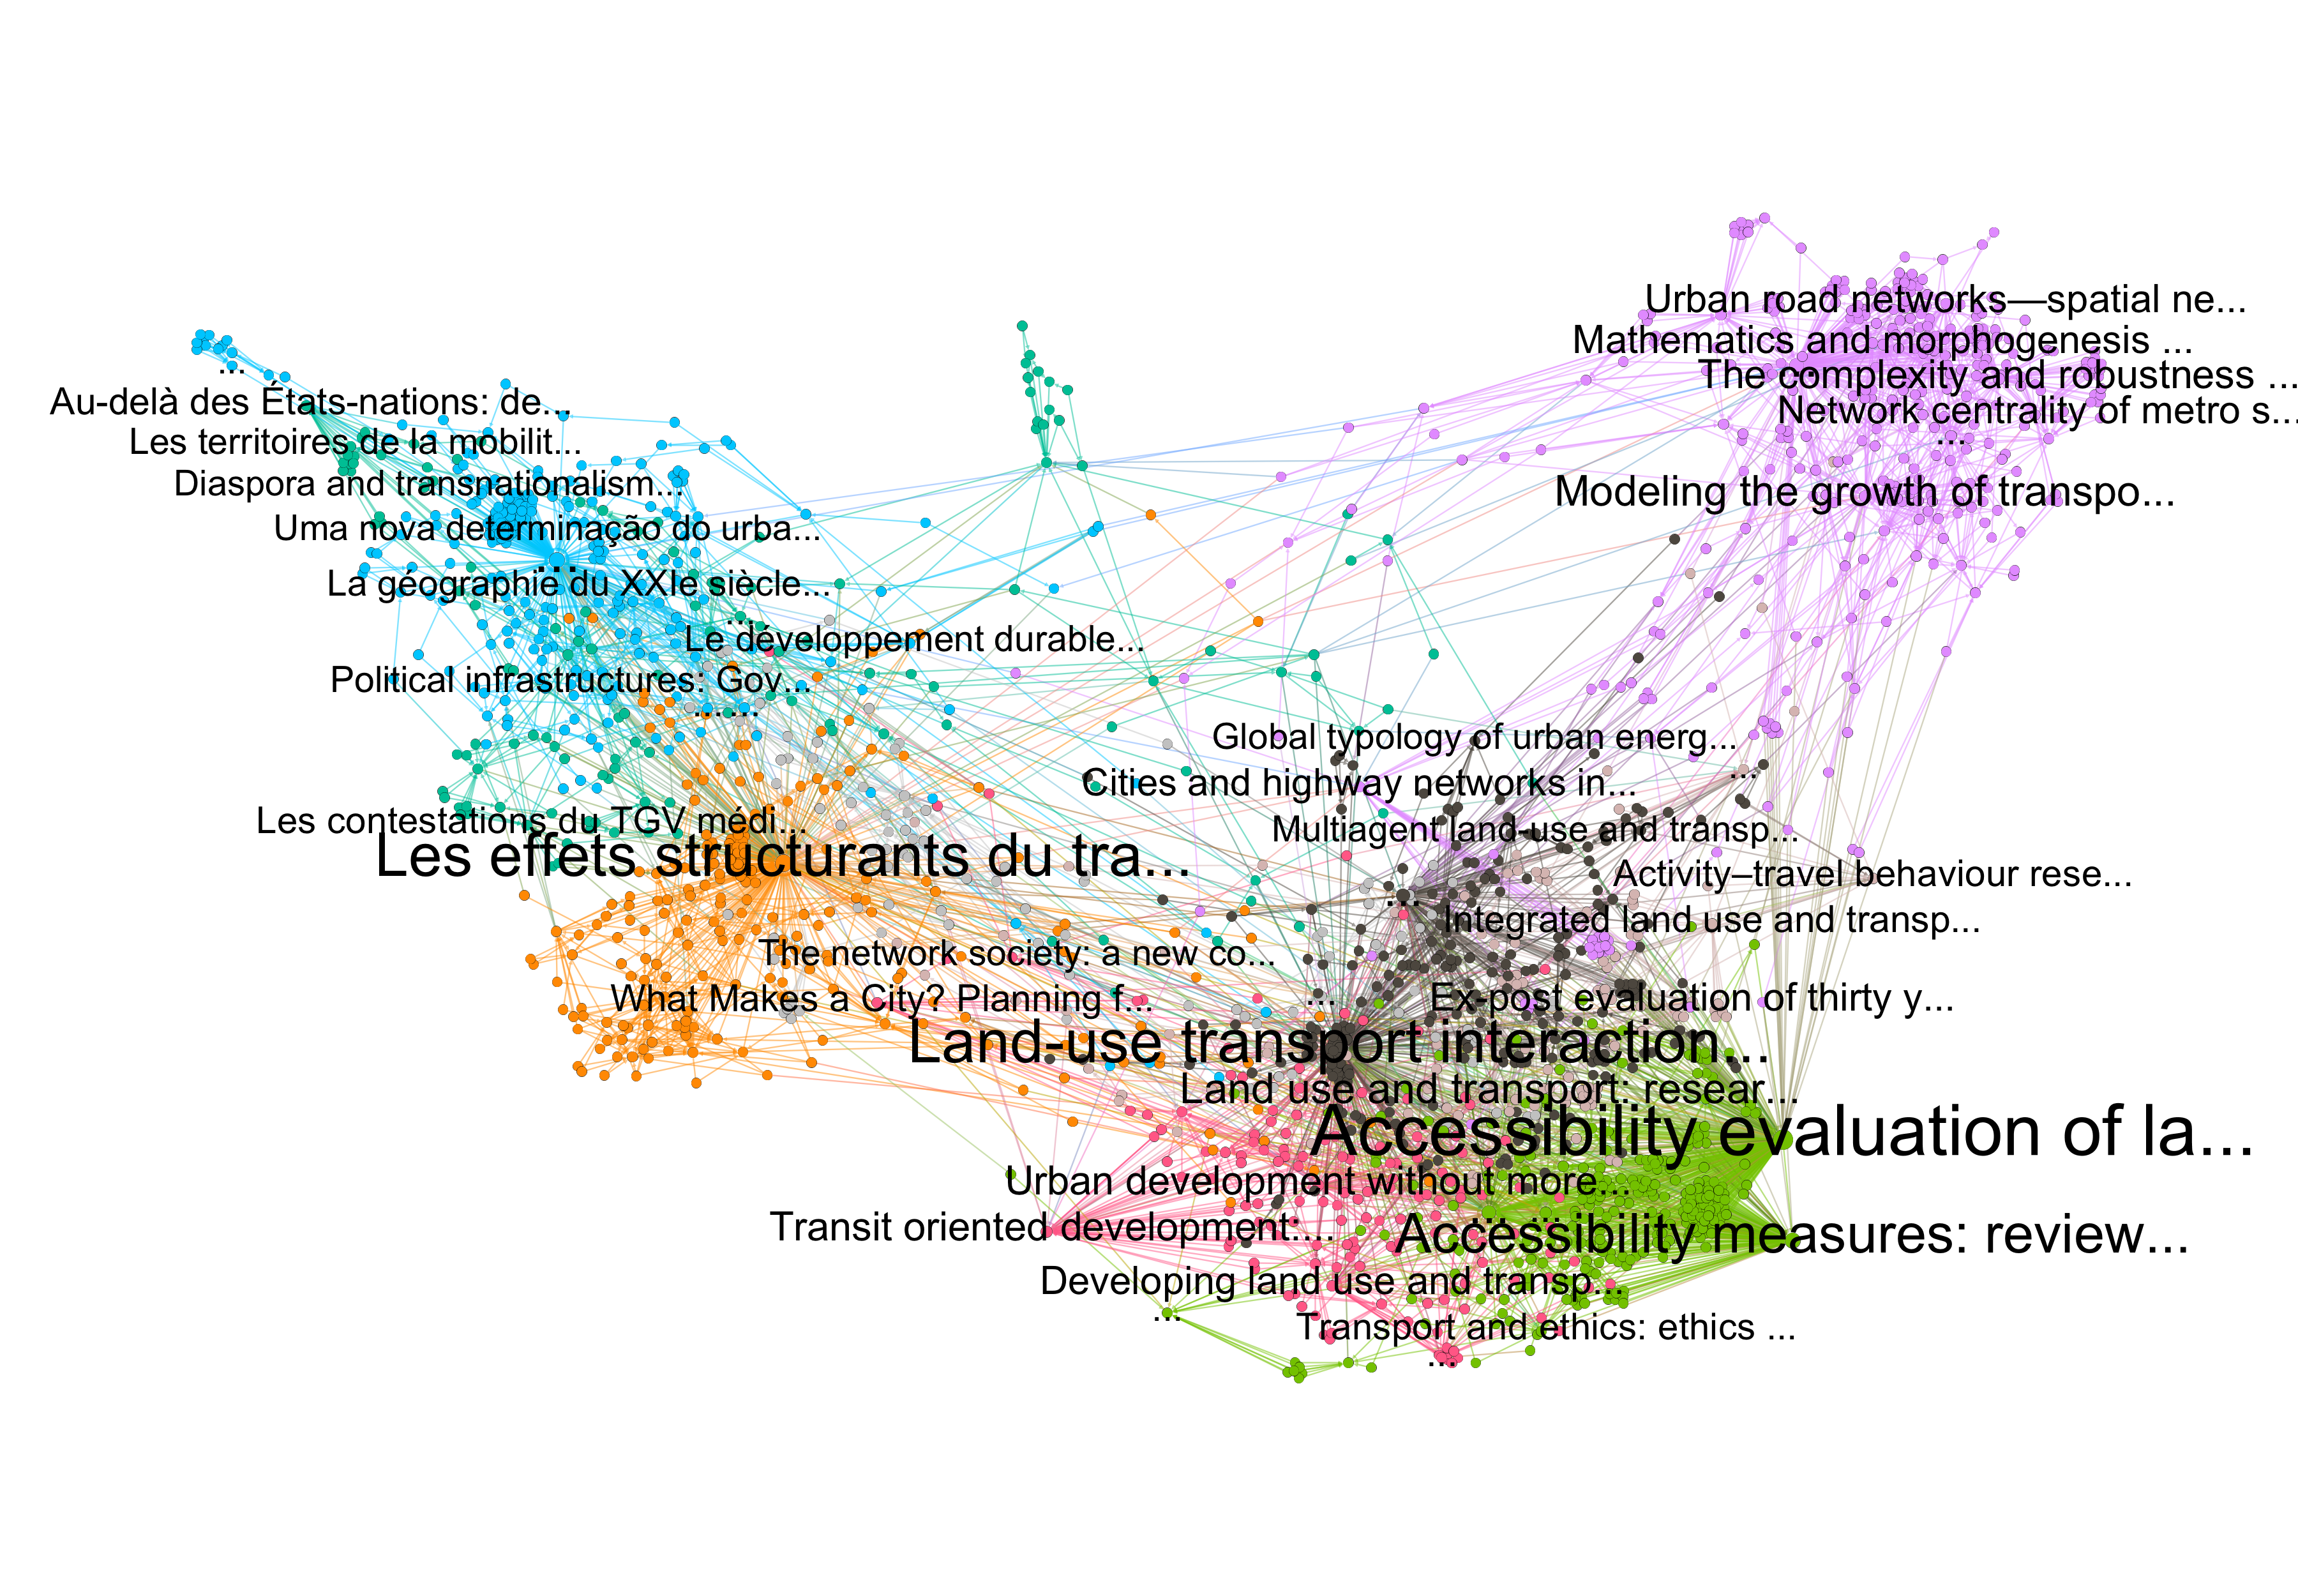
\includegraphics[width=\linewidth]{figures/7-graph.png}
	
	\vspace{-1cm}
	\textit{Multiples points de vue sur les mêmes objets, autant de façons complémentaires de les modéliser.}
}




%%%%%
%% Slide 3
%%%%%


%% 3
%  Cette présentation est l'occasion de suggérer un point de vue original sur le travail effectué. Nous proposons ainsi une entrée non pas linéaire, mais par les différents domaines de connaissance, 
%révélant cette dimension de l'intégration des connaissances.
% Pour mémoire, les domaines de connaissance ont été introduits par (Livet et al., 2010). L'idée est celle d'un va et vient constant entre chacun,
% dans la construction de théories scientifiques complexes,
%avec une place privilégiée

% interesse domaines car deux axes.
\begin{frame}
	\frametitle{Lecture par les domaines de connaissance}
	\begin{center}
	\begin{tikzpicture}
		\node (a) at (0,0) {Empirique}; % visible tout le temps
		\uncover<2->{ % visible à partir du transparent 2
			\node (b) at (3,3) {Théorique};
			\draw[<->] (a) -- (b);
		}

		\uncover<3->{ % visible à partir du transparent 3
			\node (c) at (6,0) {Modélisation};
			\draw[<->] (c) -- (b);
			\draw[<->] (a) -- (c);
		}
	\end{tikzpicture}
	
	\end{center}
	
	\only<4>{
	\vspace{1cm}
	%\textit{Domaines des méthodes, outils et données tout aussi nécessaires dans la construction de perspectives \cite{raimbault2017applied}}
	
	% METTRE DANS LE SCHEMA - apparaitre en deux temps.
	
	}
	
	
\end{frame}


%%%%
%% Transition ?

% carac -> indicateurs.
%  : definir coevol.
%. : differentes formes possibles de relations entre INDICATEURS (pas evident) (systeme toujours via proxys)
%  : comment mettre en relation



%%%%%
%% Slide 4
%%%%%

\sframe{Elaboration d'une méthode de caractérisation}{

\centering

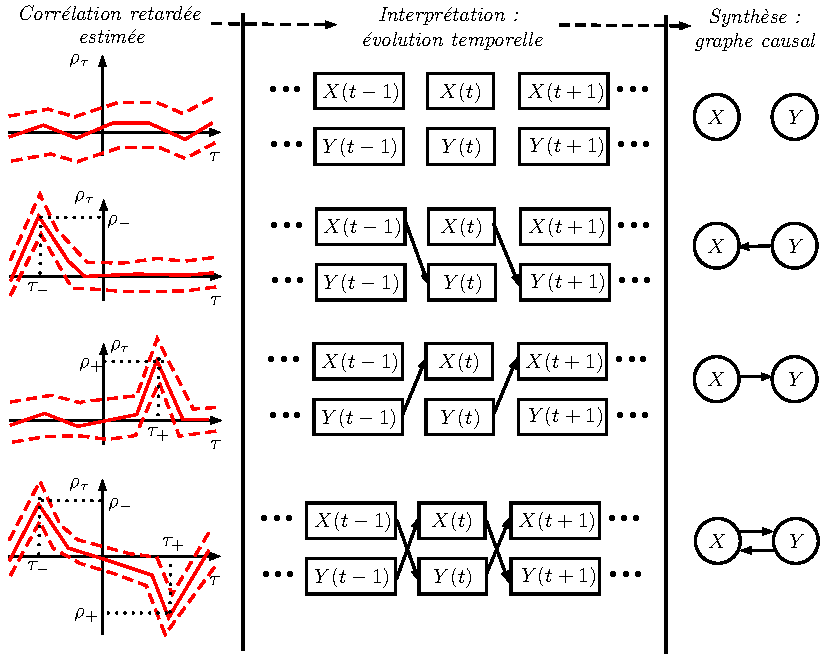
\includegraphics[width=0.9\linewidth]{figures/5-method.pdf}

}


%%%%%
%% Slide 5
%%%%%

% 5
% L'entrée la plus naturelle est celle par les résultat empiriques

\sframe{Des observations empiriques contrastées}{
\begin{columns}
\begin{column}{0.55\textwidth}
	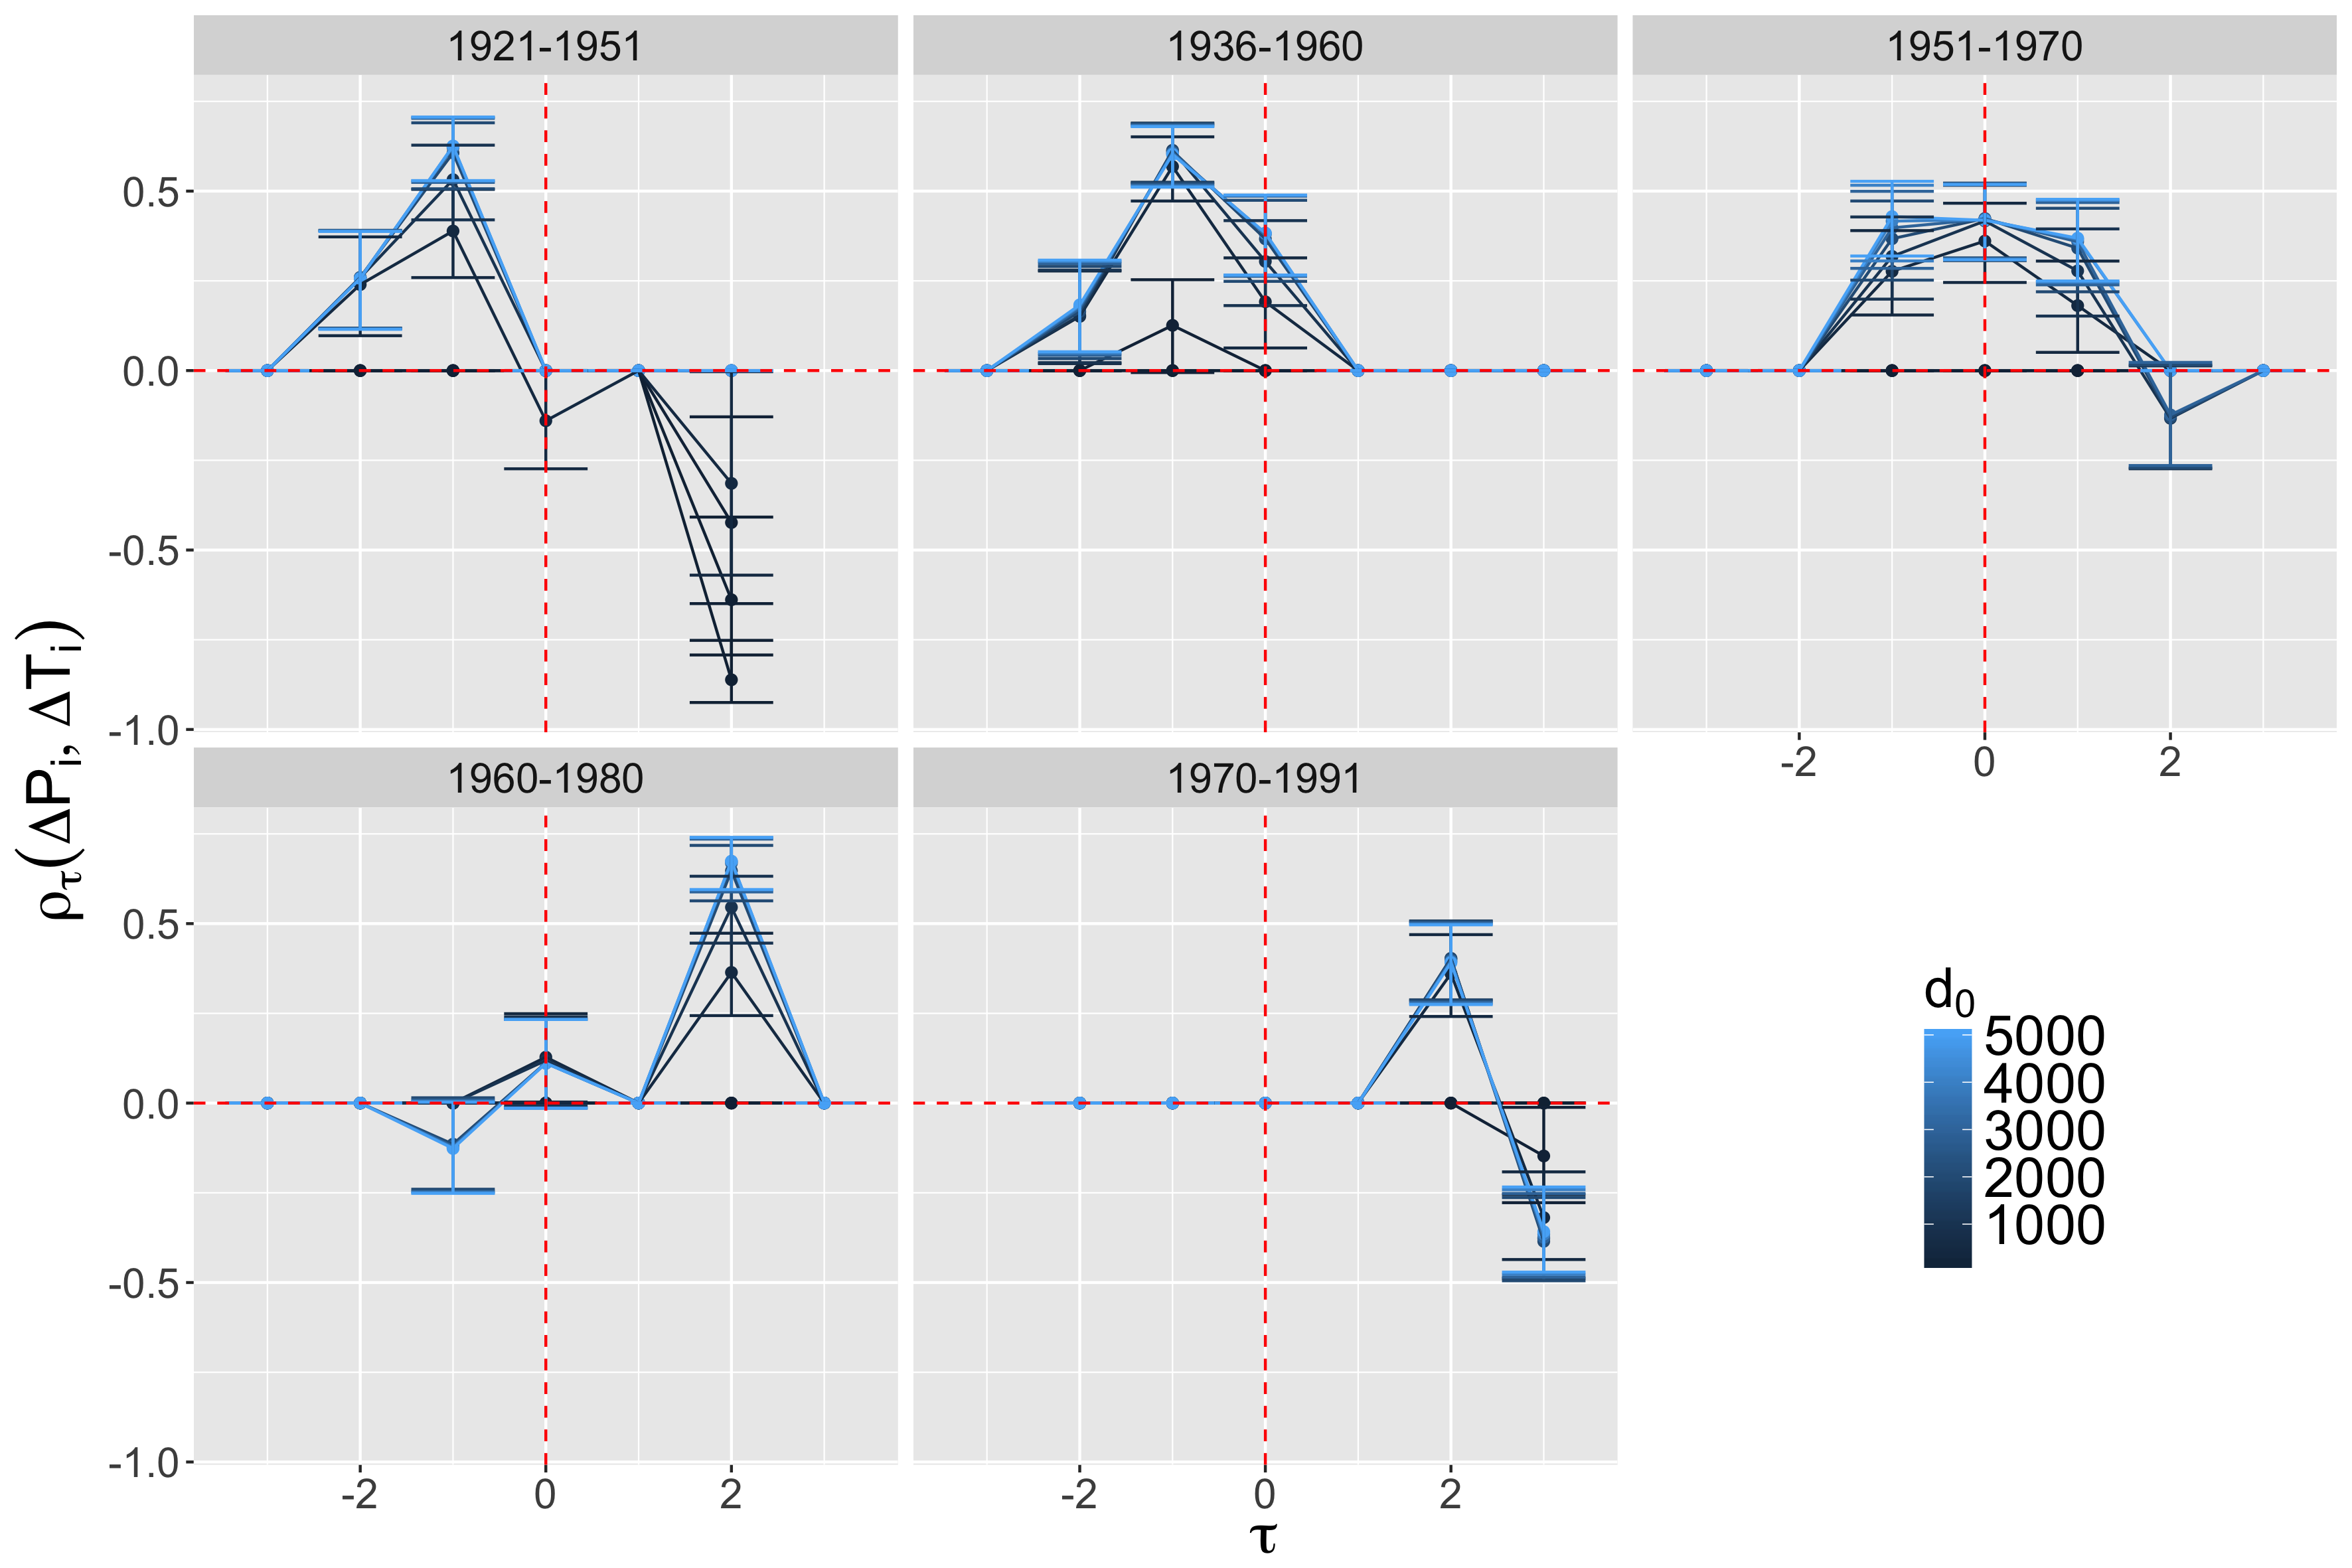
\includegraphics[width=\textwidth]{figures/4-southafrica.png}
\end{column}
	\begin{column}{0.45\textwidth}
	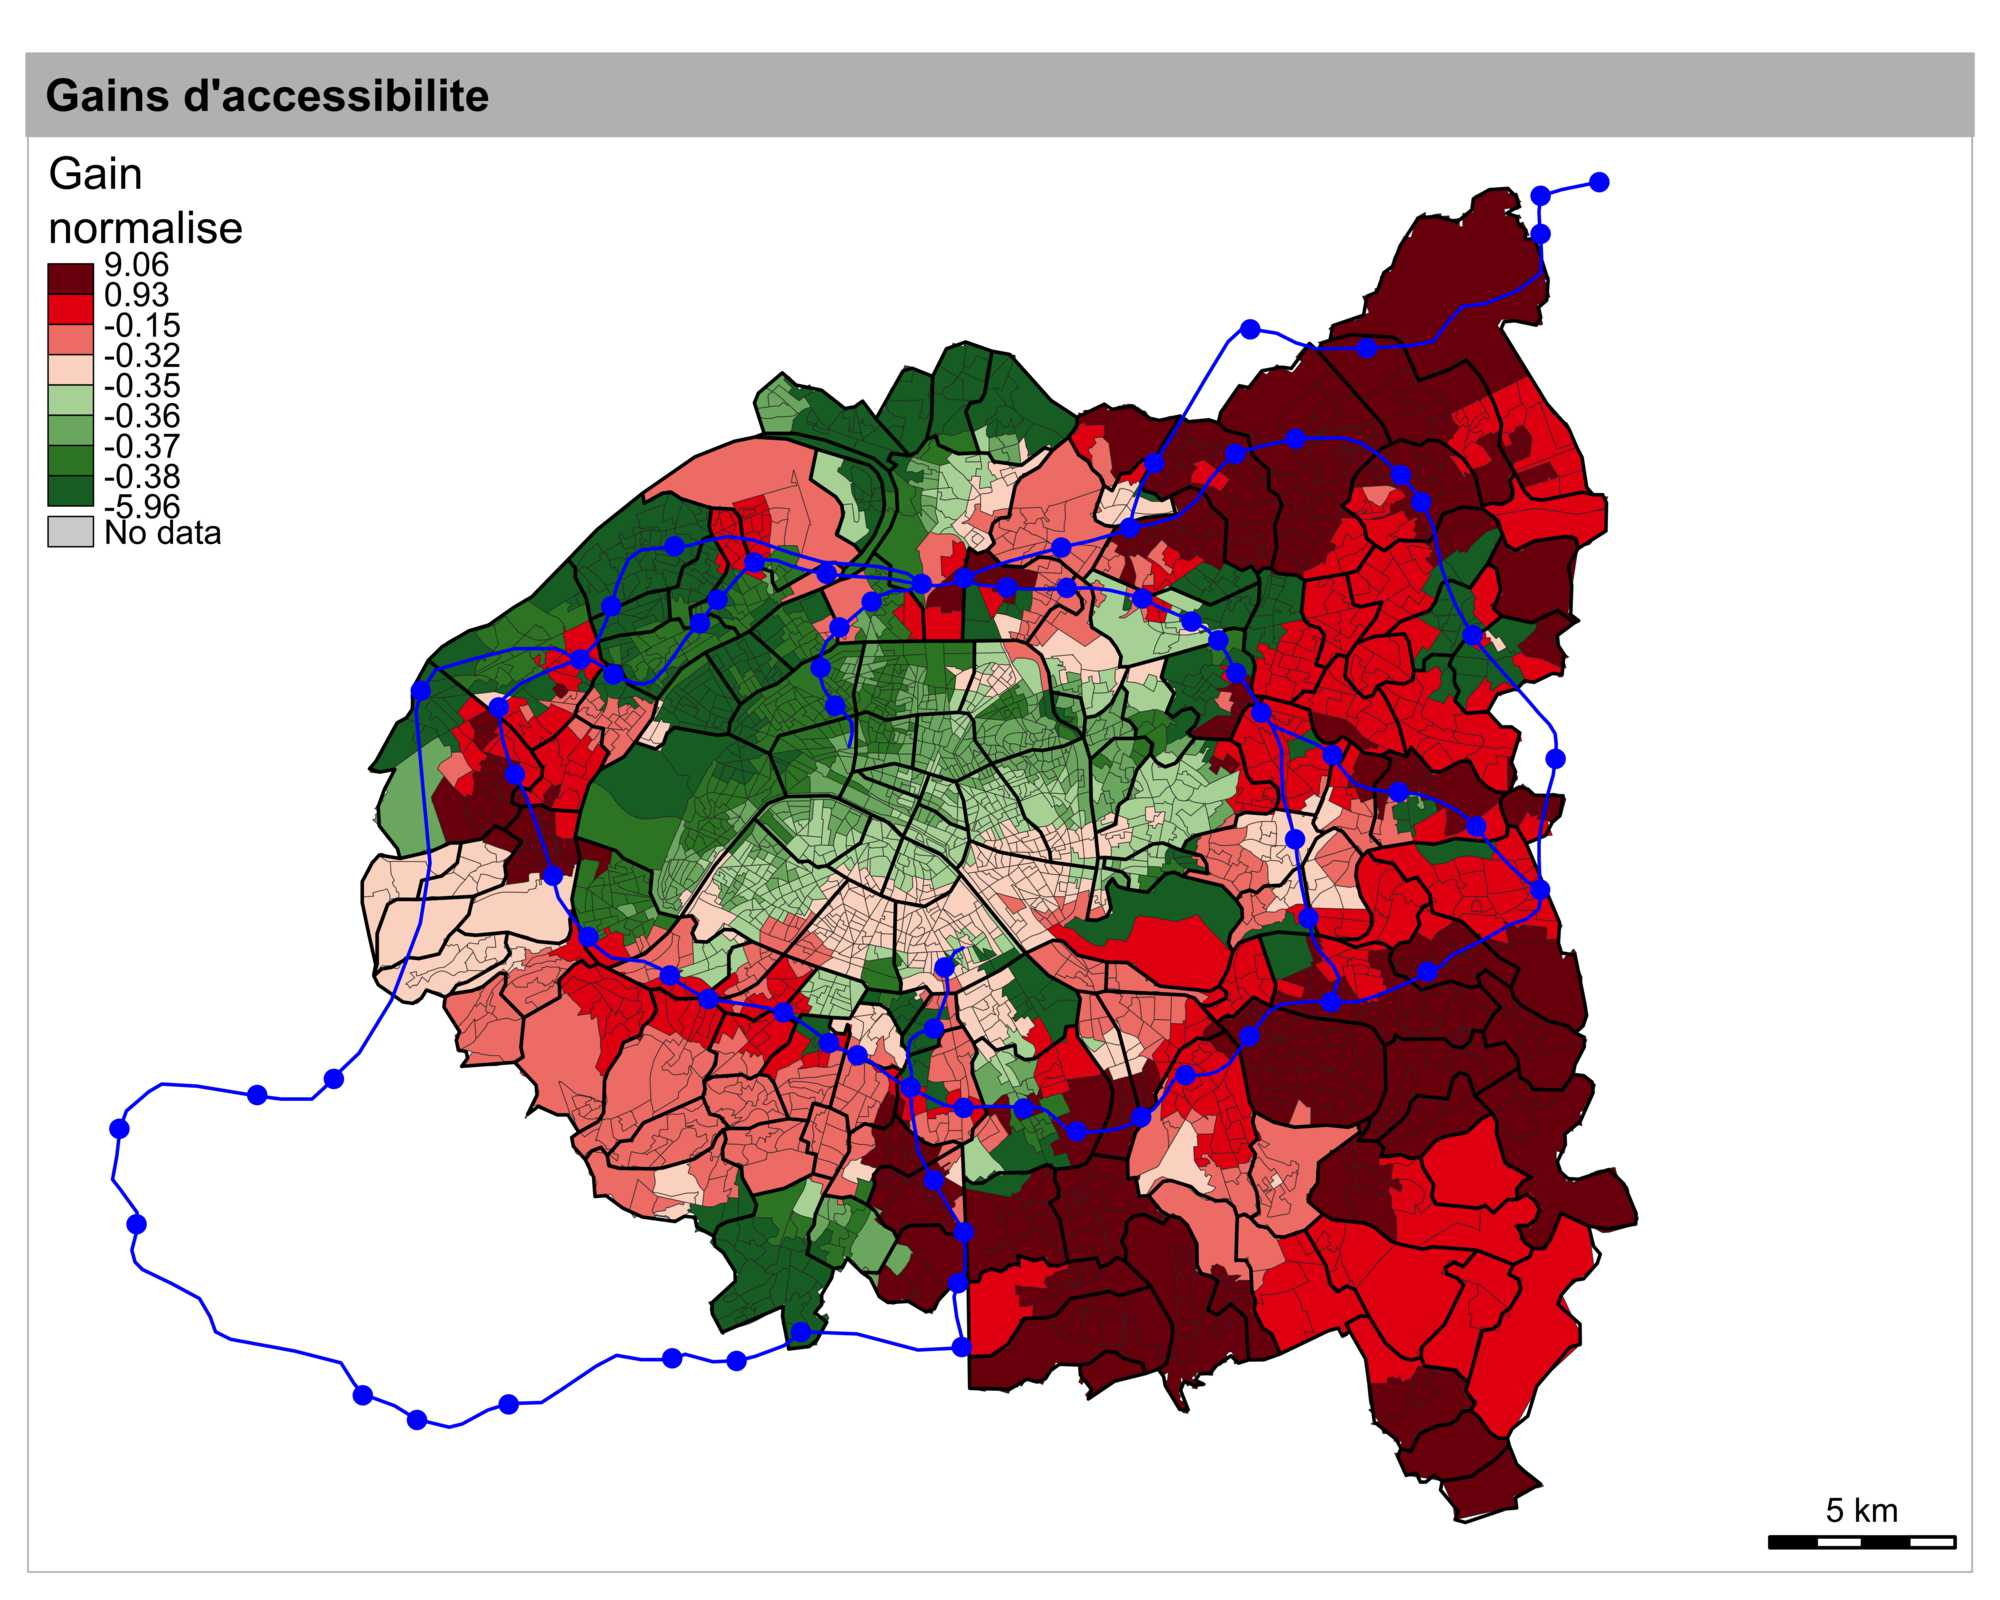
\includegraphics[width=\textwidth]{figures/4-grdparis.jpg}
\end{column}
\end{columns}

% LEGENDES

%\hspace{0.3cm}

}









%%%%%
%% Slide 8
%%%%%

\sframe{Modèles macroscopiques}{

}

%%%%%
%% Slide 9
%%%%%

\sframe{Modèles mesoscopiques}{

}



%%%%%
%% Slide 10
%%%%%

\sframe{Ouvertures}{

% Vers des théories intégratives des systèmes territoriaux

% donner des pistes
% theorique, epistemo quanti
% ici parler des developpements Lutecia : modeles.
% multi-modeling
%. -> bien parler de tous les domaines.
%. certains elements plus tangibles : va dans le sens de Morency : compris que quelque chose ici. : strqtgeie explorqtion ; redeveloppement langages scalable. : fait comprendre que chapitre creuser pas possible tel quel, passage a l'echelle necessaire, etc.
% 
% slide de fin : riche, permet ouverture.
%
% 


}



% PAS DE RESERVE SLIDES
% mais : obligation de moyens -> tableau, imager, graphes.




%%%%%%%%%%%%%%%%%%%%%
\begin{frame}[allowframebreaks]
\frametitle{References}
\bibliographystyle{apalike}
\bibliography{biblio}
\end{frame}
%%%%%%%%%%%%%%%%%%%%%%%%%%%%



%%%%%
%% Below : slides de la reunion equipe -> select some as reserve slides





%
%\sframe{Complex processes of Urban Morphogenesis}{
%
%\centering
%
%% center of Paris
%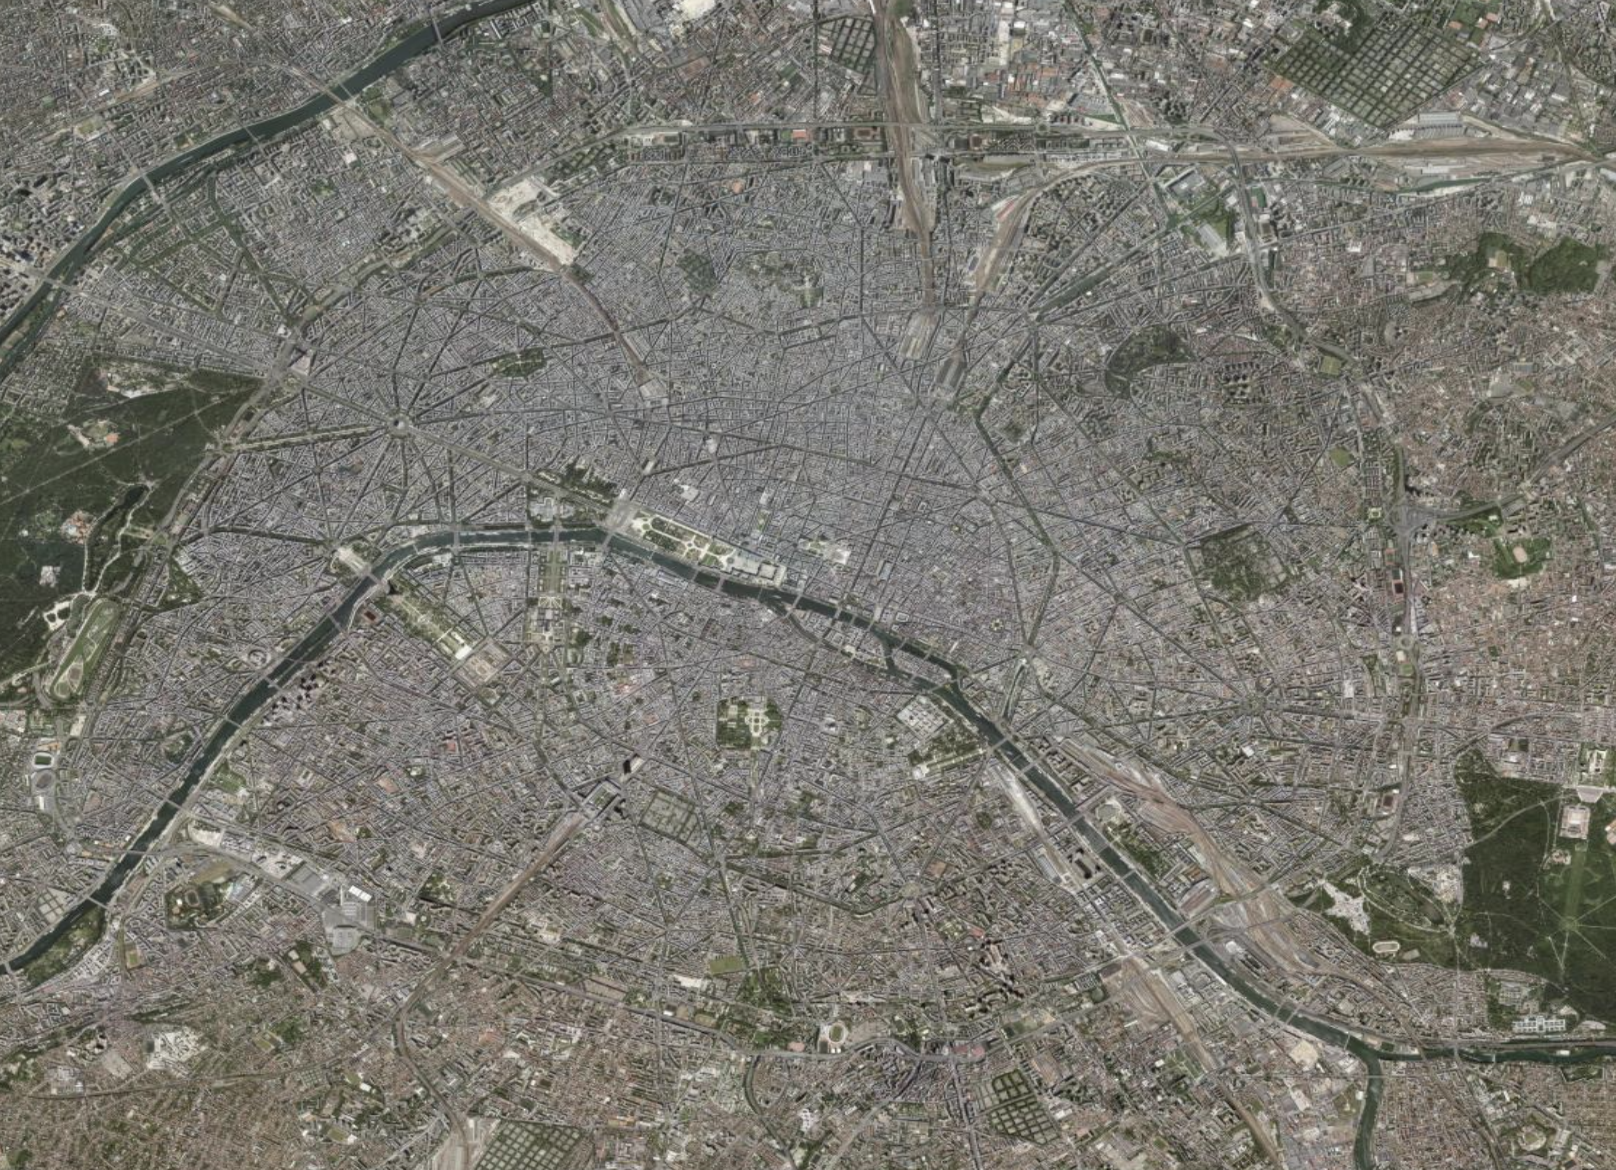
\includegraphics[width=0.9\textwidth]{figures/intro_paname}
%
%\footnotesize\textit{Source: Geoportail}
%}
%
%\sframe{Complex processes of Urban Morphogenesis}{
%
%\centering
%
%% large bp
%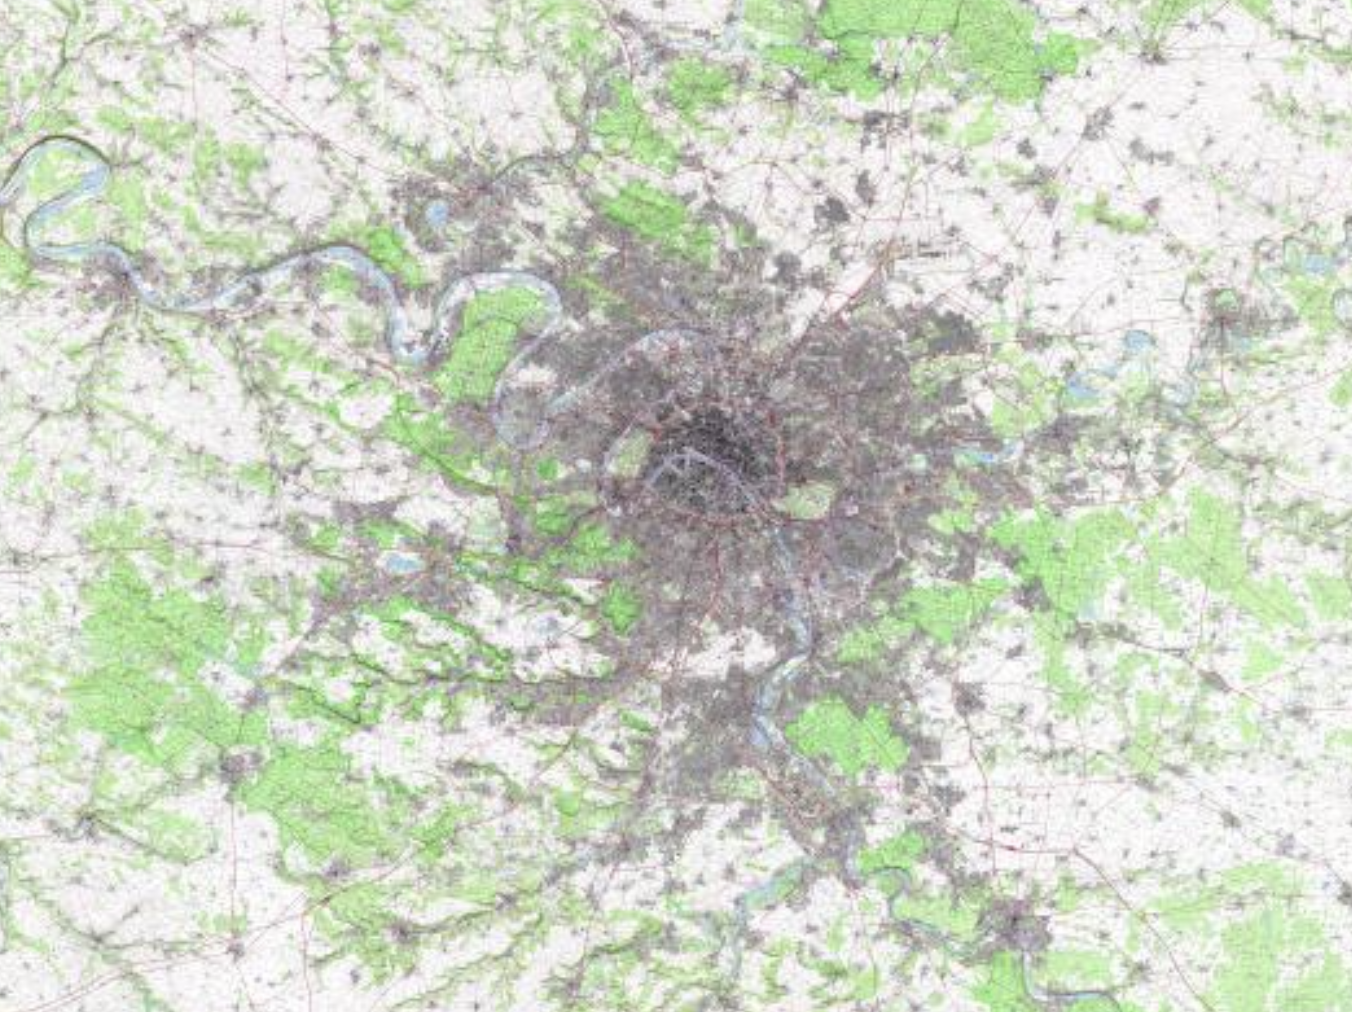
\includegraphics[width=0.9\textwidth]{figures/intro_bp}
%
%\footnotesize\textit{Source: Geoportail}
%}
%
%
%
%\sframe{What is Morphogenesis ?}{
%
%\textbf{Morphogenesis} (\textit{Oxford dictionary}) 
%\begin{enumerate}
%\item \textit{Biology} : The origin and development of morphological characteristics
%\item \textit{Geology} : The formation of landforms or other structures.
%\end{enumerate}
%
%\bigskip
%
%\textbf{History of the notion}
%
%$\rightarrow$ Started significantly with embryology around 1930~\cite{abercrombie1977concepts} 
%
%$\rightarrow$ Turing's 1952 paper~\cite{turing1952chemical}, linked to the development of Cybernetics
%
%$\rightarrow$ first use in 1871, large peak in usage between 1907-1909, increase until 1990, decrease until today. \textit{Scientific fashion ?}
%
%
%}
%
%
%
%
%
%\sframe{What is Morphogenesis ? Examples}{
%
%% illustrations : ants, geomorphology, neurons, self-assembly ; ARBOTRON ; paper nature aile avion
%% all from netlogo library ? would be nice illustration of generative nature
%
%
%% remark : do not put classical biological example to show how it has percolated to other fields
%
%\vspace{-0.3cm}
%
%\includegraphics[width=\textwidth,height=0.82\textheight]{figures/intro_examples}
%
%\justify
%
%\vspace{-0.5cm}
%
%\footnotesize\textit{Sources (in order by column). Ants, Erosion, Game of Life: NetLogo Library ; Arbotron \cite{jun2005formation}; Industrial design \cite{Aage:2017aa}; Swarm chemistry \cite{sayama2007decentralized}}
%% sources : ants netlogo ; erosion netlogo ; arbotron 
%%  inge : 
%
%}
%
%
%
%\sframe{Defining Morphogenesis}{
%
%% precise notions and defs
%
%\justify
%
%\textit{Construction of an interdisciplinary definition in~\cite{antelope2016interdisciplinary}}
%
%\bigskip
%
%
%
%
%\textbf{Meta-epistemological framework of imbricated notions:}
%
%Self-organization $\supsetneq$ Morphogenesis $\supsetneq$ Autopoiesis $\supsetneq$ Life
%
%
%\bigskip
%
%\textbf{Properties:}
%
%\begin{itemize}
%\item Architecture links form and function
%\item Emergence strength~\cite{bedau2002downward} increases with notion depth, as bifurcations~\cite{thom1974stabilite}
%\end{itemize}
%
%\bigskip
%
%\textbf{Definition of Morphogenesis :} \textit{Emergence of the form and the function in a strongly coupled manner, producing an emergent architecture \cite{doursat2012morphogenetic}}
%
%
%
%}
%
%
%
%\sframe{Which models for Urban Morphogenesis ?}{
%
%% why modeling, exemple of rbd
%% -> champ ; difficultés ("verrous". rq : j'aime pas la metaphore du verrou, trop cadrant et suppose que deja construit et qu'il suffit d'ouvrir. demarche epistemo de co-evol des connaissances, ni inductif ni deductif. il faut contruire. horizons d'exploration plus appropriés. rejoint l'idee de faire rentrer dans "cadre analytique" : cases prédéfinies, alors qu'il s'agit au contraire de définir ces cases. -> relire hdr arnaud
%
%\justify
%
%\begin{columns}
%\column{0.4\textwidth}
%\centering
%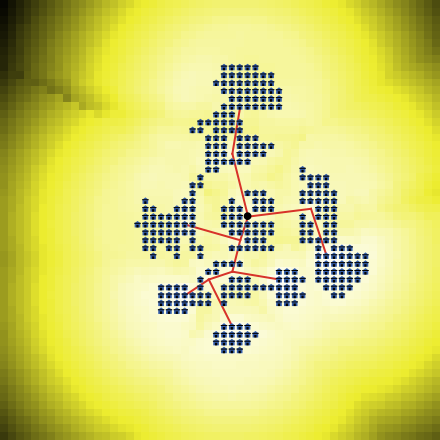
\includegraphics[width=\textwidth]{figures/intro_RBD_lattice}\\
%\footnotesize\textit{Example: a basic hybrid model based on elementary processes for density and network \cite{raimbault2014hybrid}}
%\column{0.57\textwidth}
%\justify
%
%%\vspace{-1cm}
%
%$\rightarrow$\textit{At the crossroad between Urban Simulation and Artificial Life, few models try to integrate and explain the link between Urban Form and Function}
%
%\medskip
%
%$\rightarrow$\textit{Importance of parcimonious, stylized models: modeling as a tool to understand processes}
%
%\end{columns}
%
%\bigskip
%
%\textbf{Research Objective : } Explore simple models to capture morphogenesis based on abstract representation of urban processes; test their ability to reproduce existing urban systems.
%
%
%
%}
%
%
%\sframe{A simple Reaction-diffusion model}{
%
%% comment Arnaud : reaction-diffusion ?
%
%% model rationale and processes
%
%
%\justify
%
%$\rightarrow$ Crucial role of the interplay between concentration forces and dispersion forces~\cite{fujita1996economics} in keeping Urban Systems at the border of chaos
%
%\bigskip
%
%$\rightarrow$ Potentiality of aggregation mechanisms (such as Simon model) to produce power laws \cite{2016arXiv160806313S}
%
%\bigskip
%
%$\rightarrow$ Link with Reaction-diffusion approaches in Morphogenesis~\cite{turing1952chemical}
%
%\bigskip
%
%$\rightarrow$ Extension of a DLA-type model introduced by \cite{batty1991generating}, with simple abstract processes of population aggregation and diffusion
%
%}
%
%\sframe{Model Formalization}{
%
%% model formalization and indicators
%
%$\rightarrow$ Grid world with cell populations $(P_i(t))_{1\leq i\leq N^2}$.
%
%\bigskip
%
%$\rightarrow$ At each time step:
%
%% comment Arnaud : si tu beamais pas tu pourrais introduire une video du modèle ;-)
%
%\begin{enumerate}
%\item Population growth with exogenous rate $N_G$, attributed independently to a cell following a preferential attachment of strength $\alpha$
%%\begin{equation}
%%\Pb{P_i(t+1)=P_i(t)+1|P(t+1)=P(t)+1}=\frac{(P_i(t)/P(t))^{\alpha}}{\sum(P_i(t)/P(t))^{\alpha}}
%%\end{equation}
%%The attribution being uniformly drawn if all population are equal to 0.
%\item Population is diffused $n_d$ times with strength $\beta$
%\end{enumerate}
%
%\bigskip
%
%$\rightarrow$ Stopping criterion: fixed maximal population $P_m$.
%
%%To avoid bord effects such as reflecting diffusion waves, border cells diffuse their due proportion outside of the world, implying that the total population at time $t$ is strictly smaller than $N_G\cdot t$.
%
%\bigskip
%
%$\rightarrow$ Output measured by morphological indicators: Moran index, average distance, rank-size hierarchy, entropy.
%
%
%}
%
%
%\sframe{Generating Population Distributions}{
%
%
%% examples : fig 2 of paper
%
%\centering
%
%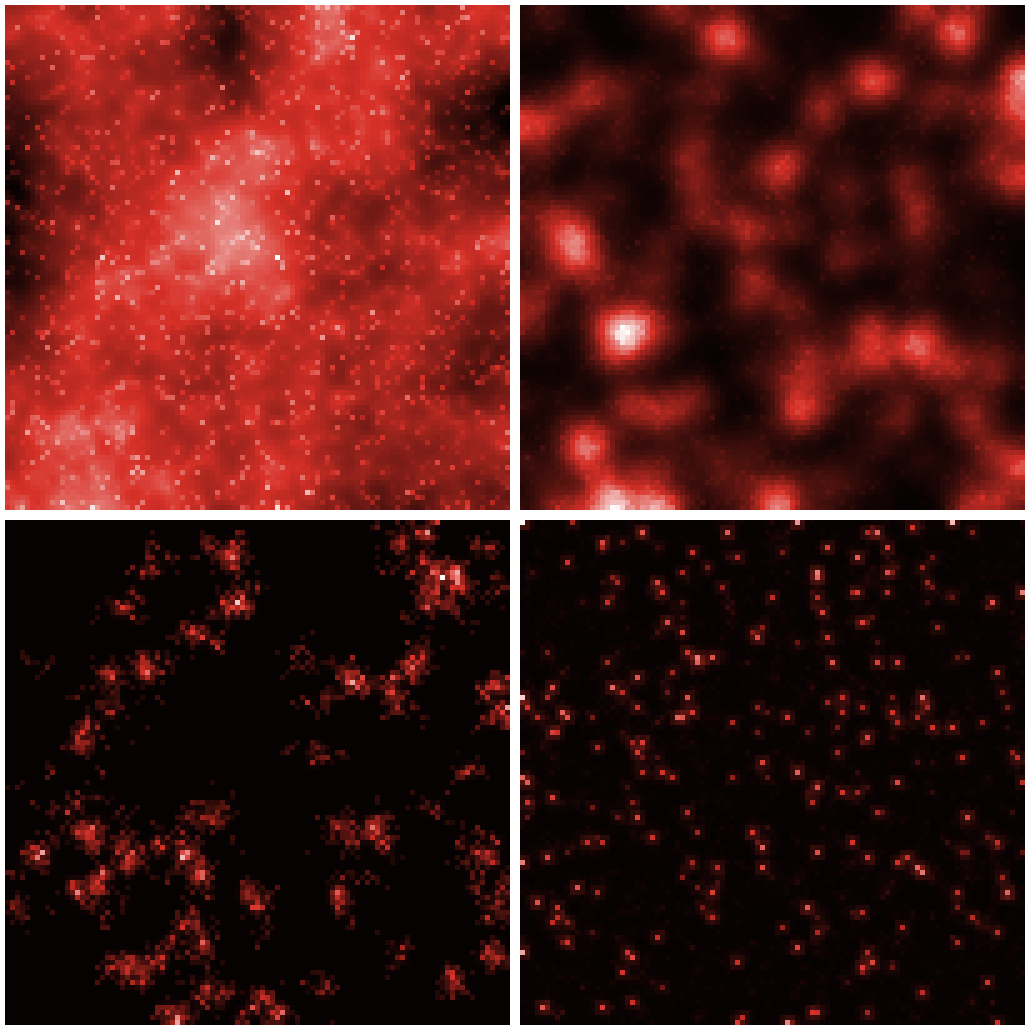
\includegraphics[height=0.8\textheight]{figures/density_Fig2}
%
%\footnotesize\textit{Examples of generated territorial shapes}
%
%}
%
%
%\sframe{Model behavior}{
%
%% comment Arnaud : Les graphiques correspondent aux 4 exemples précédents ? Si oui les rappeler en petite vignette. -> NON
%
%\centering
%
%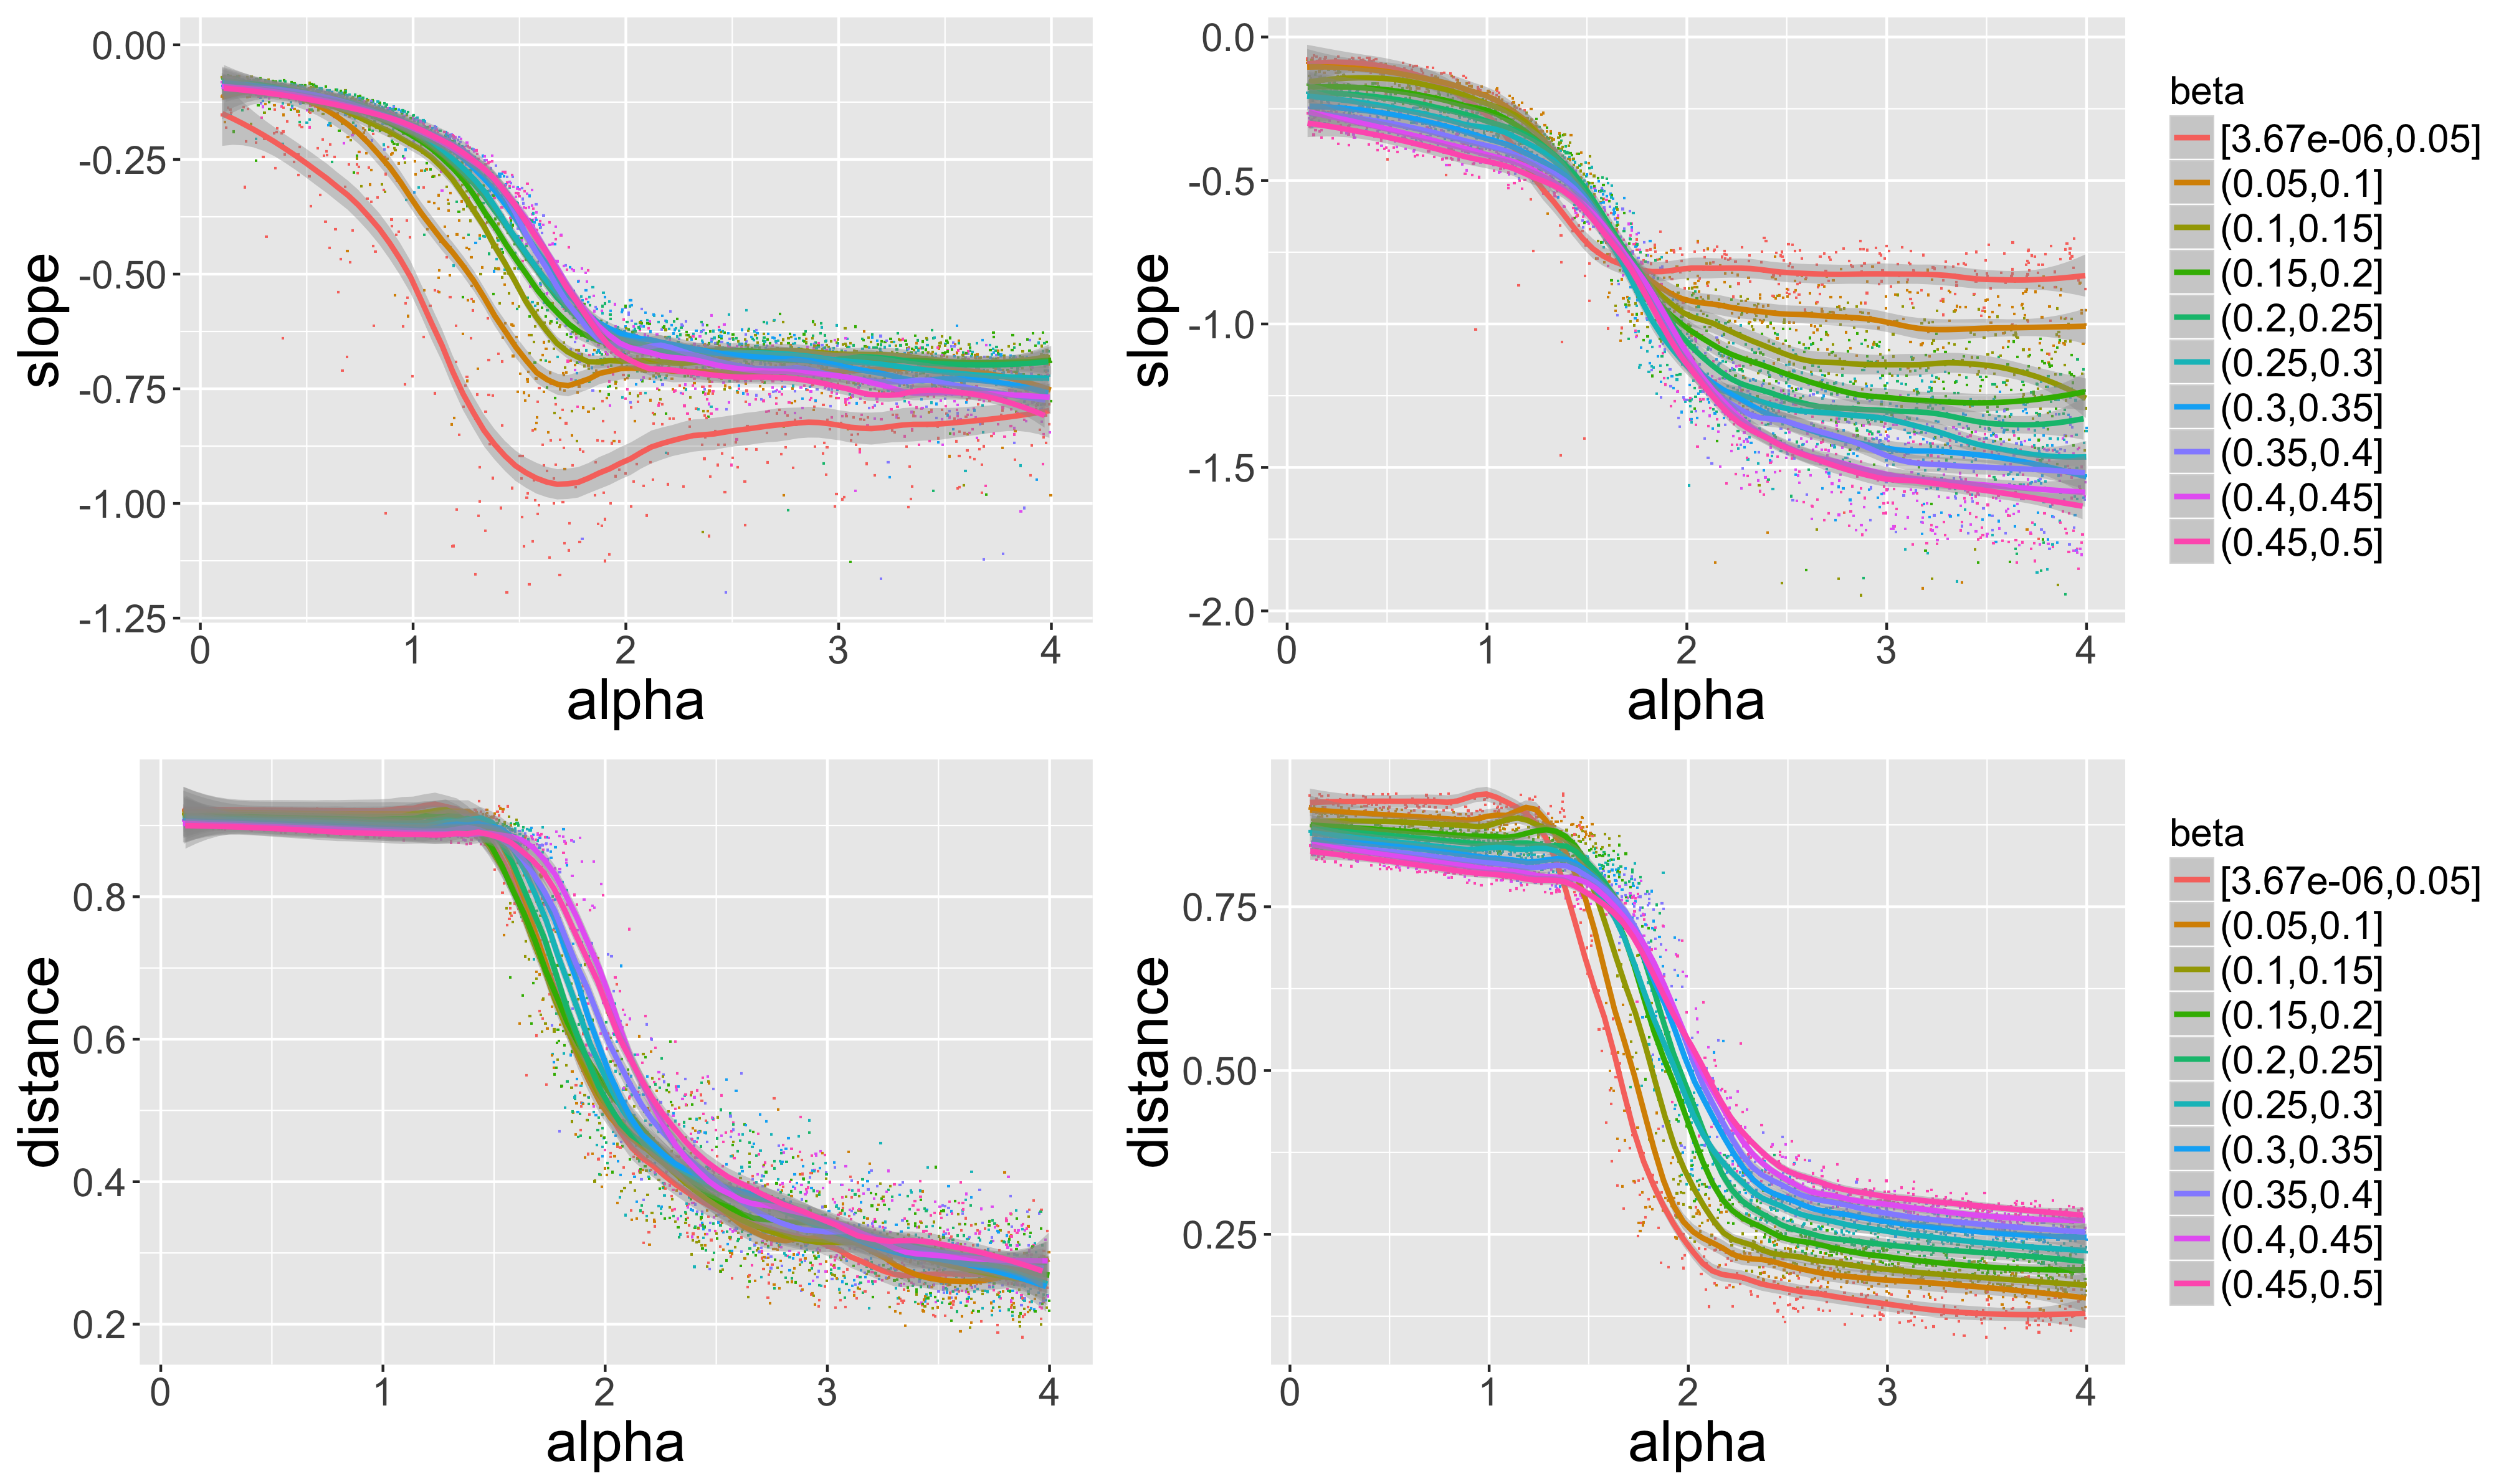
\includegraphics[width=0.9\textwidth]{figures/density_Fig3}
%
%\footnotesize\textit{Phase transitions of indicators unveiled by exploration of the parameter space (80000 parameter points, 10 repetitions each)}
%
%% comment Arnaud : Préciser (dimensionner)
%
%}
%
%
%
%
%\sframe{Path-dependence and frozen accidents}{
%
%\centering
%
%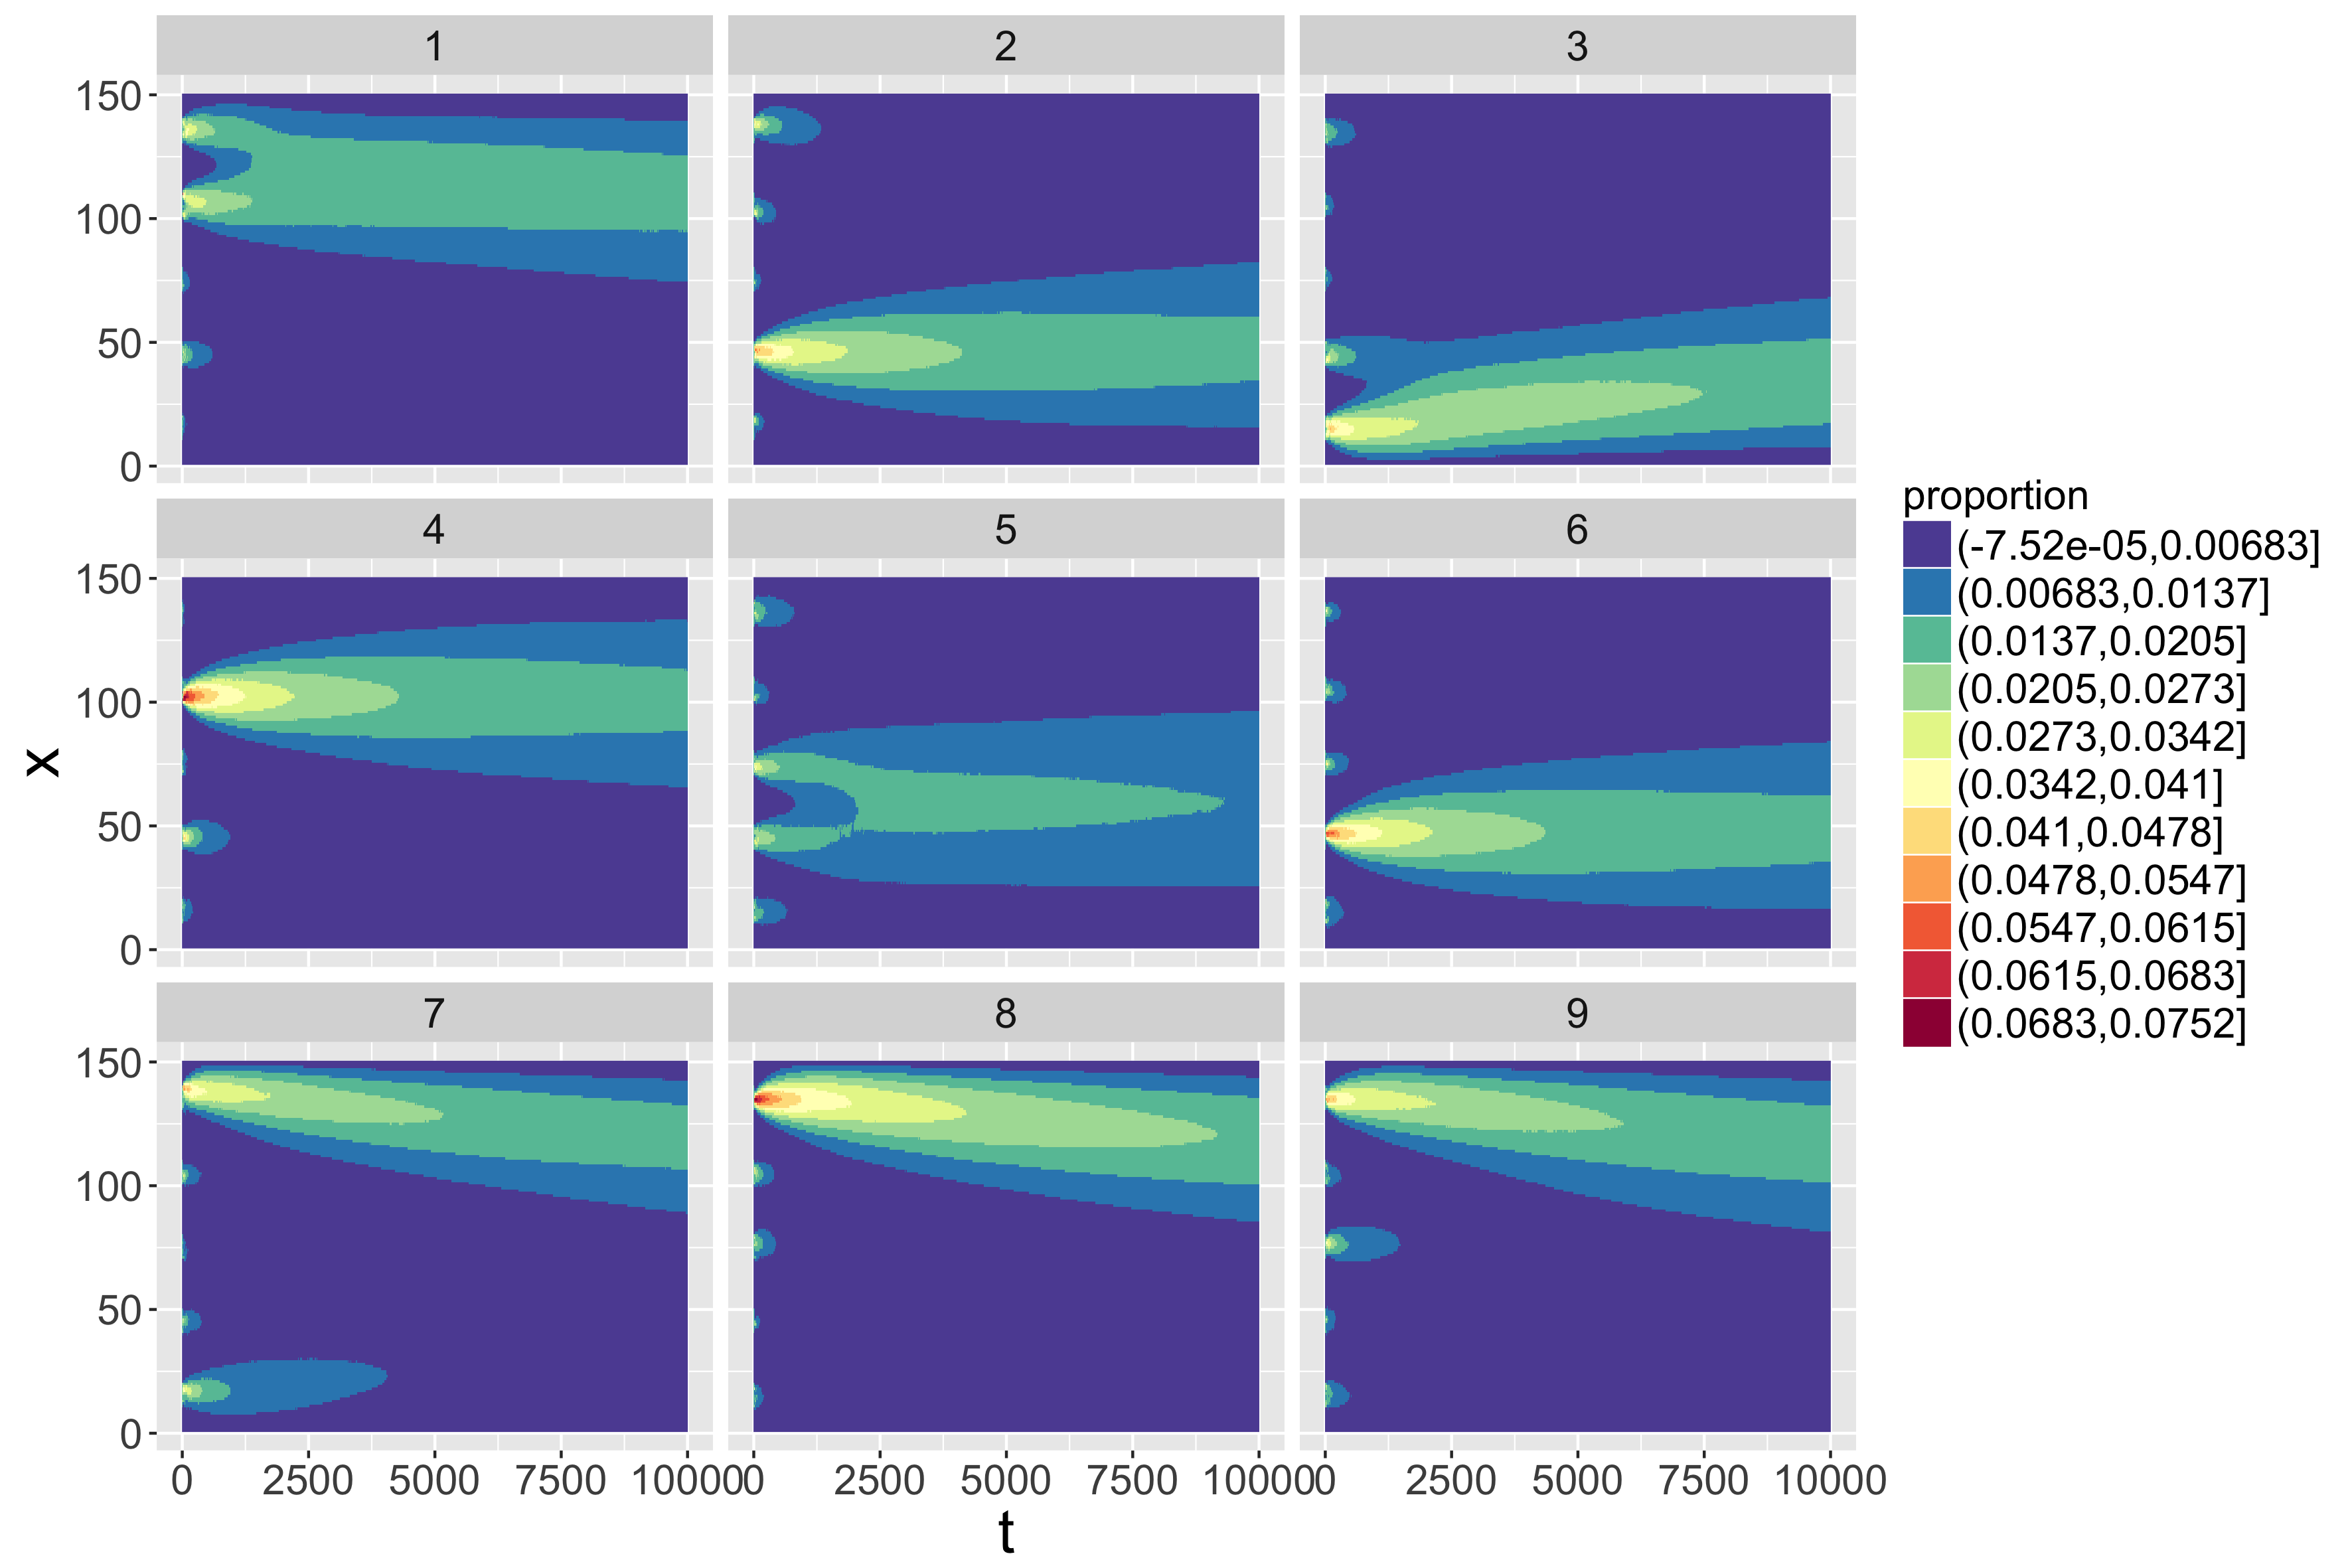
\includegraphics[width=0.8\textwidth]{figures/density_Fig4}
%
%\footnotesize\textit{Illustration of path-dependence in a simplified one-dimensional version of the model: cell trajectories in time for 9 independent repetitions from the same initial configuration.}
%
%
%}
%
%
%\sframe{Empirical Data for Calibration}{
%
%% comments Arnaud : Quel lien avec les slides avant et après ? "Real" : le terme me paraît discutable : données empiriques plutôt ?
%%  Décrire les données car ici tu passes directement aux indicateurs
%
%\begin{columns}
%\column{0.6\textwidth}
%\centering
%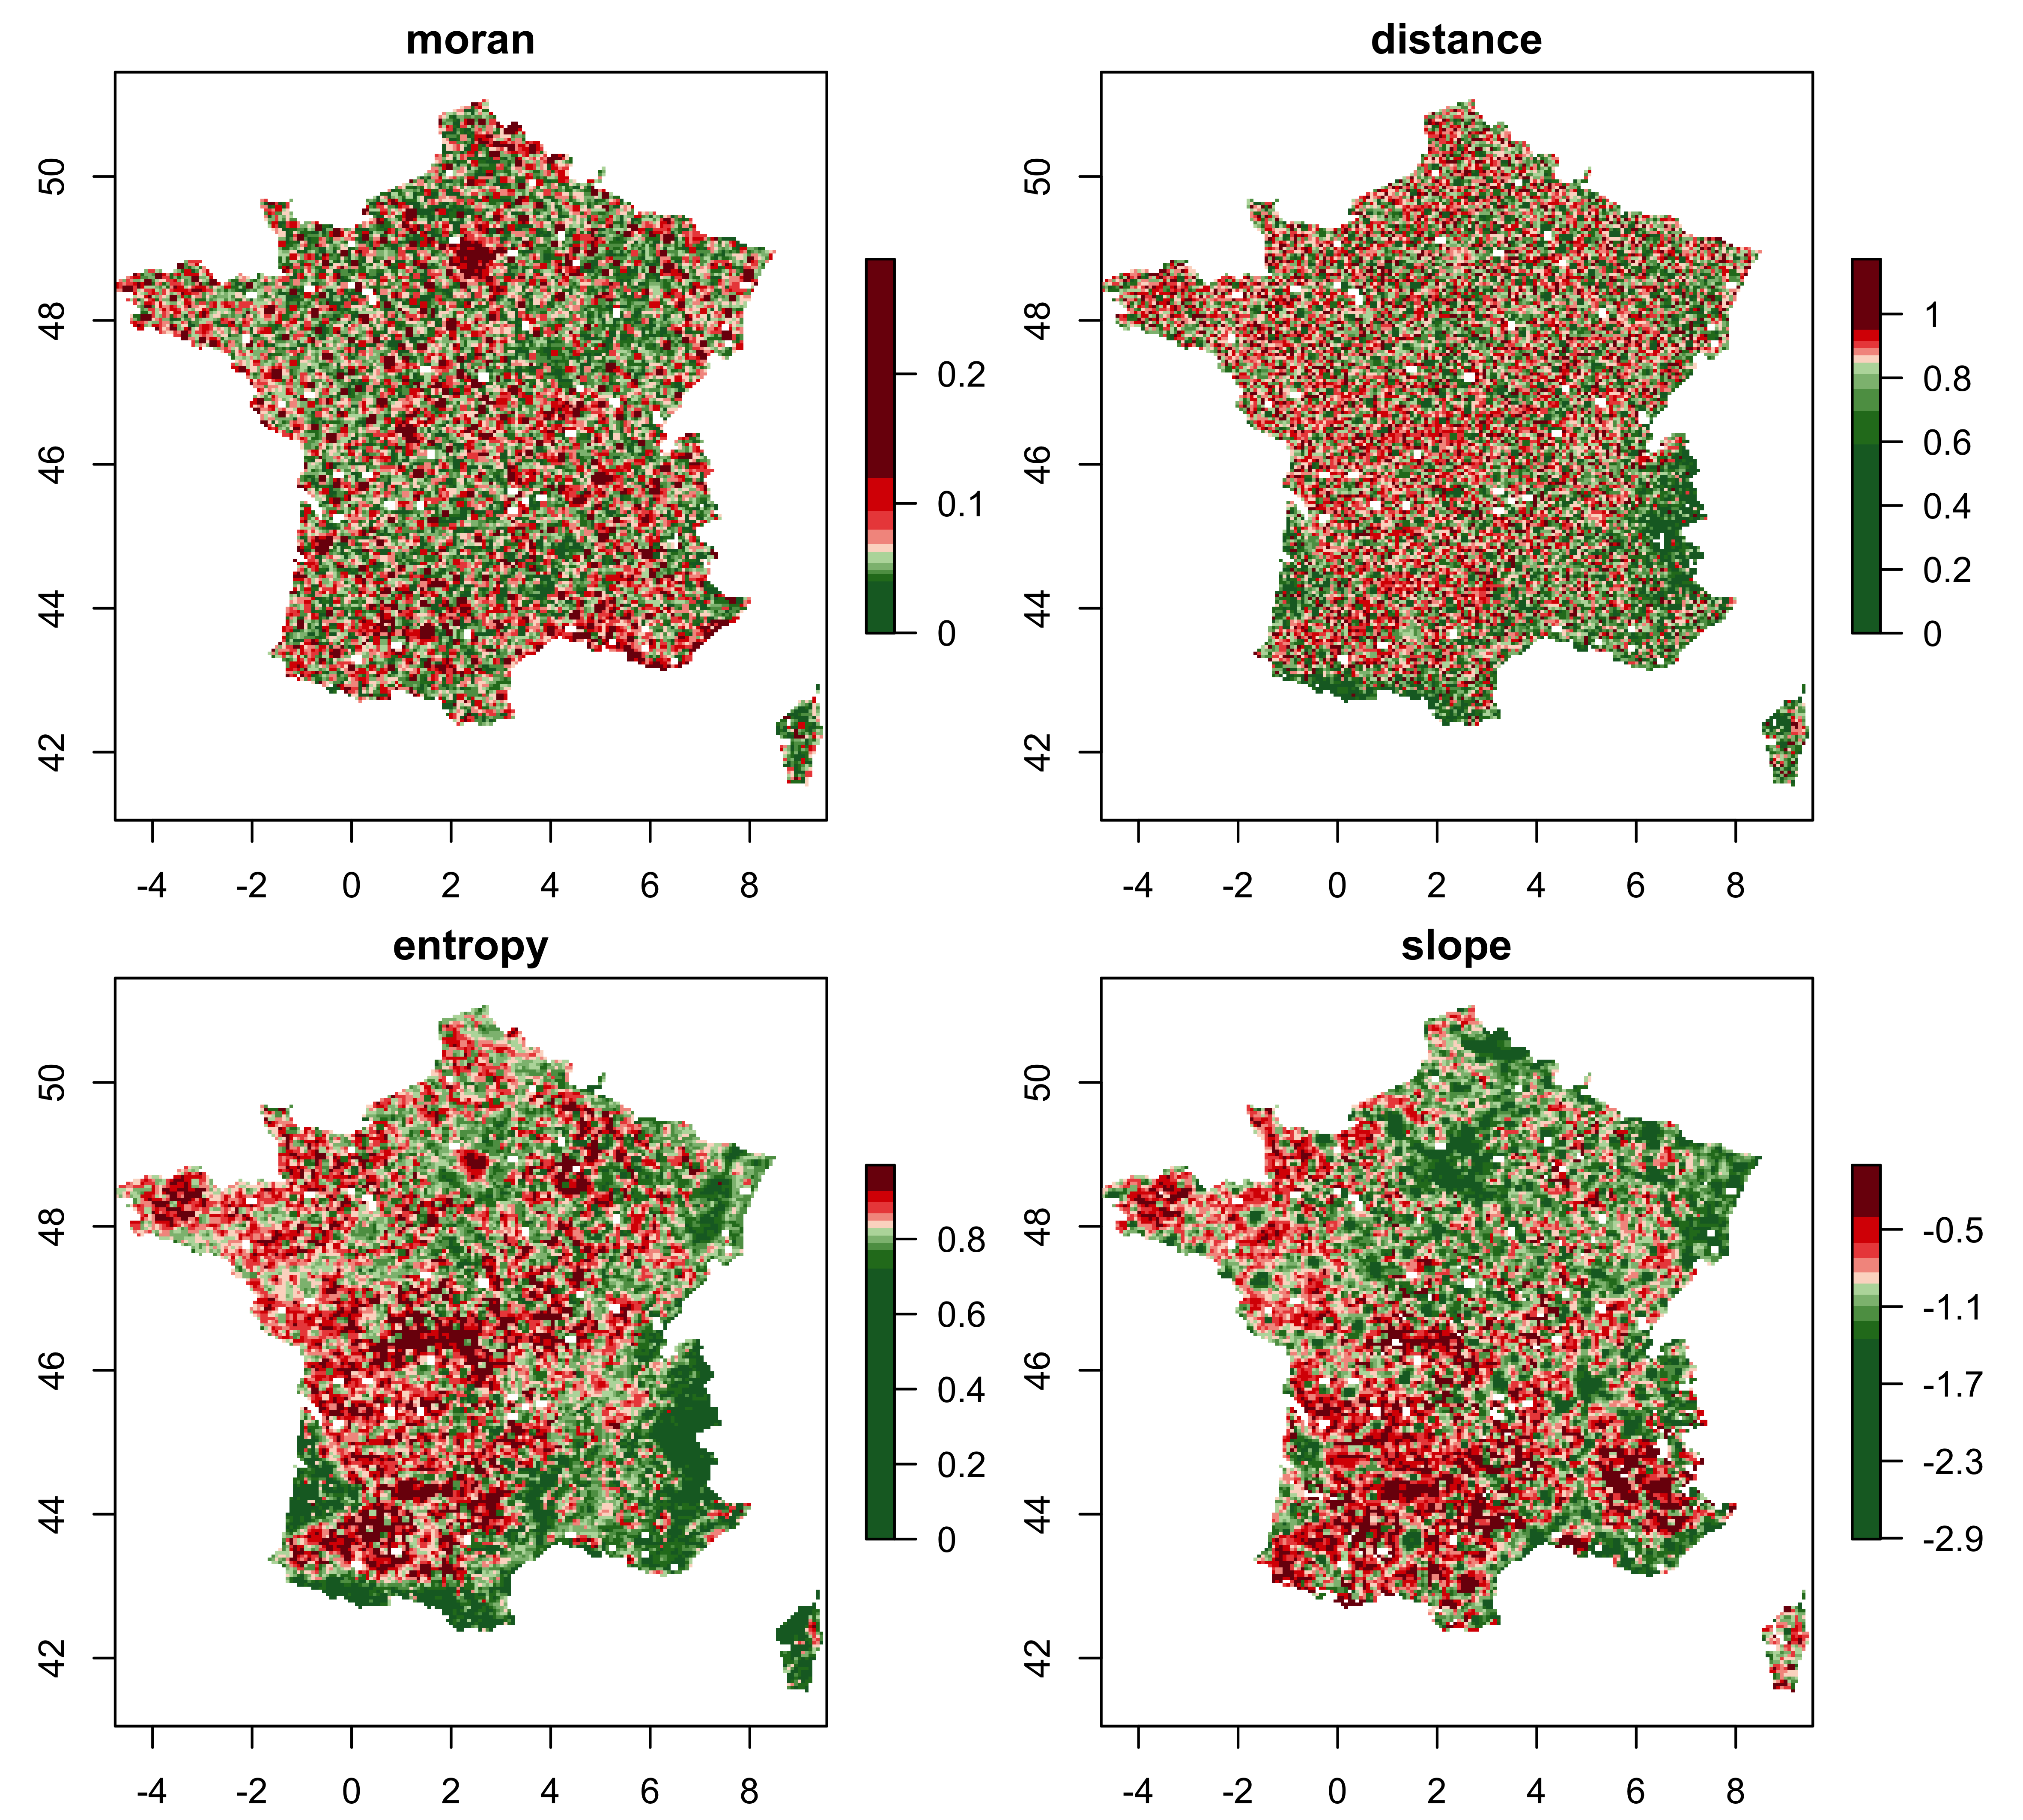
\includegraphics[width=\textwidth]{figures/density_indics_morpho_discrquantiles}
%\column{0.3\textwidth}
%\centering
%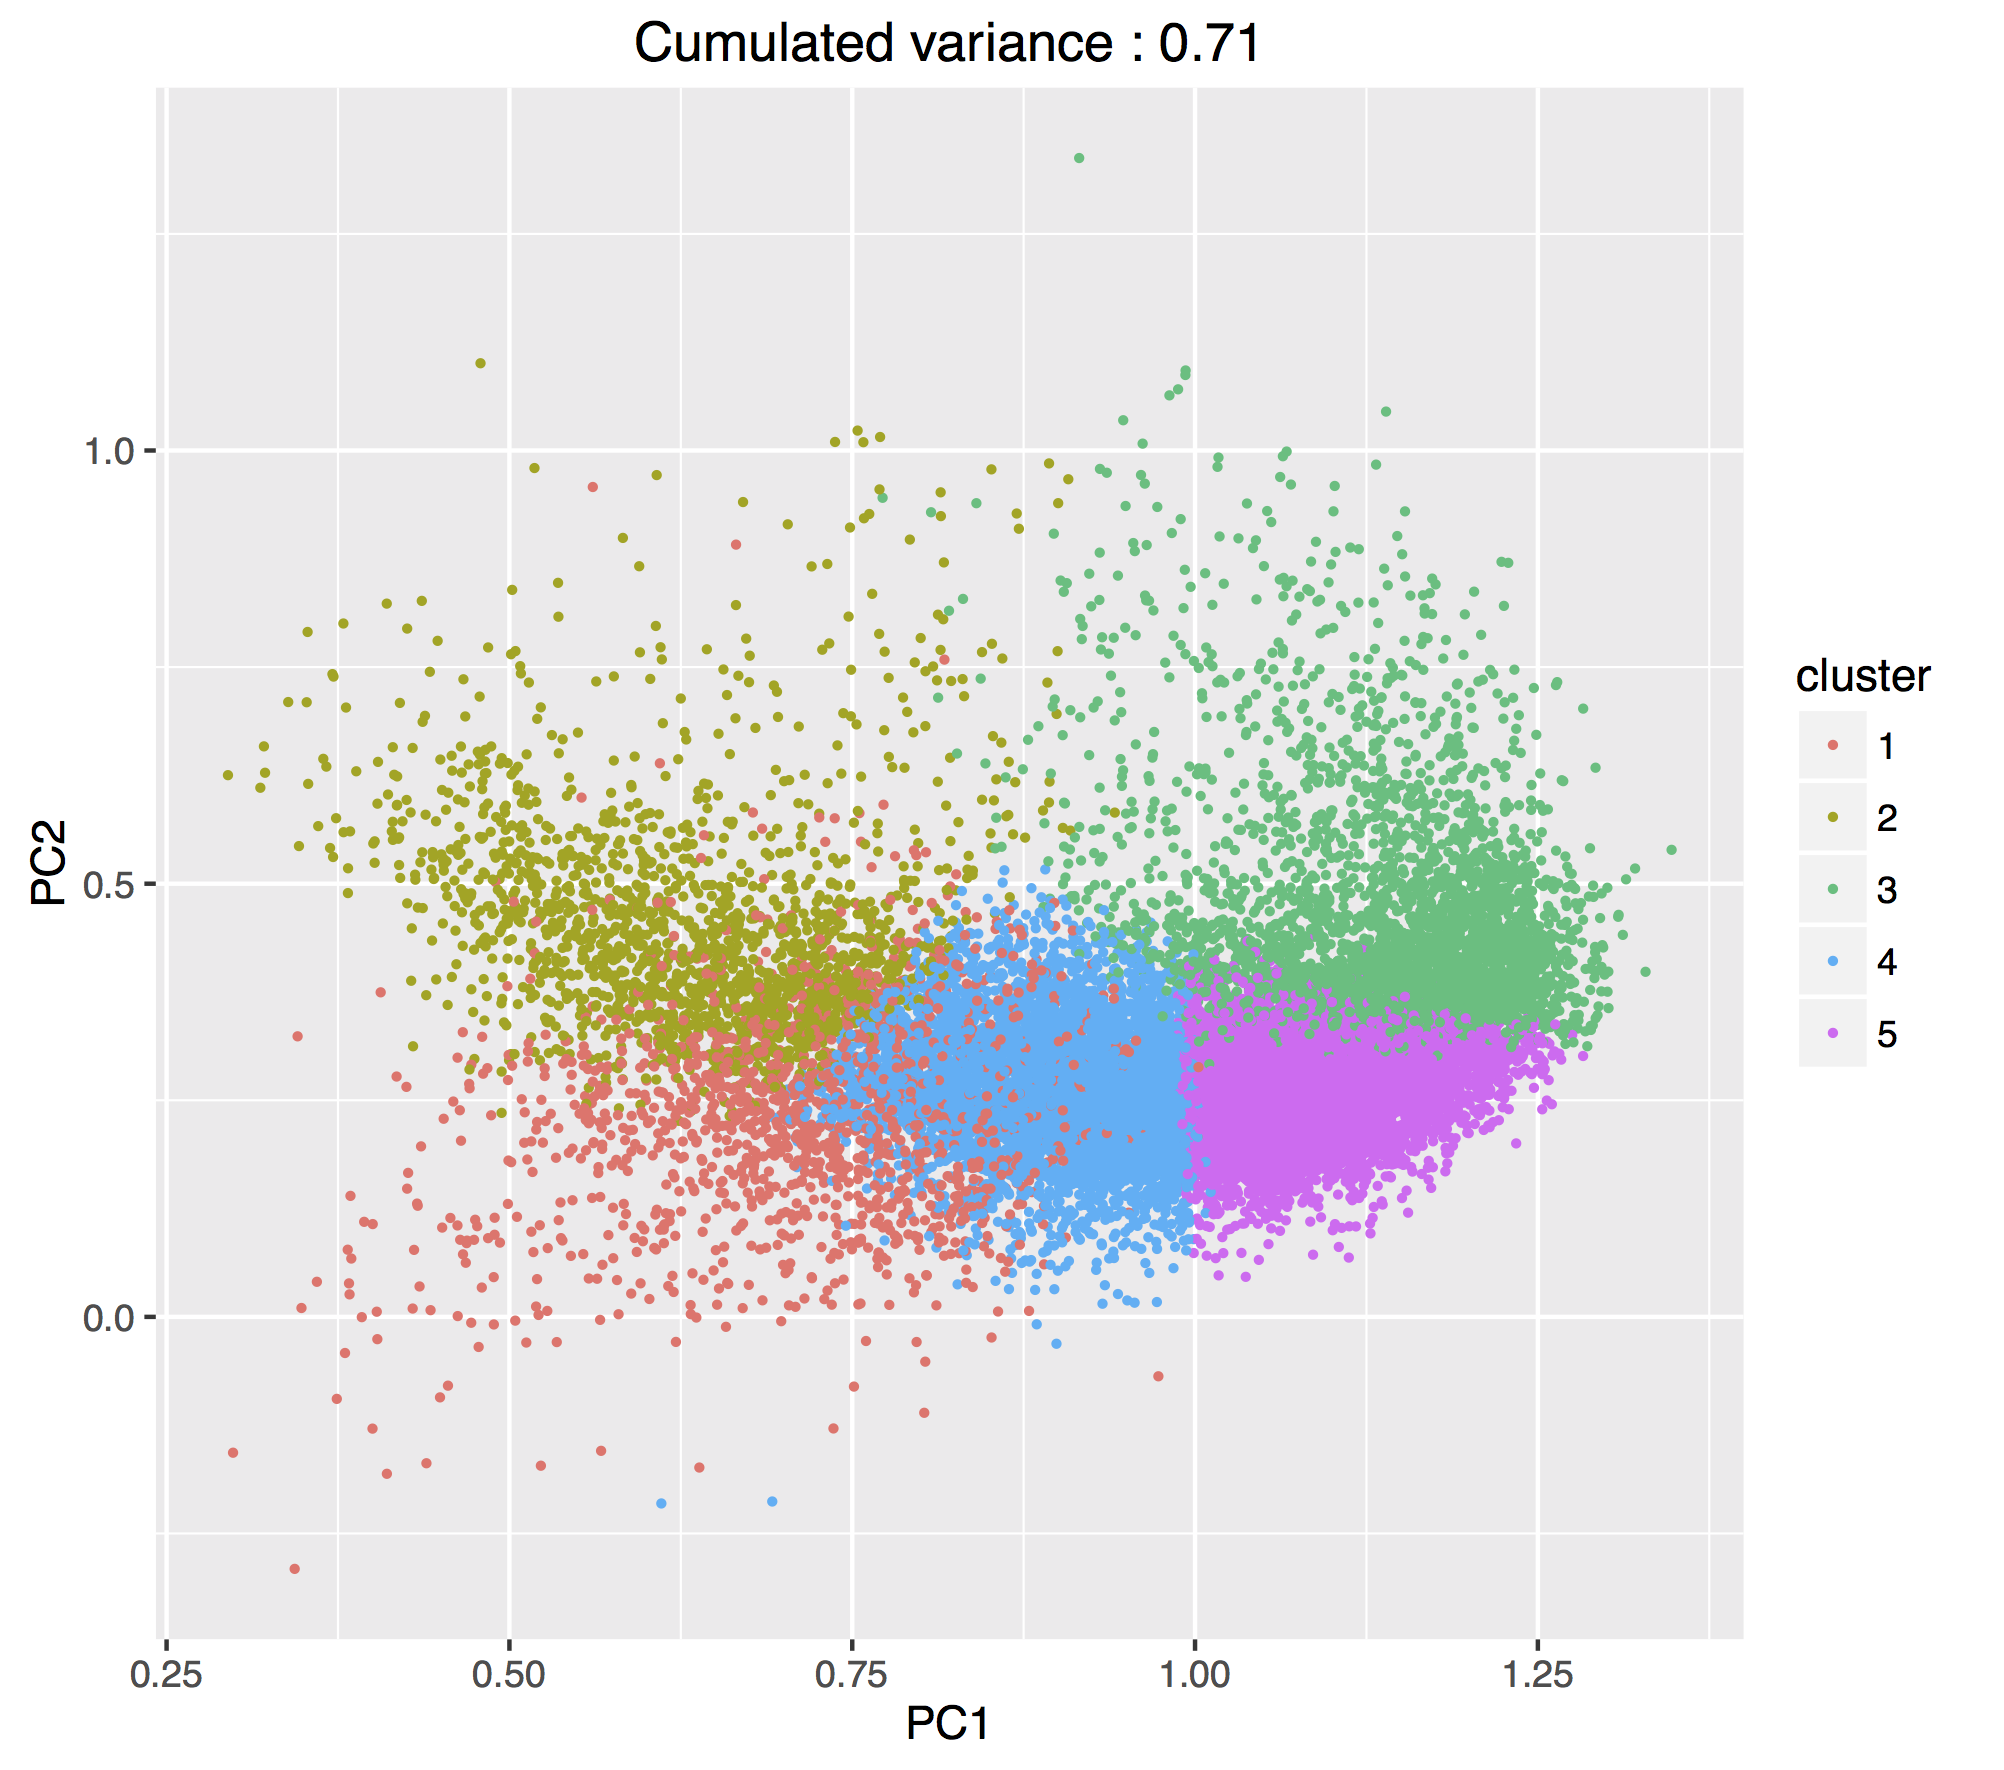
\includegraphics[width=\textwidth]{figures/density_cluster_pca_k5_morpho}\\
%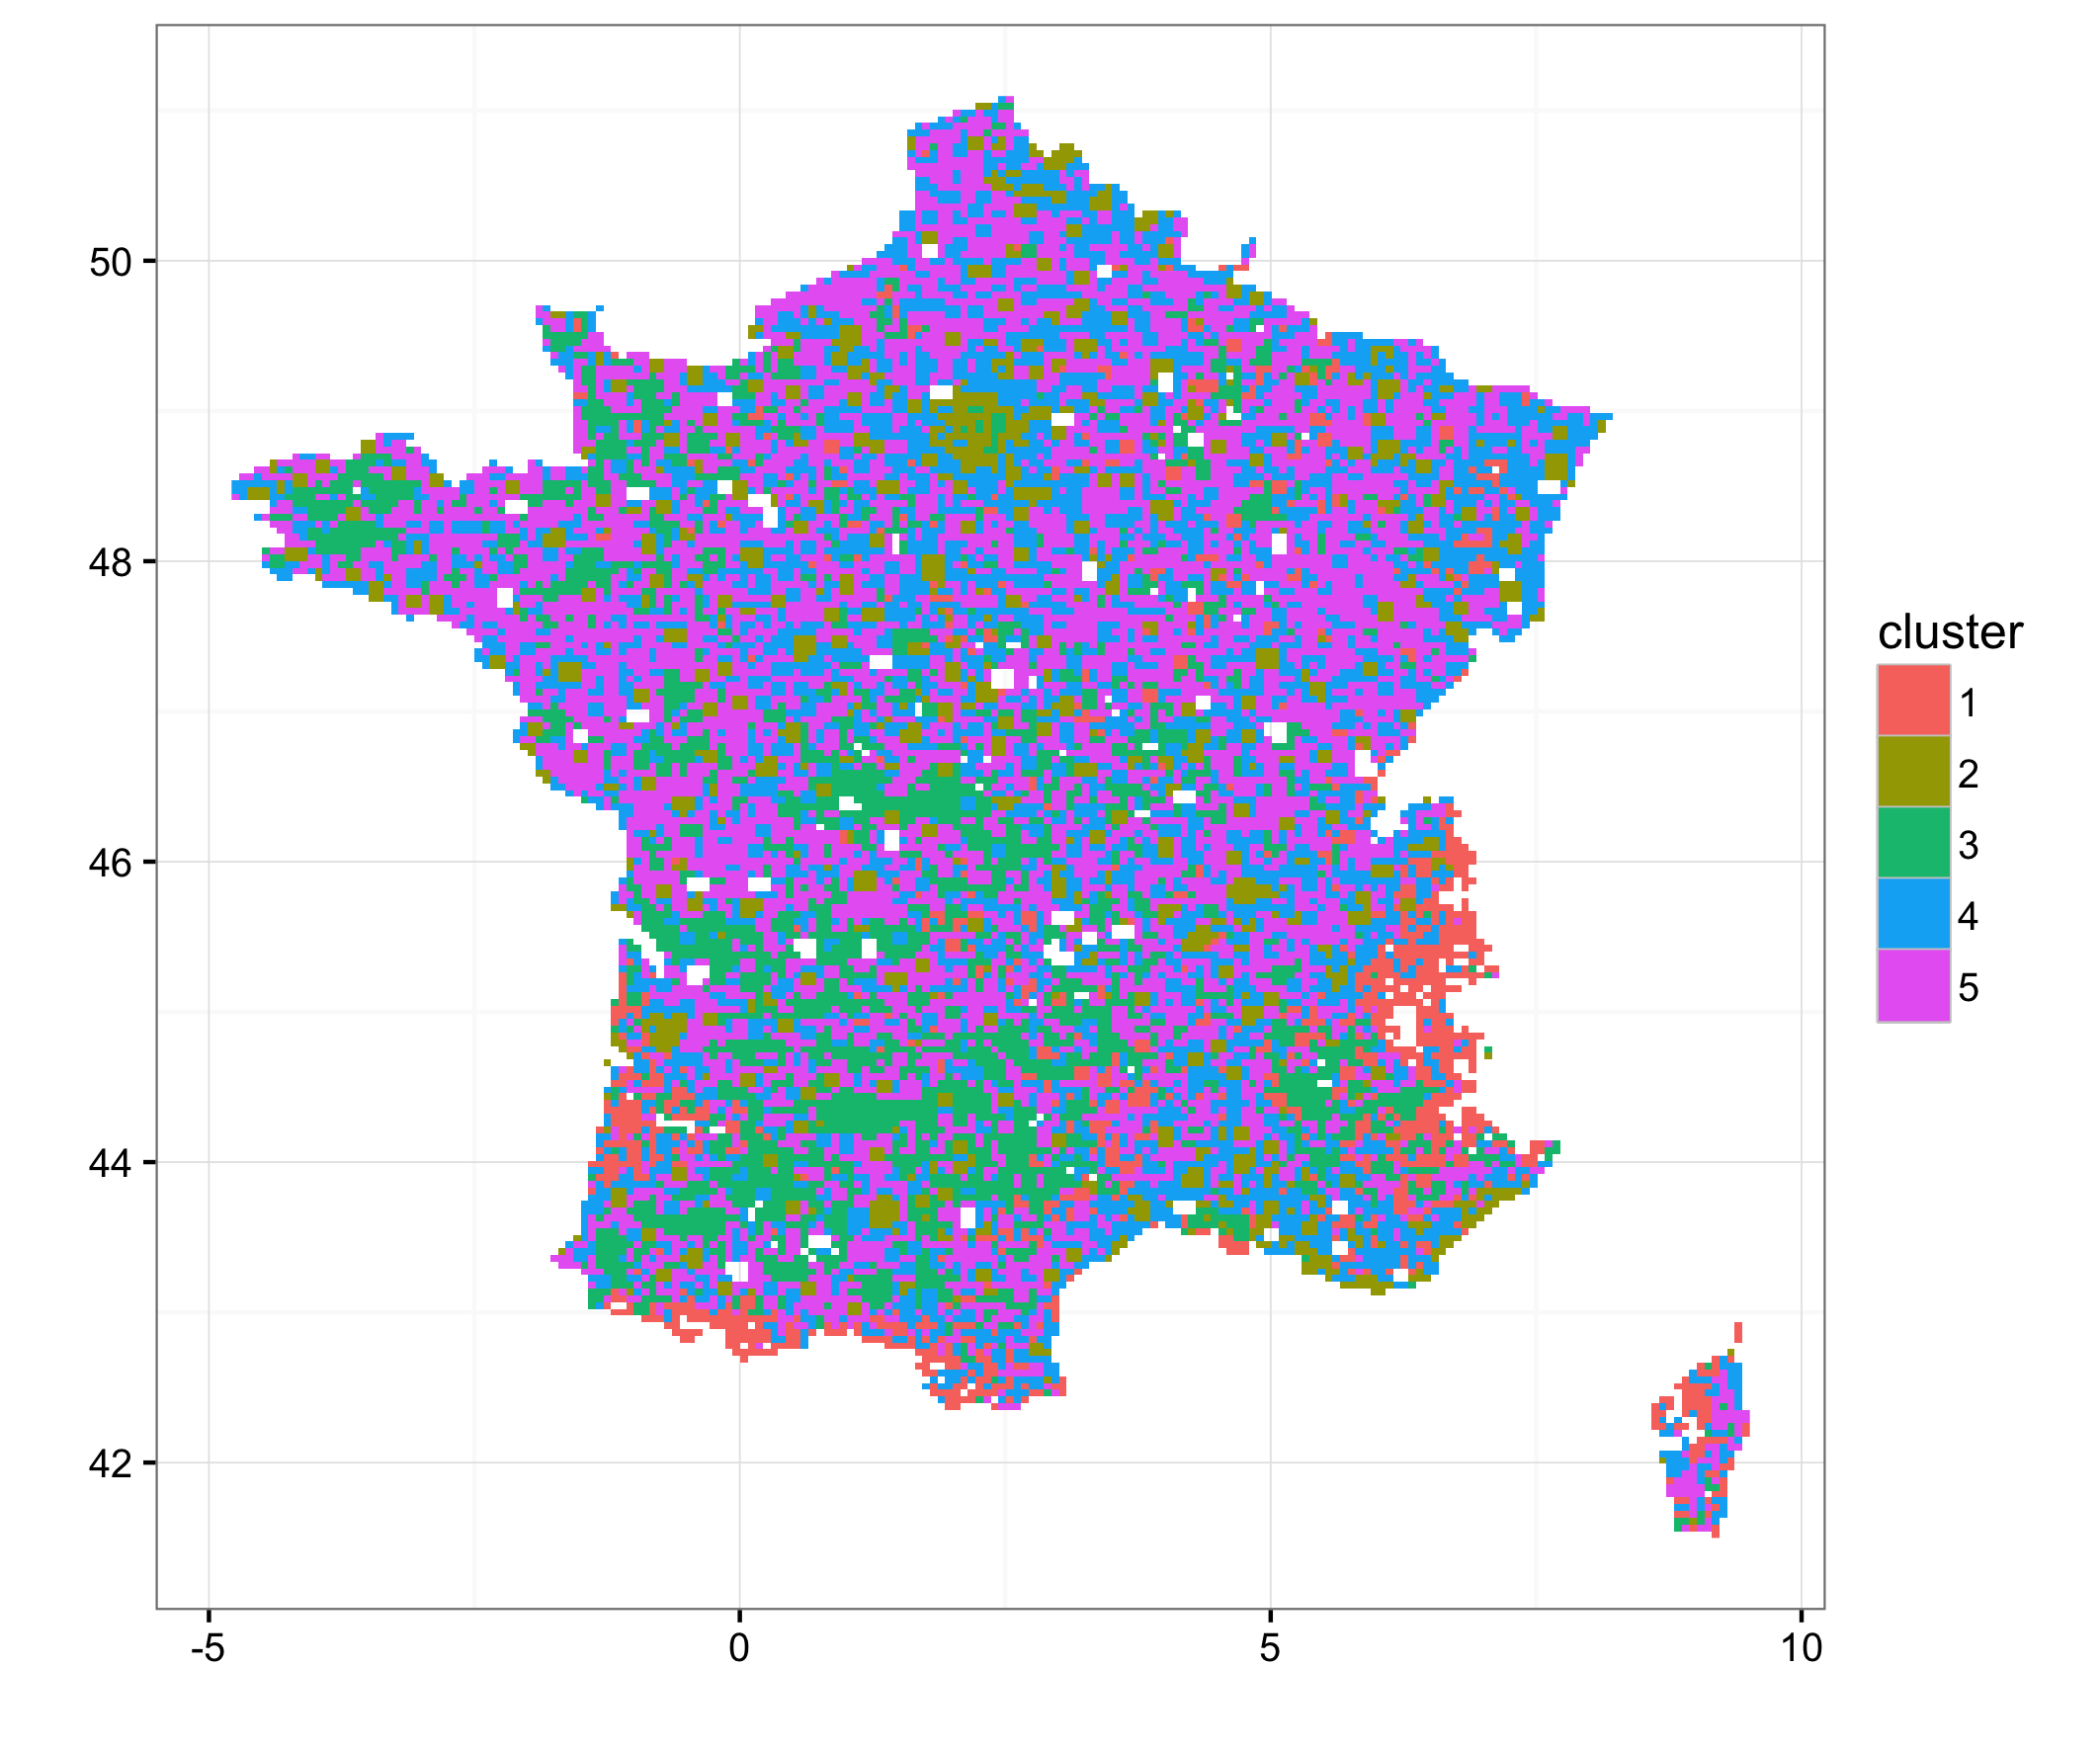
\includegraphics[width=\textwidth]{figures/density_cluster_map_k5_morpho}
%\end{columns}
%
%\justify
%
%\footnotesize\textit{Computation of morphological indicators on population density data for Europe (shown here on France), morphological classification.}
%
%}
%
%
%
%\sframe{Model Calibration}{
%
%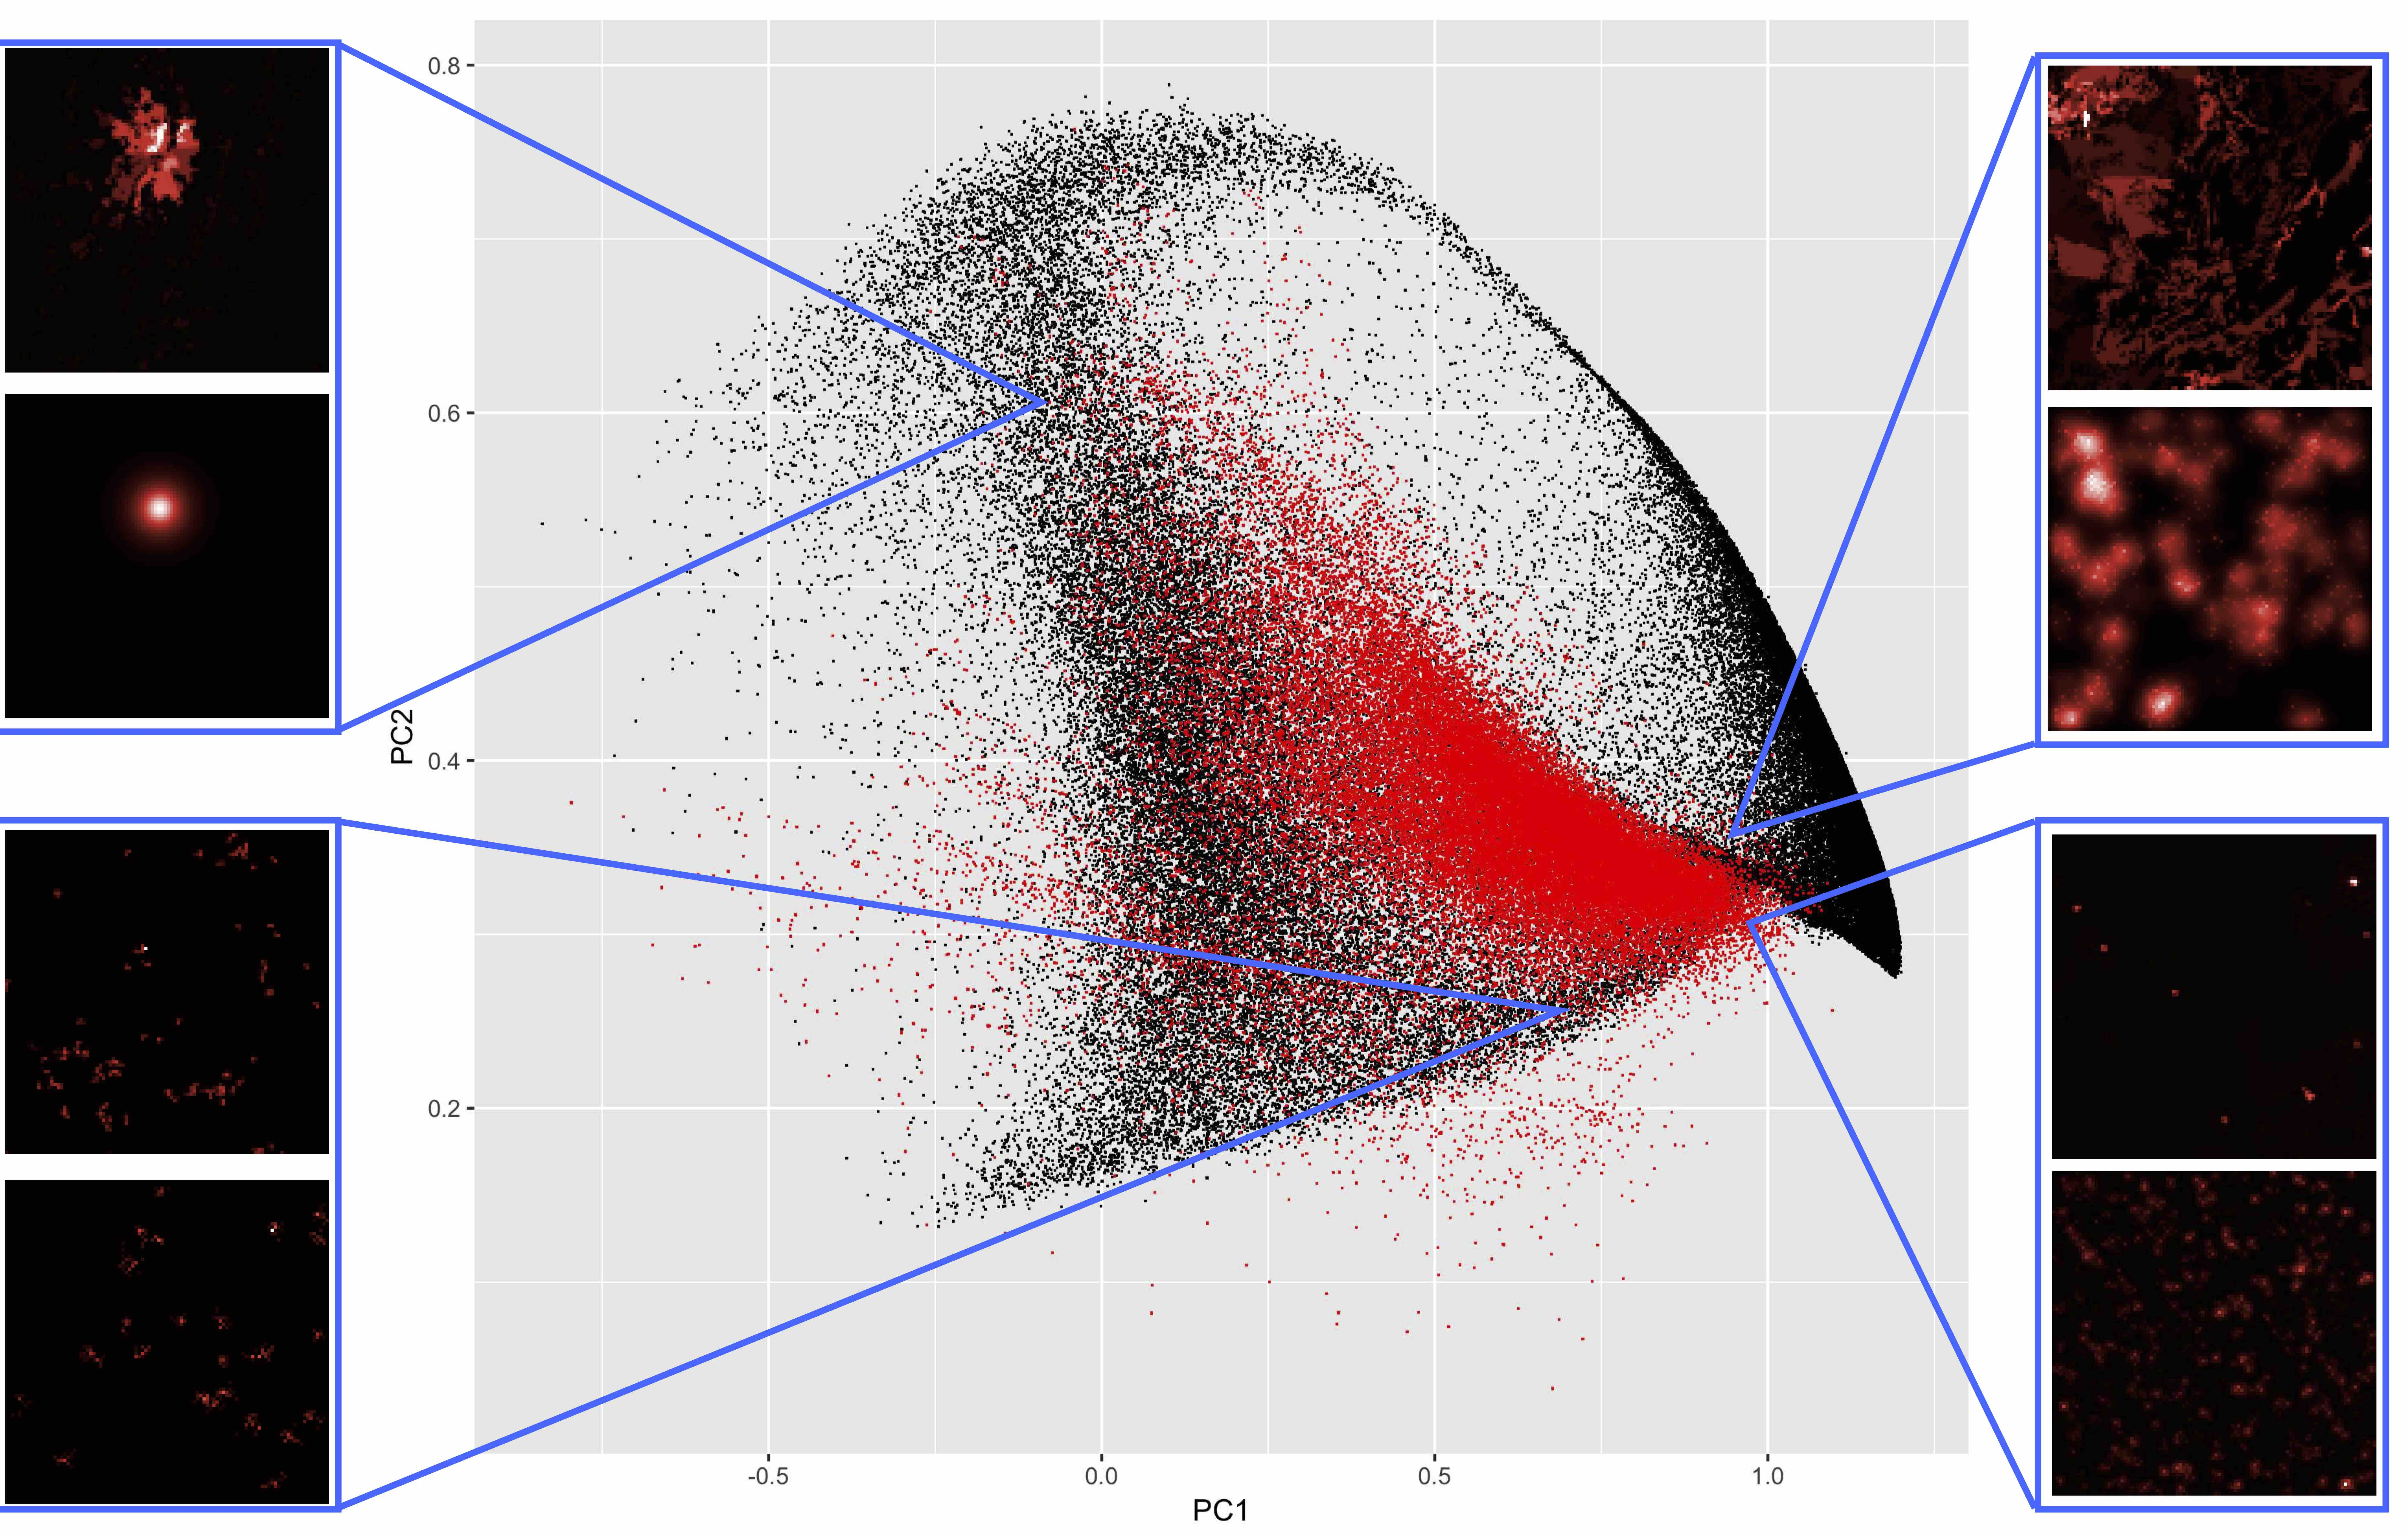
\includegraphics[width=\textwidth]{figures/density_synth}
%
%\footnotesize\textit{Brute force calibration by exploring the parameter space. Reproduction of most existing configuration in the morphological sense (here in principal plan).}
%
%}
%
%
%
%\sframe{Model Targeted Exploration}{
%
%\centering
%
%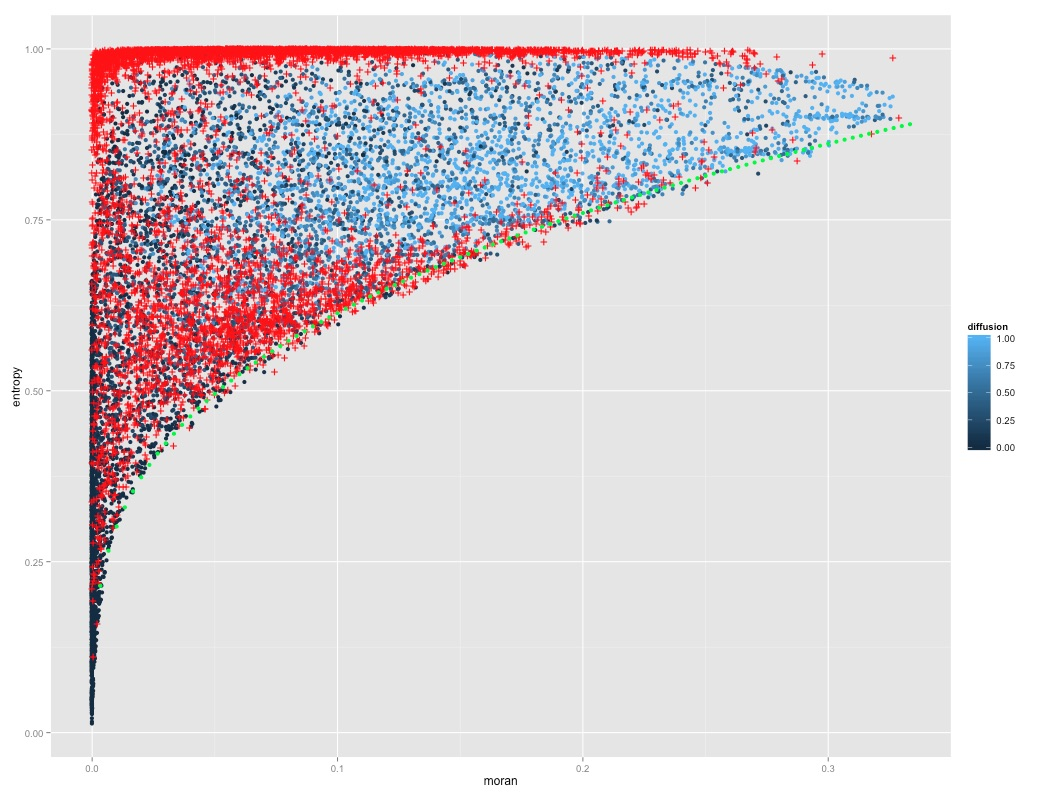
\includegraphics[width=0.8\textwidth]{figures/density_Fig6}
%
%\footnotesize\textit{Potentialities of targeted model explorations: here feasible space using Pattern Space Exploration algorithm \cite{10.1371/journal.pone.0138212}.}
%
%}
%
%
%
%
%\sframe{Including more complex processes ?}{
%
%% transition : representation of territories
%
%\textit{Which ontology to include more complex functional properties ?}
%
%\medskip
%
%$\rightarrow$ Territorial systems as the strong coupling between territories and (potential and realized) networks \cite{dupuy1987vers}.
%
%\medskip
%
%$\rightarrow$ Networks convey functional notions of centralities and accessibility, among others ; have furthermore proper topological properties.
%
%
%}
%
%
%\sframe{Interactions between Networks and Territories}{
%
%% qualitative slide
%% eventually layus on literature with the cit nw ? maybe too much
%% def. covevol : besoin coevol regimes, annexe
%% idem macrocoevol en annexe
%
%
%\textit{Complex co-evolutive processes between Territories and Transportation Networks}
%
%\medskip
%
%\centering
%
%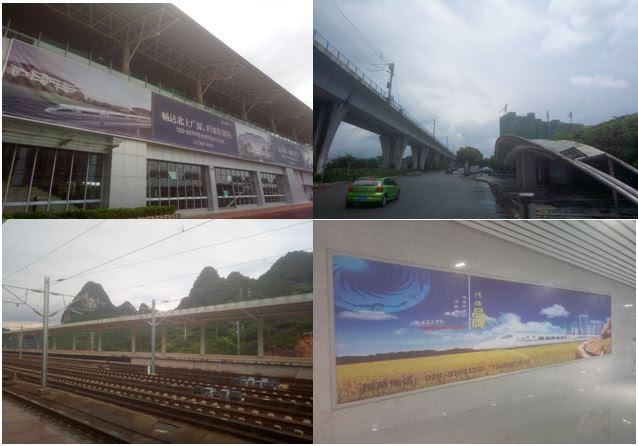
\includegraphics[height=0.7\textheight]{figures/intro_fieldwork}
%
%\footnotesize
%
%\textit{Expanding HSR network in China and ambiguous effects (Source : fieldwork survey)}
%
%
%}
%
%
%
%\sframe{A Morphogenesis Model of co-evolution}{
%
%\justify
%
%\vspace{-1cm}
%
%$\rightarrow$ Coupled grid population distribution and vector transportation network, following the core of \cite{raimbault2014hybrid}
%
%\medskip
%
%$\rightarrow$ Local morphological and functional variables determine a patch-value, driving new population attribution through preferential attachment ; combined to population diffusion (reaction-diffusion processes studied before)
%
%% Comment Arnaud : réaction-diffusion ?
%
%\medskip
%
%$\rightarrow$ Network growth is also driven by morphological, functional and local network measures, following diverse heuristics corresponding to different processes (multi-modeling)
%
%\bigskip
%\bigskip
%
%\textit{Local variables and network properties induce feedback on both, thus a strong coupling capturing the \textbf{co-evolution}}
%
%}
%
%
%
%\sframe{Model : Specification}{
%
%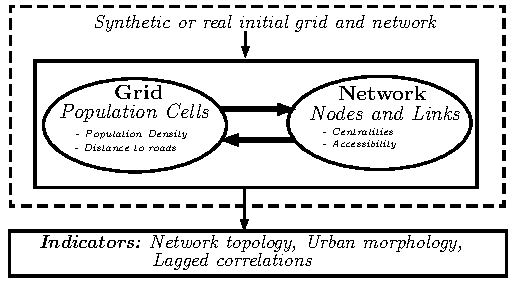
\includegraphics[width=\textwidth]{figures/coevol_mesocoevol}
%
%}
%
%
%
%\sframe{Network Generation}{
%
%At fixed time steps :
%
%\begin{enumerate}
%	\item Add new nodes preferentially to new population and connect them
%	\item \justify Variable heuristic for new links, among: nothing, random, gravity-based deterministic breakdown, gravity-based random breakdown (from \cite{schmitt2014modelisation}), cost-benefits (from \cite{louf2013emergence}), biological network generation (based on \cite{tero2010rules})
%\end{enumerate}
%
%\medskip
%
%\centering
%
%\frame{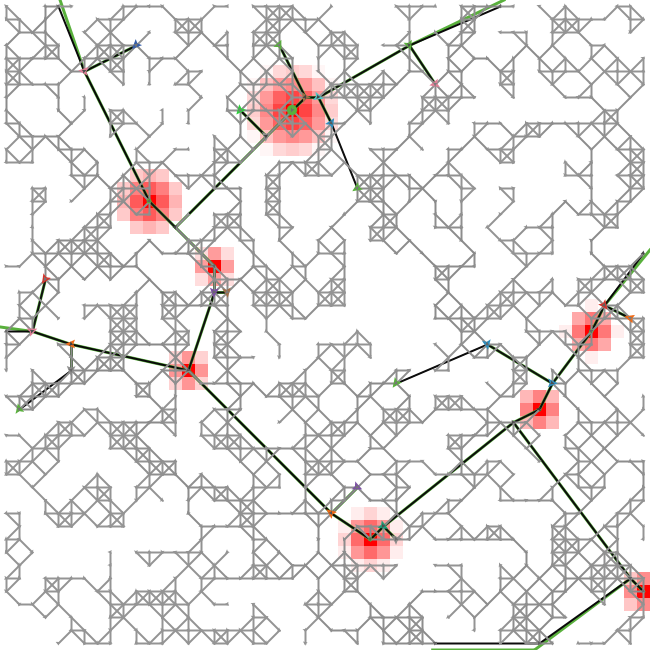
\includegraphics[height=0.31\textwidth]{figures/coevol_example-bio-process-1}}\hspace{0.2cm}
%\frame{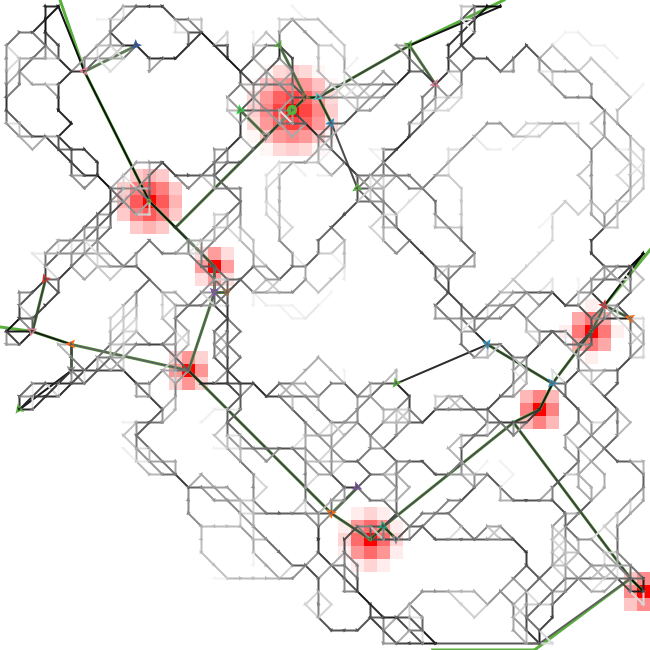
\includegraphics[height=0.31\textwidth]{figures/coevol_example-bio-process-1-tick80}}
%
%\footnotesize
%
%\textit{Intermediate stage for biological network generation}
%
%}
%
%
%
%
%\sframe{Generated Urban Shapes: Urban Form}{
%
%\centering
%
%\frame{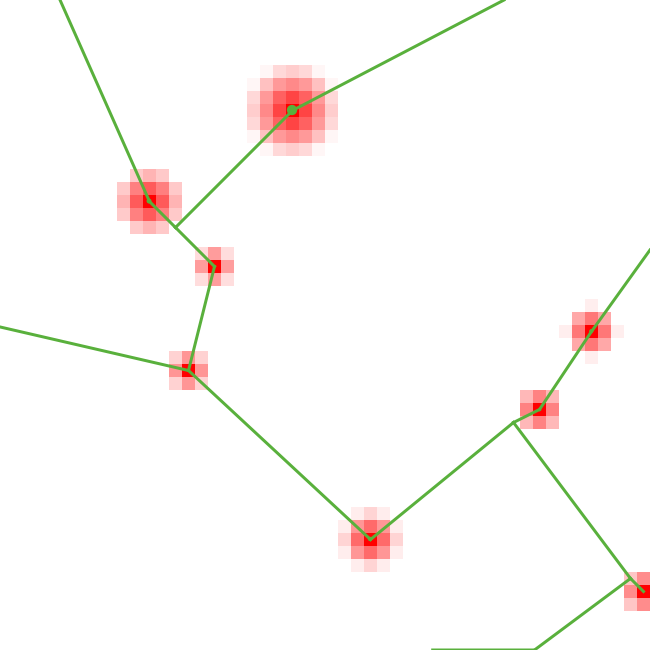
\includegraphics[width=0.28\textwidth]{figures/coevol_example_synthsetup}}\hspace{0.1cm}
%\frame{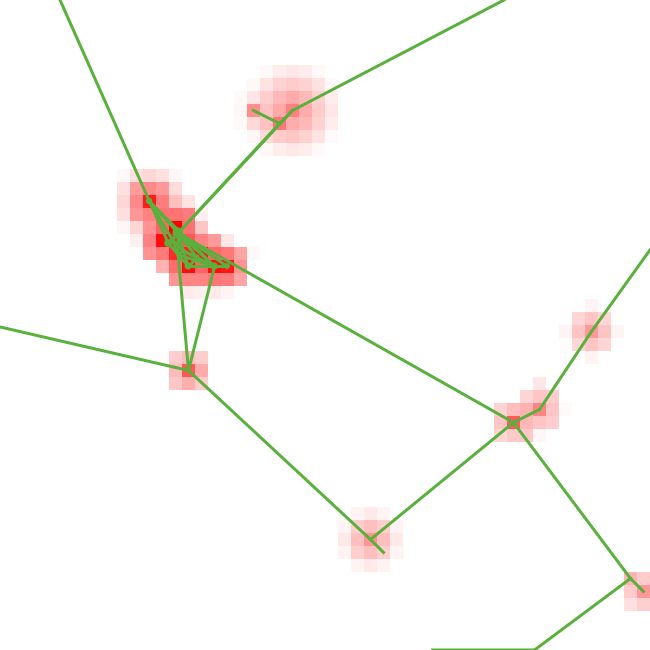
\includegraphics[width=0.28\textwidth]{figures/coevol_example_form-accessonly}}\hspace{0.1cm}
%\frame{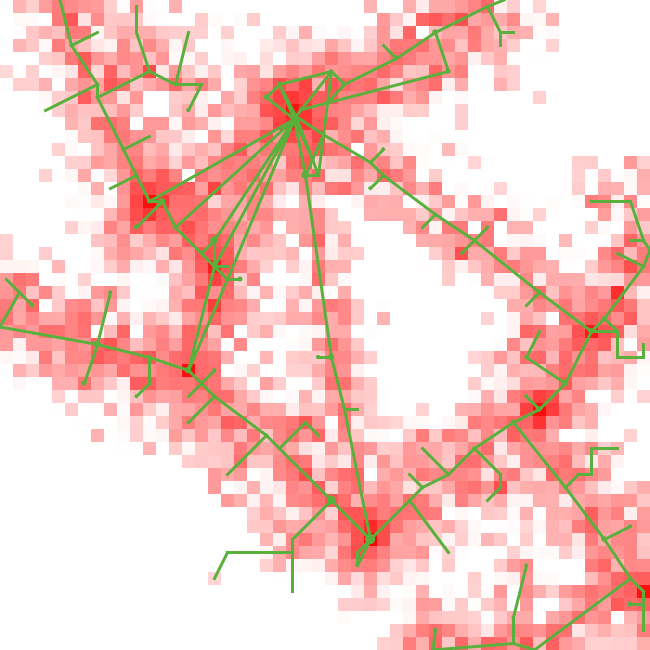
\includegraphics[width=0.28\textwidth]{figures/coevol_example_form-droadonly}}\\\vspace{0.1cm}
%\frame{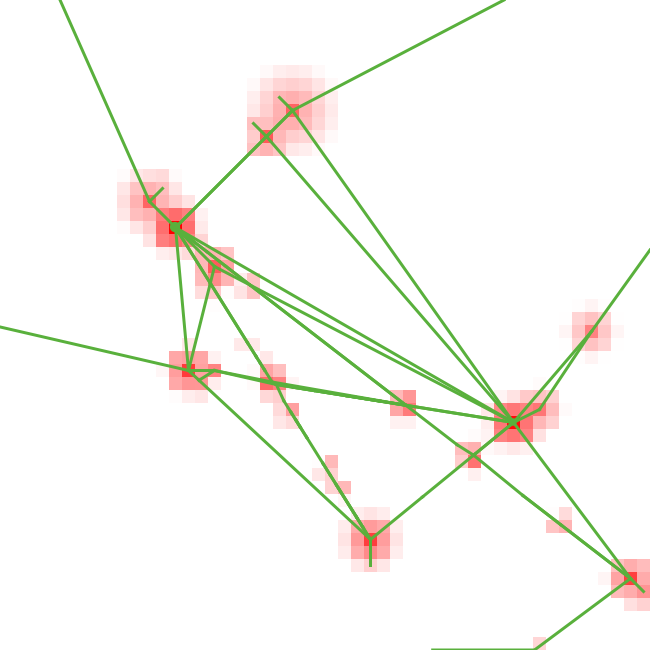
\includegraphics[width=0.28\textwidth]{figures/coevol_example_form-bwonly}}\hspace{0.1cm}
%\frame{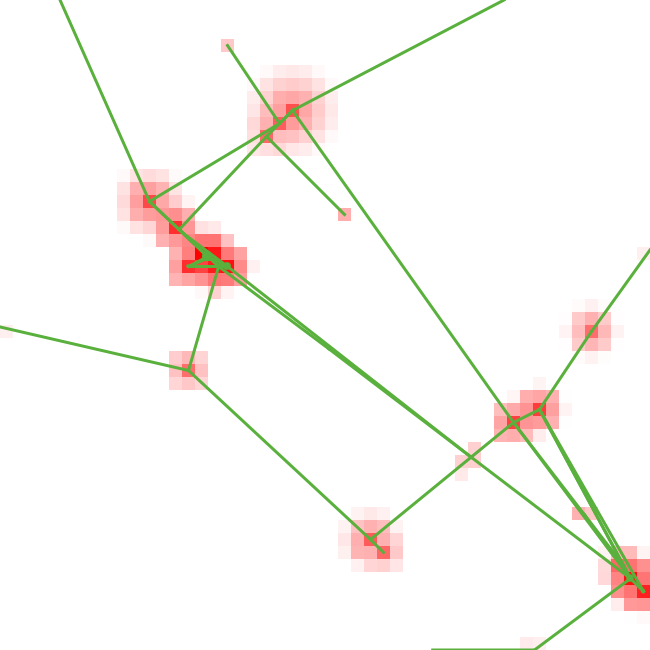
\includegraphics[width=0.28\textwidth]{figures/coevol_example_form-closenessonly}}\hspace{0.1cm}
%\frame{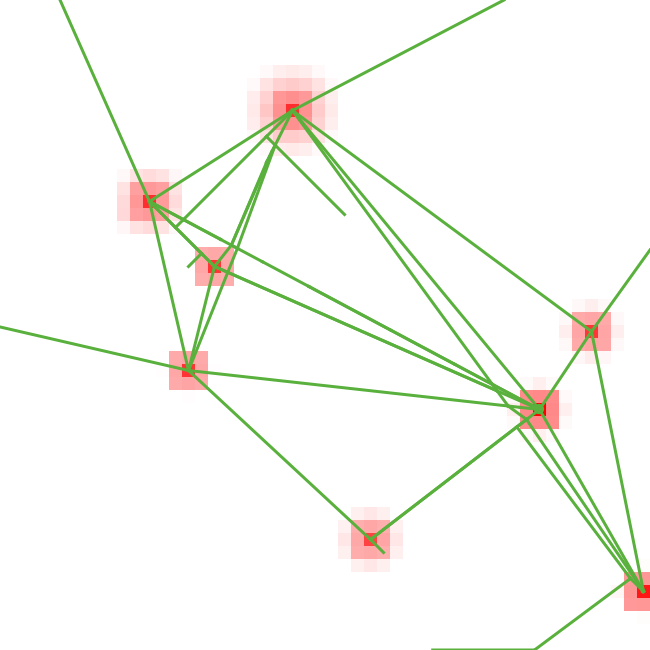
\includegraphics[width=0.28\textwidth]{figures/coevol_example_form-poponly}}
%
%\footnotesize\textit{In order: setup; accessibility driven; road distance driven; betweenness driven; closeness driven; population driven.}
%
%}
%
%
%
%
%
%
%\sframe{Generated Urban Shapes: Network}{
%
%
%\centering
%
%\frame{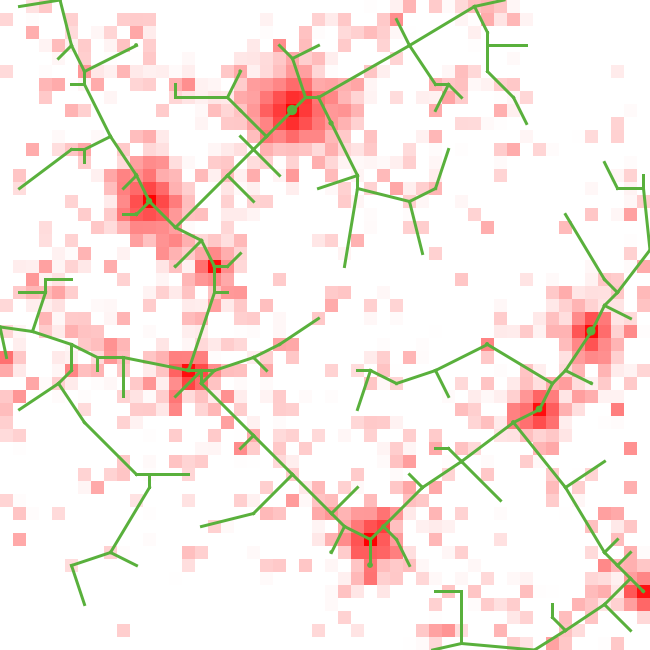
\includegraphics[width=0.28\textwidth]{figures/coevol_example_nw-connection}}\hspace{0.1cm}
%\frame{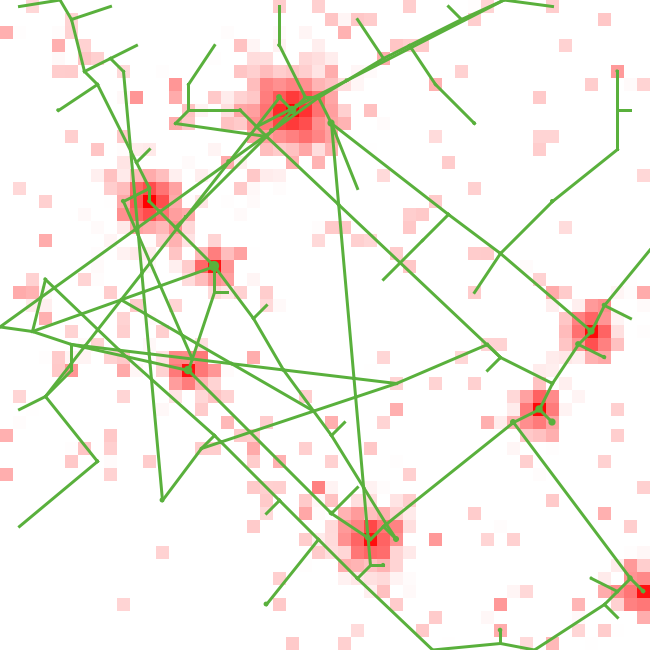
\includegraphics[width=0.28\textwidth]{figures/coevol_example_nw-random}}\hspace{0.1cm}
%\frame{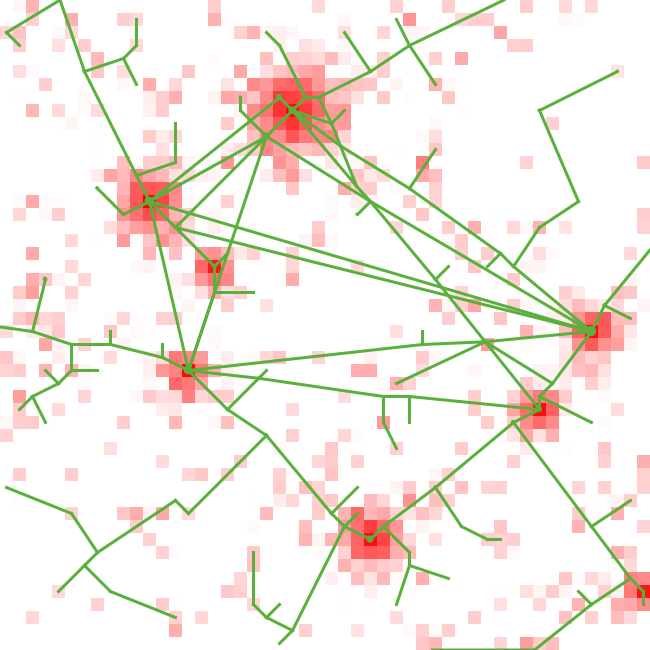
\includegraphics[width=0.28\textwidth]{figures/coevol_example_nw-gravity}}\\\vspace{0.1cm}
%\frame{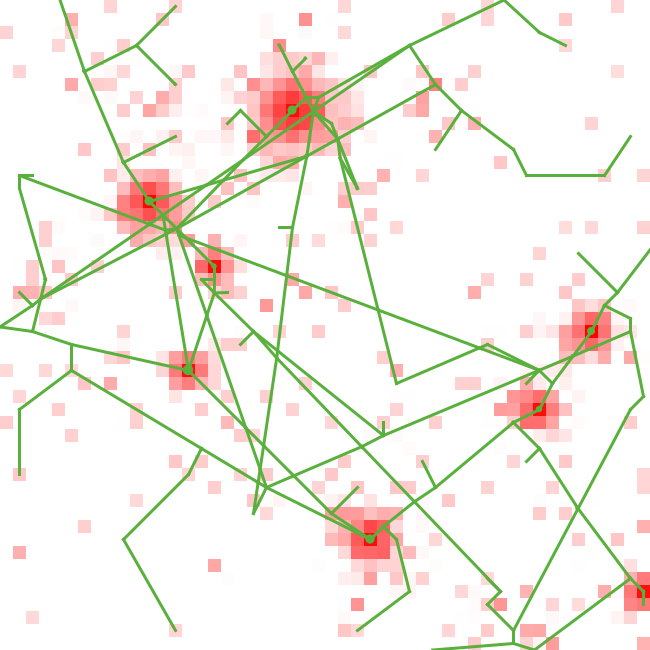
\includegraphics[width=0.28\textwidth]{figures/coevol_example_nw-rndbrkdwn}}\hspace{0.1cm}
%\frame{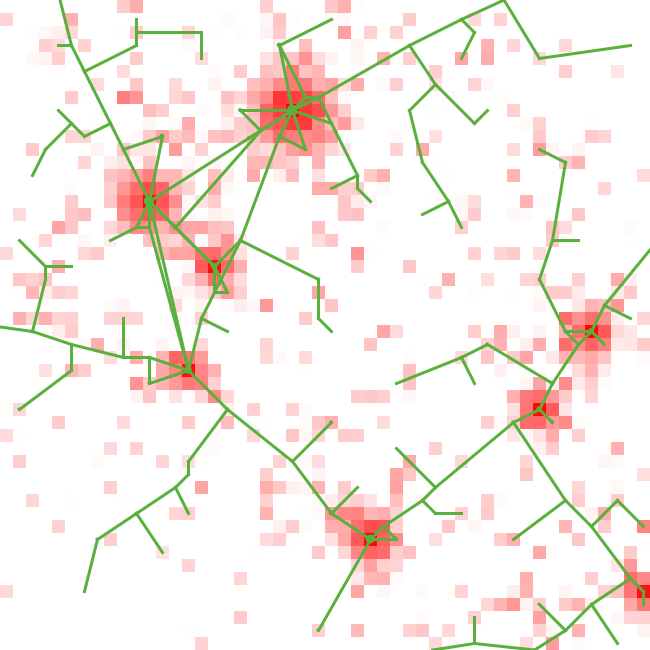
\includegraphics[width=0.28\textwidth]{figures/coevol_example_nw-cost}}\hspace{0.1cm}
%\frame{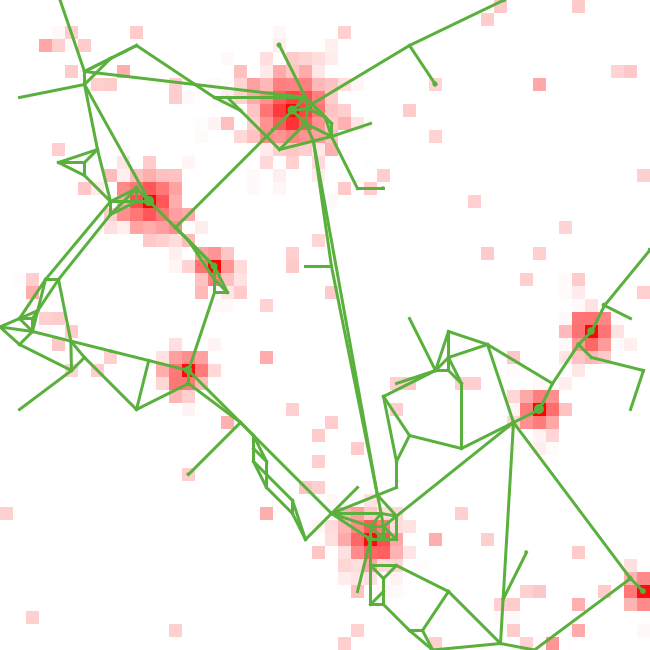
\includegraphics[width=0.28\textwidth]{figures/coevol_example_nw-bio}}
%
%\footnotesize\textit{In order: connection; random; deterministic breakdown; random breakdown; cost-driven; biological.}
%
%}
%
%
%
%\sframe{Results : Network Heuristics}{
%
%\justify
%
%\textit{Comparison of feasible space for network indicators with fixed density}
%
%\bigskip
%
%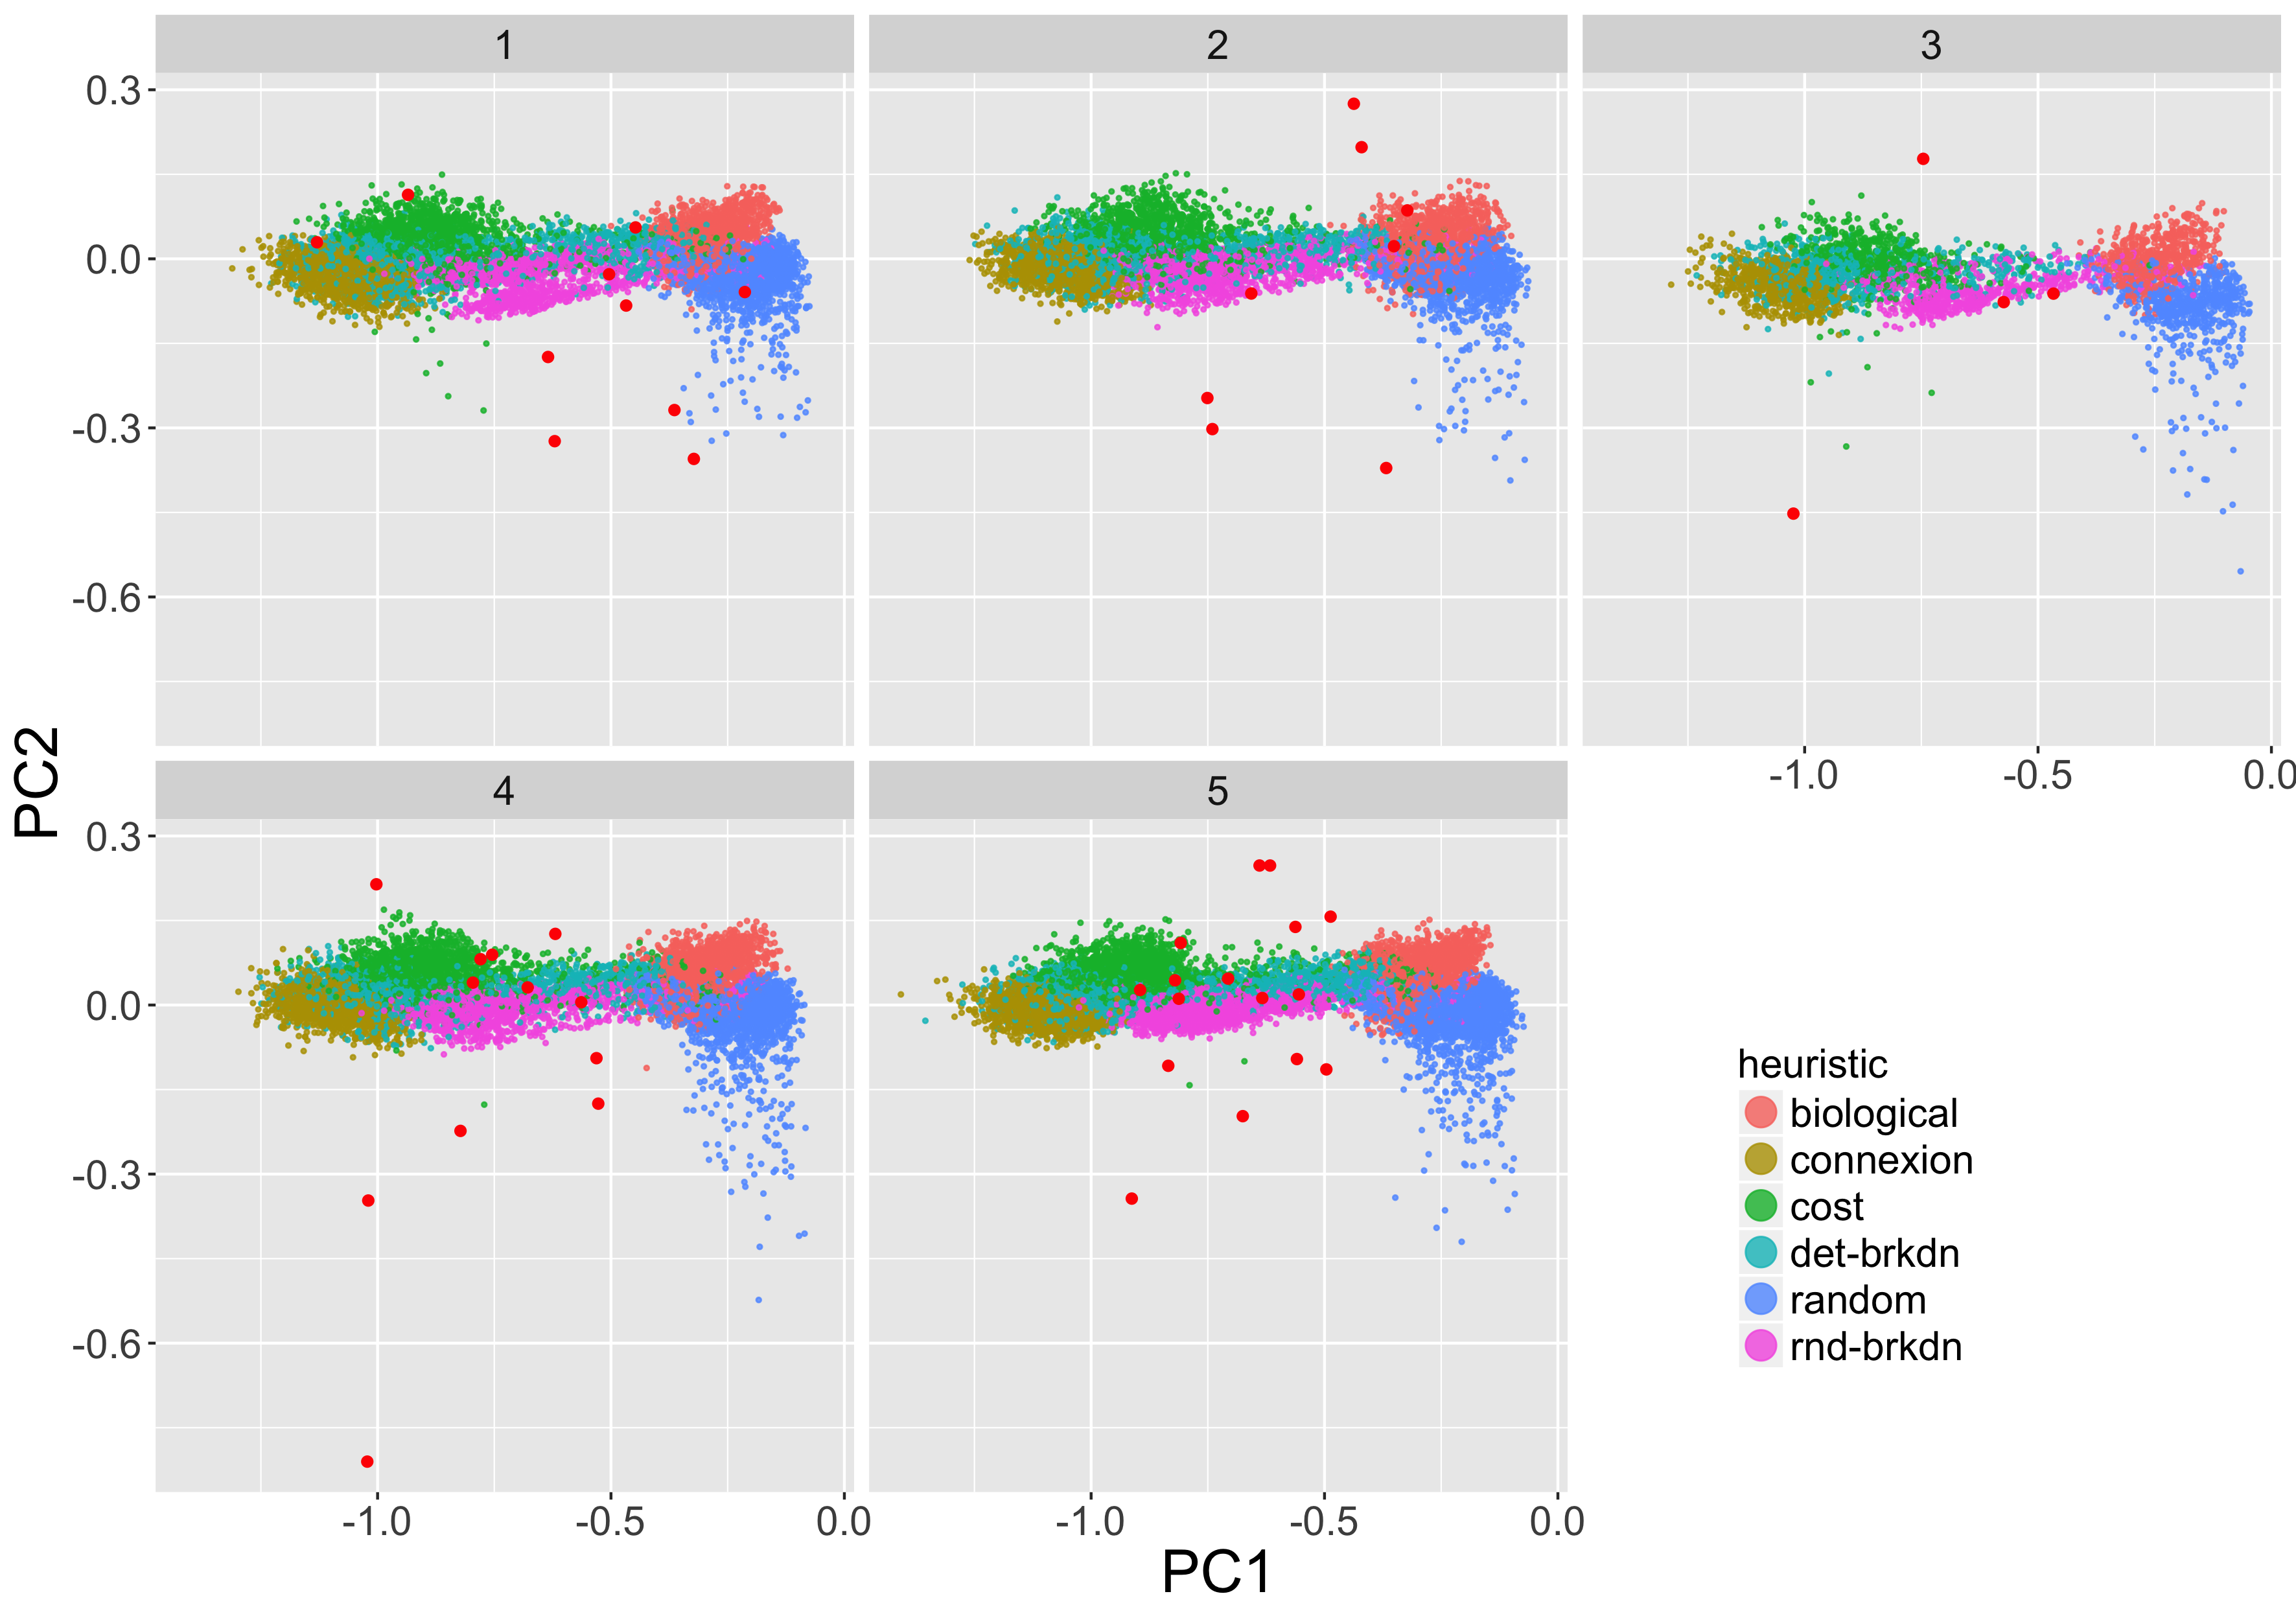
\includegraphics[width=0.52\textwidth,height=0.6\textheight]{figures/coevol_feasible_space_withreal_pca_bymorph}
%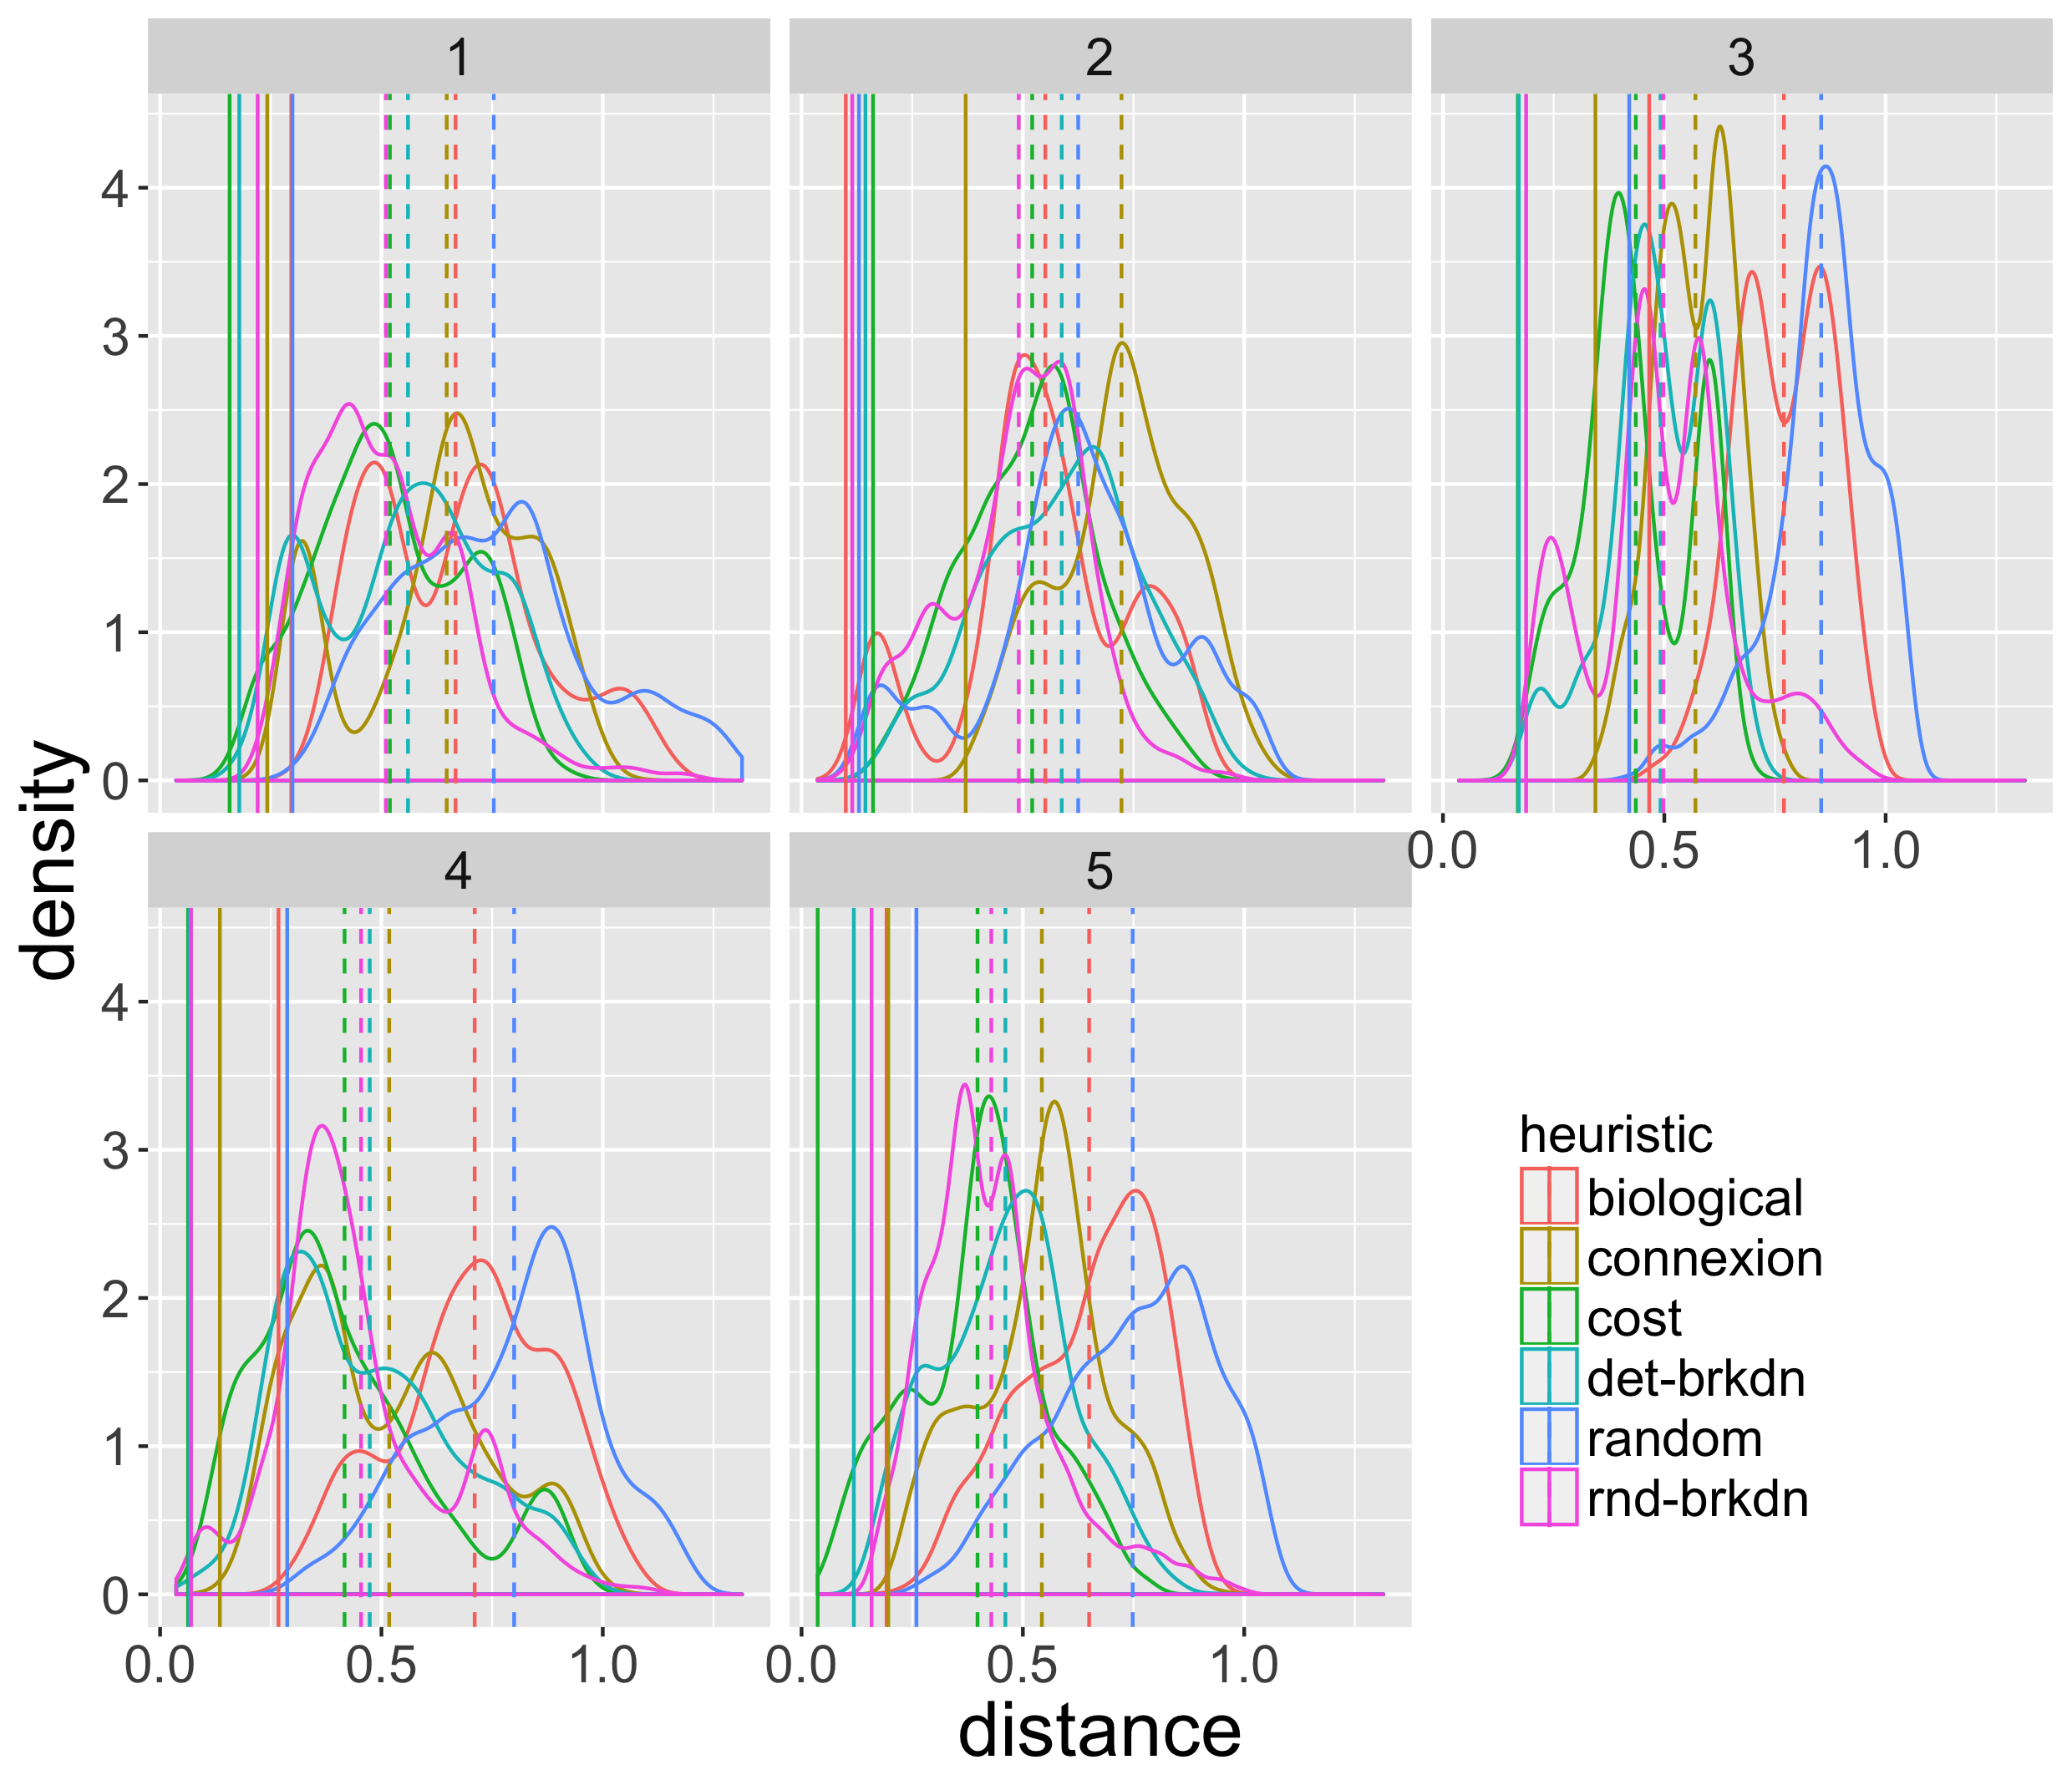
\includegraphics[width=0.43\textwidth,height=0.6\textheight]{figures/coevol_distance_real_bymorph}
%
%\footnotesize
%
%\textit{(Left) Feasible spaces by morphological class and network heuristic; (Right) Distribution of distances to topologies of real networks}
%
%}
%
%
%\sframe{Results : Calibration}{
%
%\justify
%
%\vspace{-0.5cm}
%
%Calibration (model explored with OpenMole~\cite{reuillon2013openmole}, $\sim 10^6$ model runs) at the first order on morphological and topological objectives, and on correlations matrices.
%
%\bigskip
%
%\begin{columns}
%\column{0.4\textwidth}
%\centering
%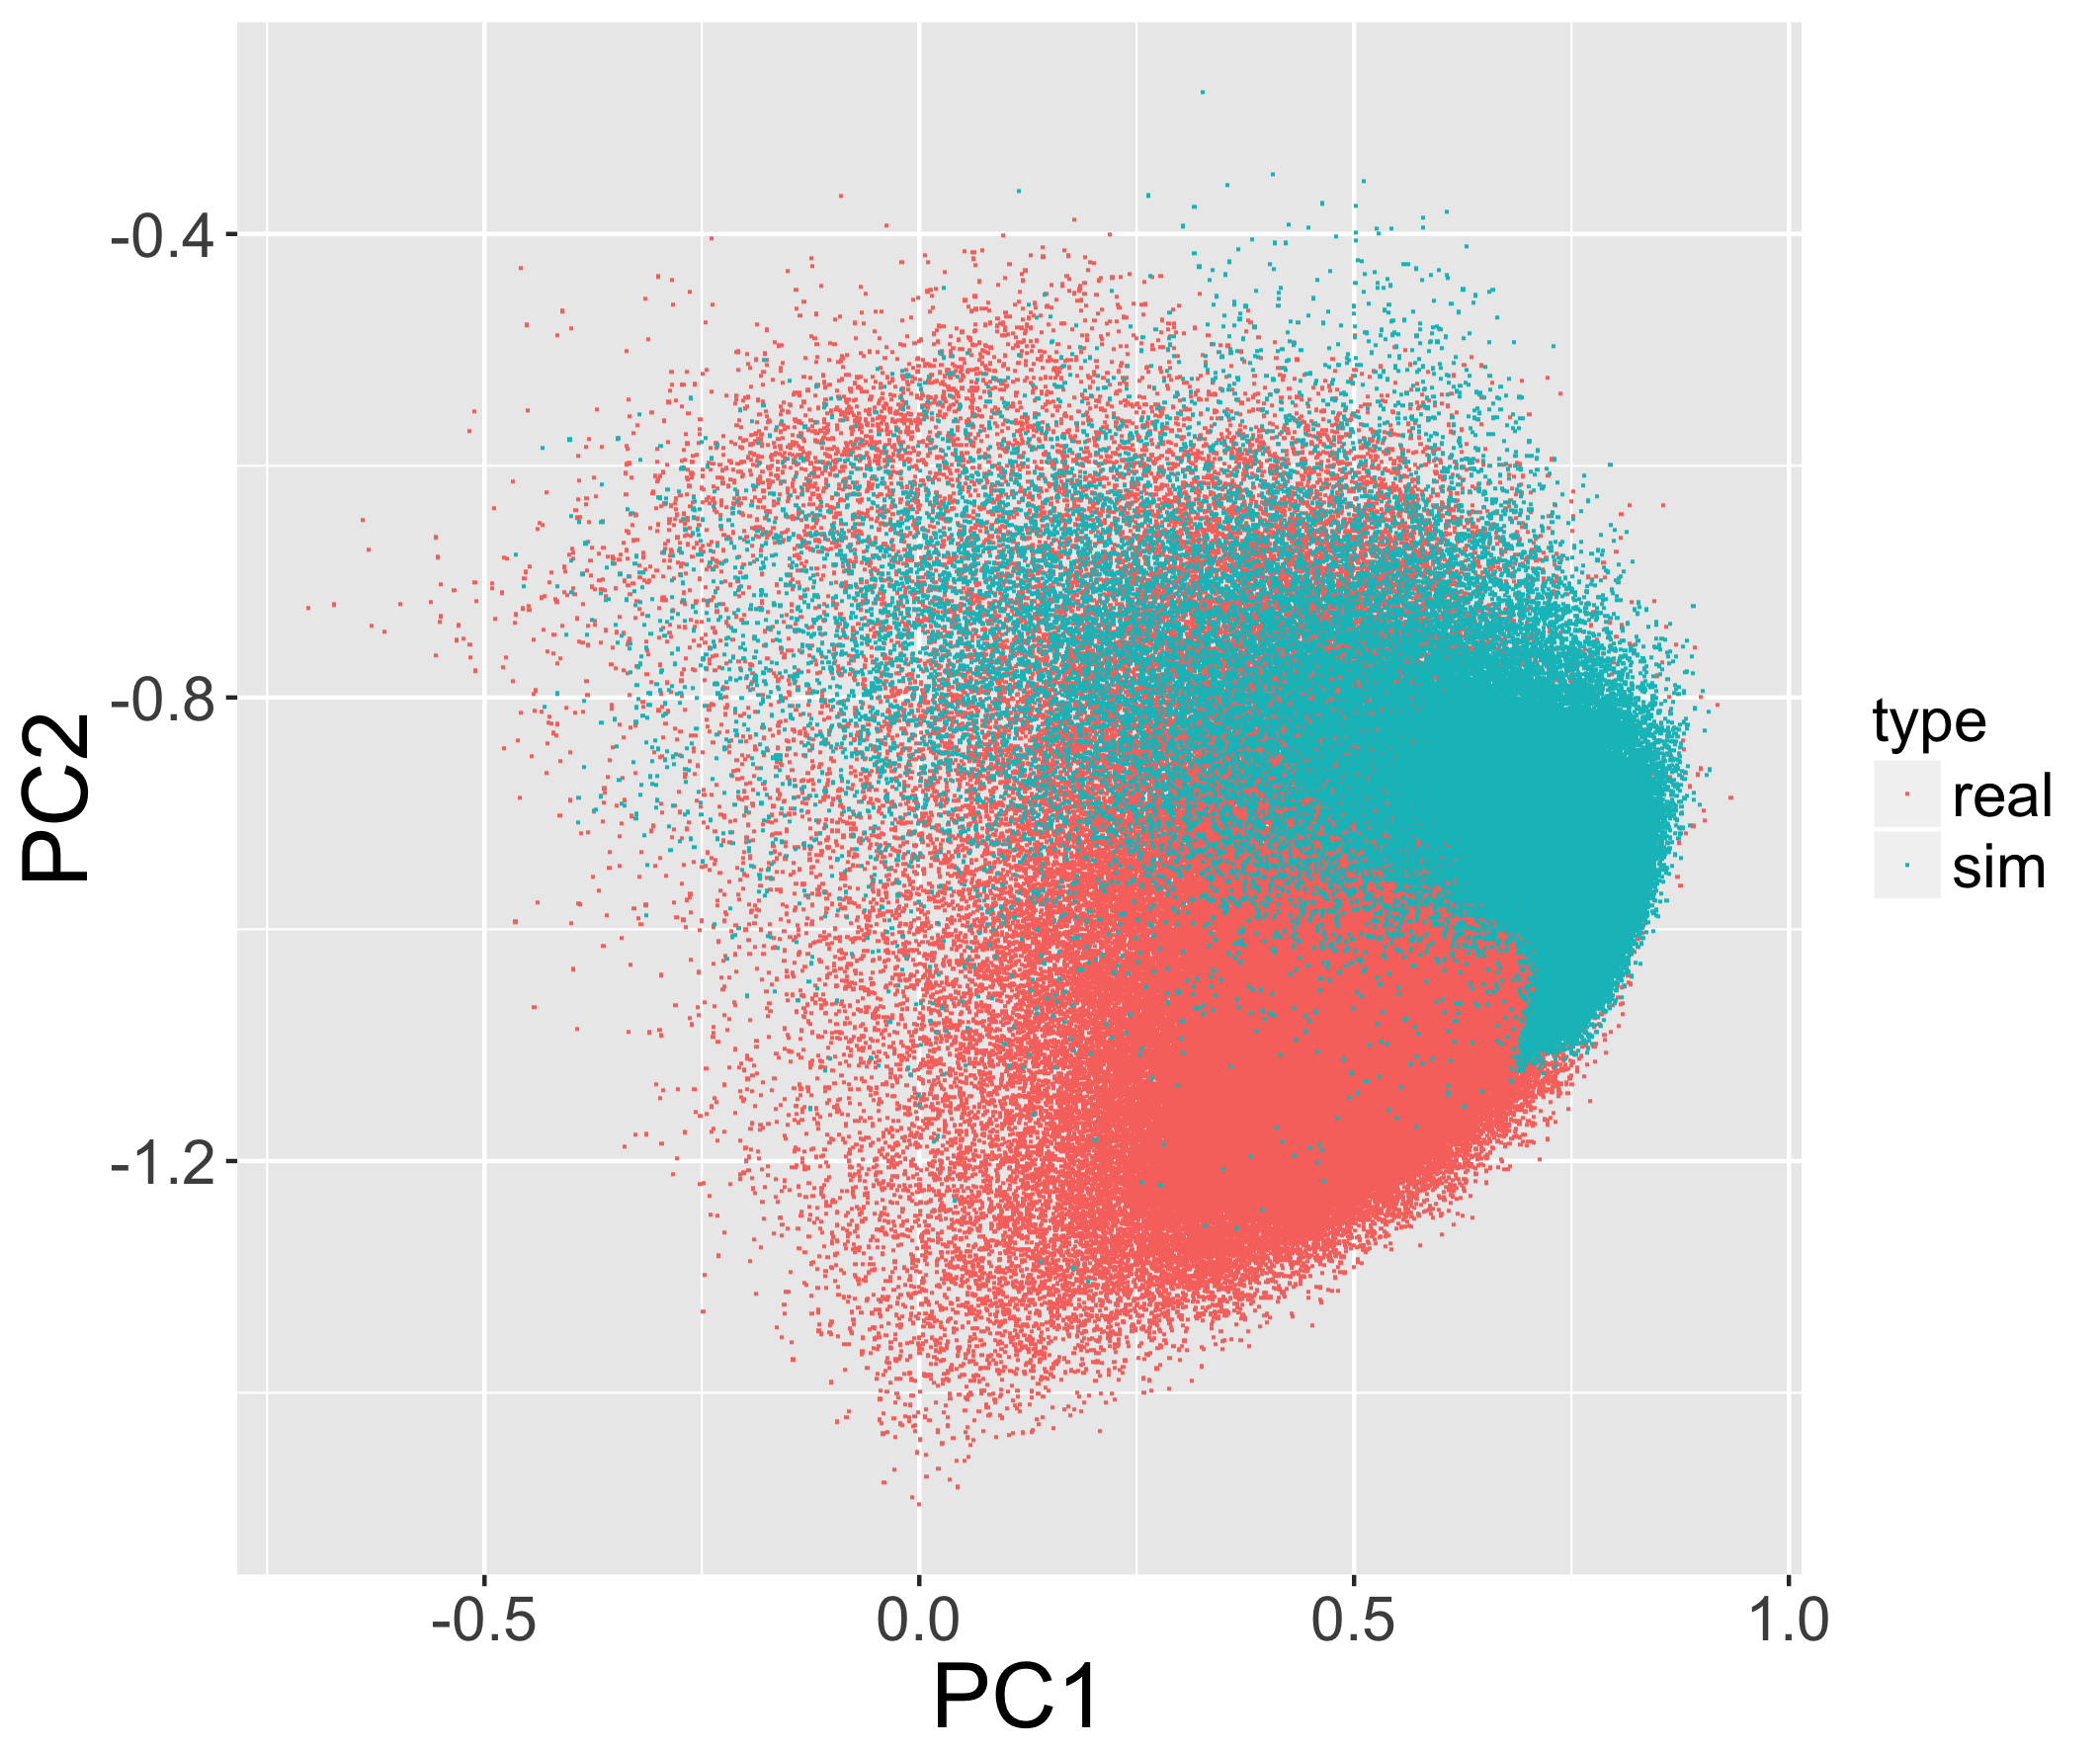
\includegraphics[width=\textwidth]{figures/coevol_pca_allobjs}
%\column{0.2\textwidth}
%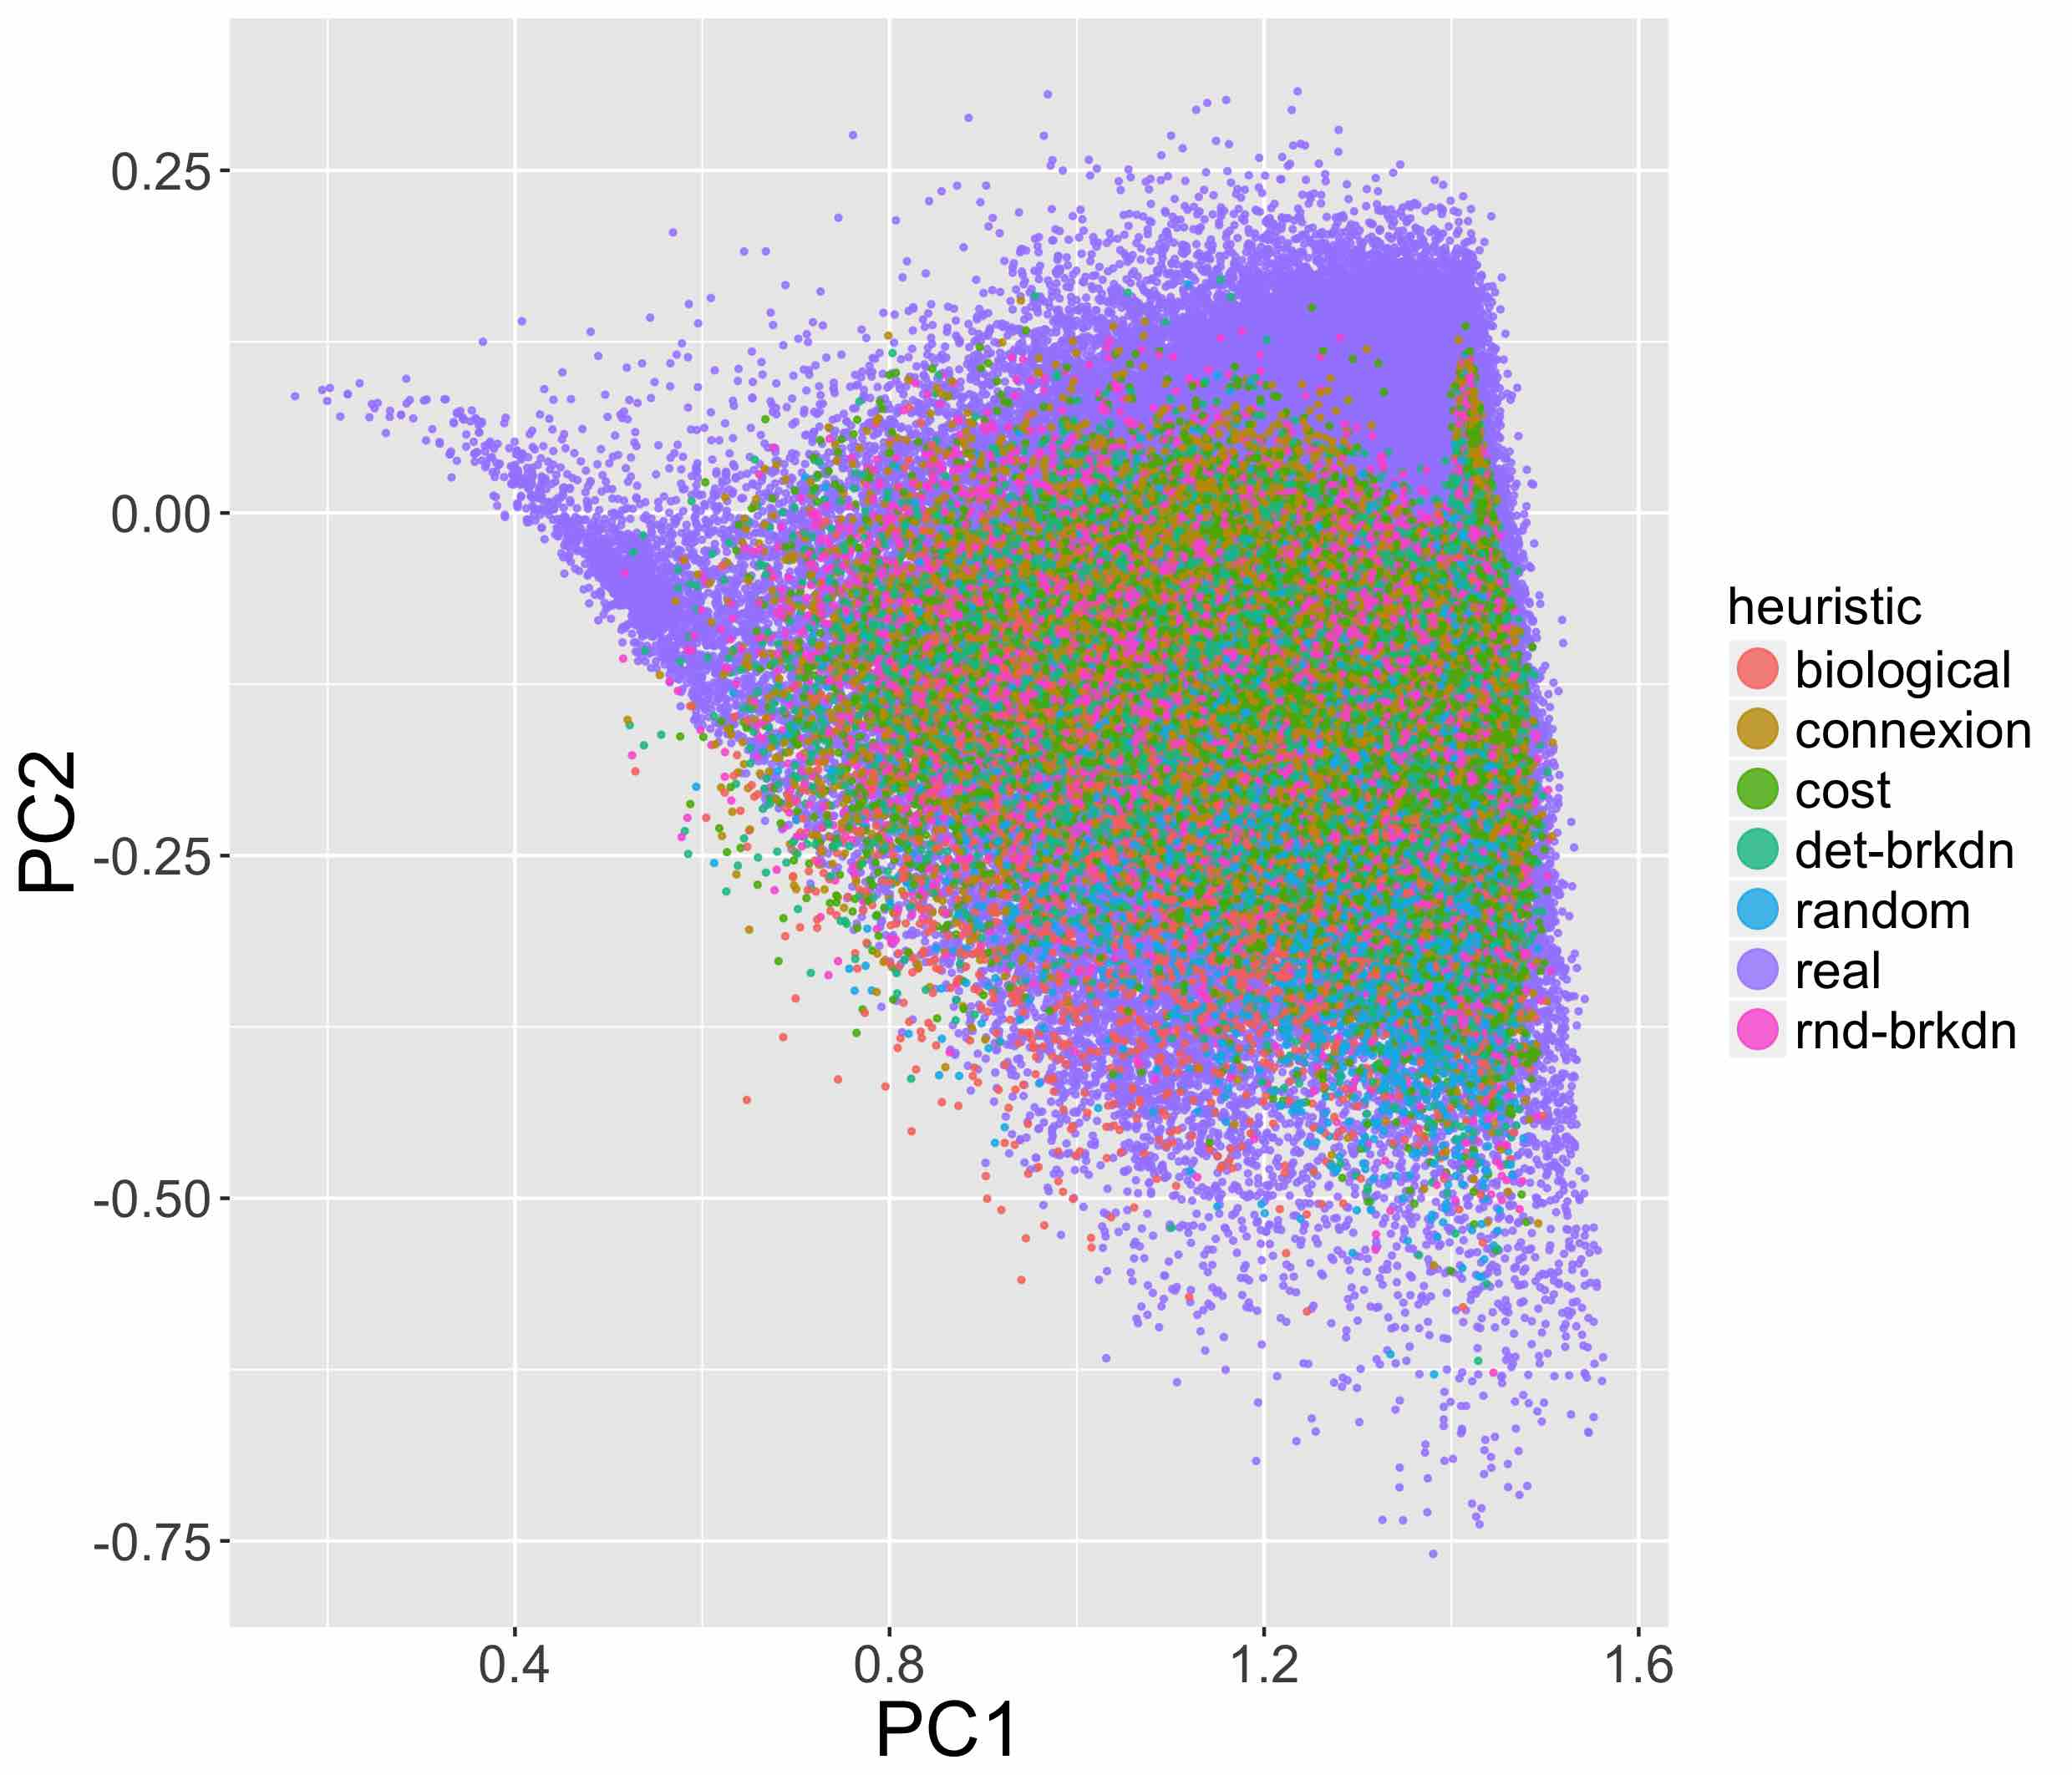
\includegraphics[width=\textwidth]{figures/coevol_pca_morpho_byheuristic}\\
%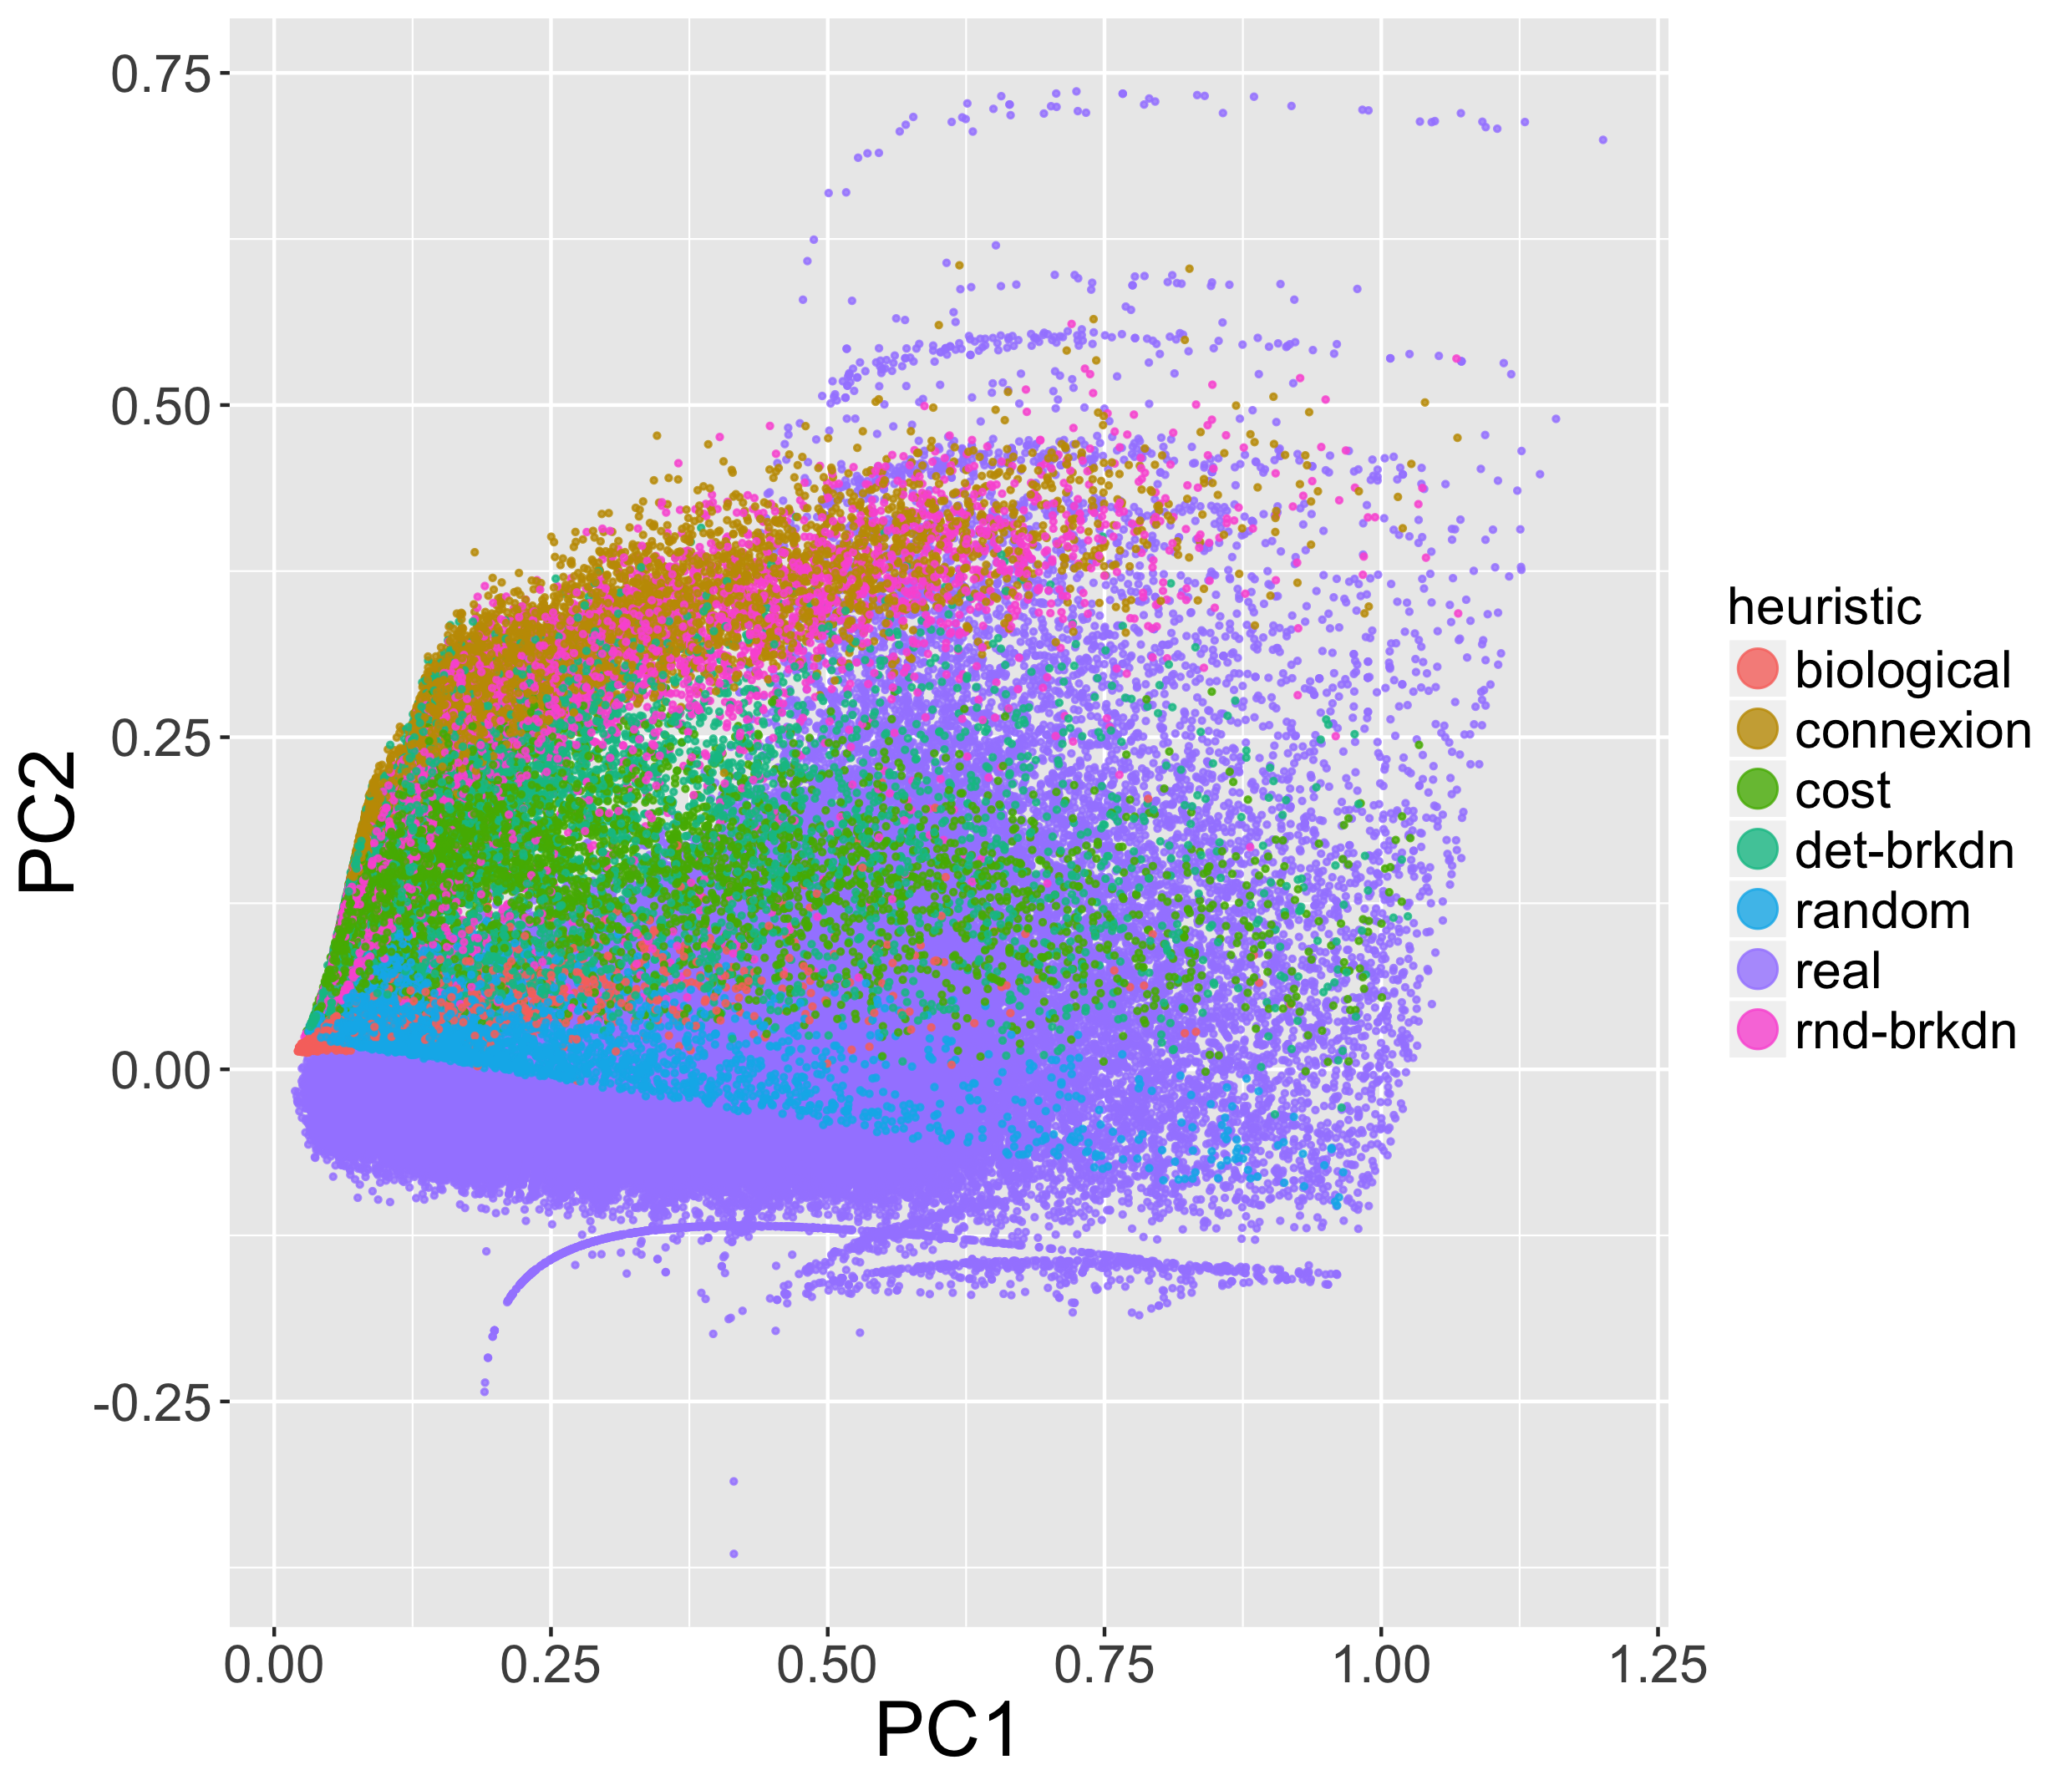
\includegraphics[width=\textwidth]{figures/coevol_pca_network_byheuristic}
%\column{0.4\textwidth}
%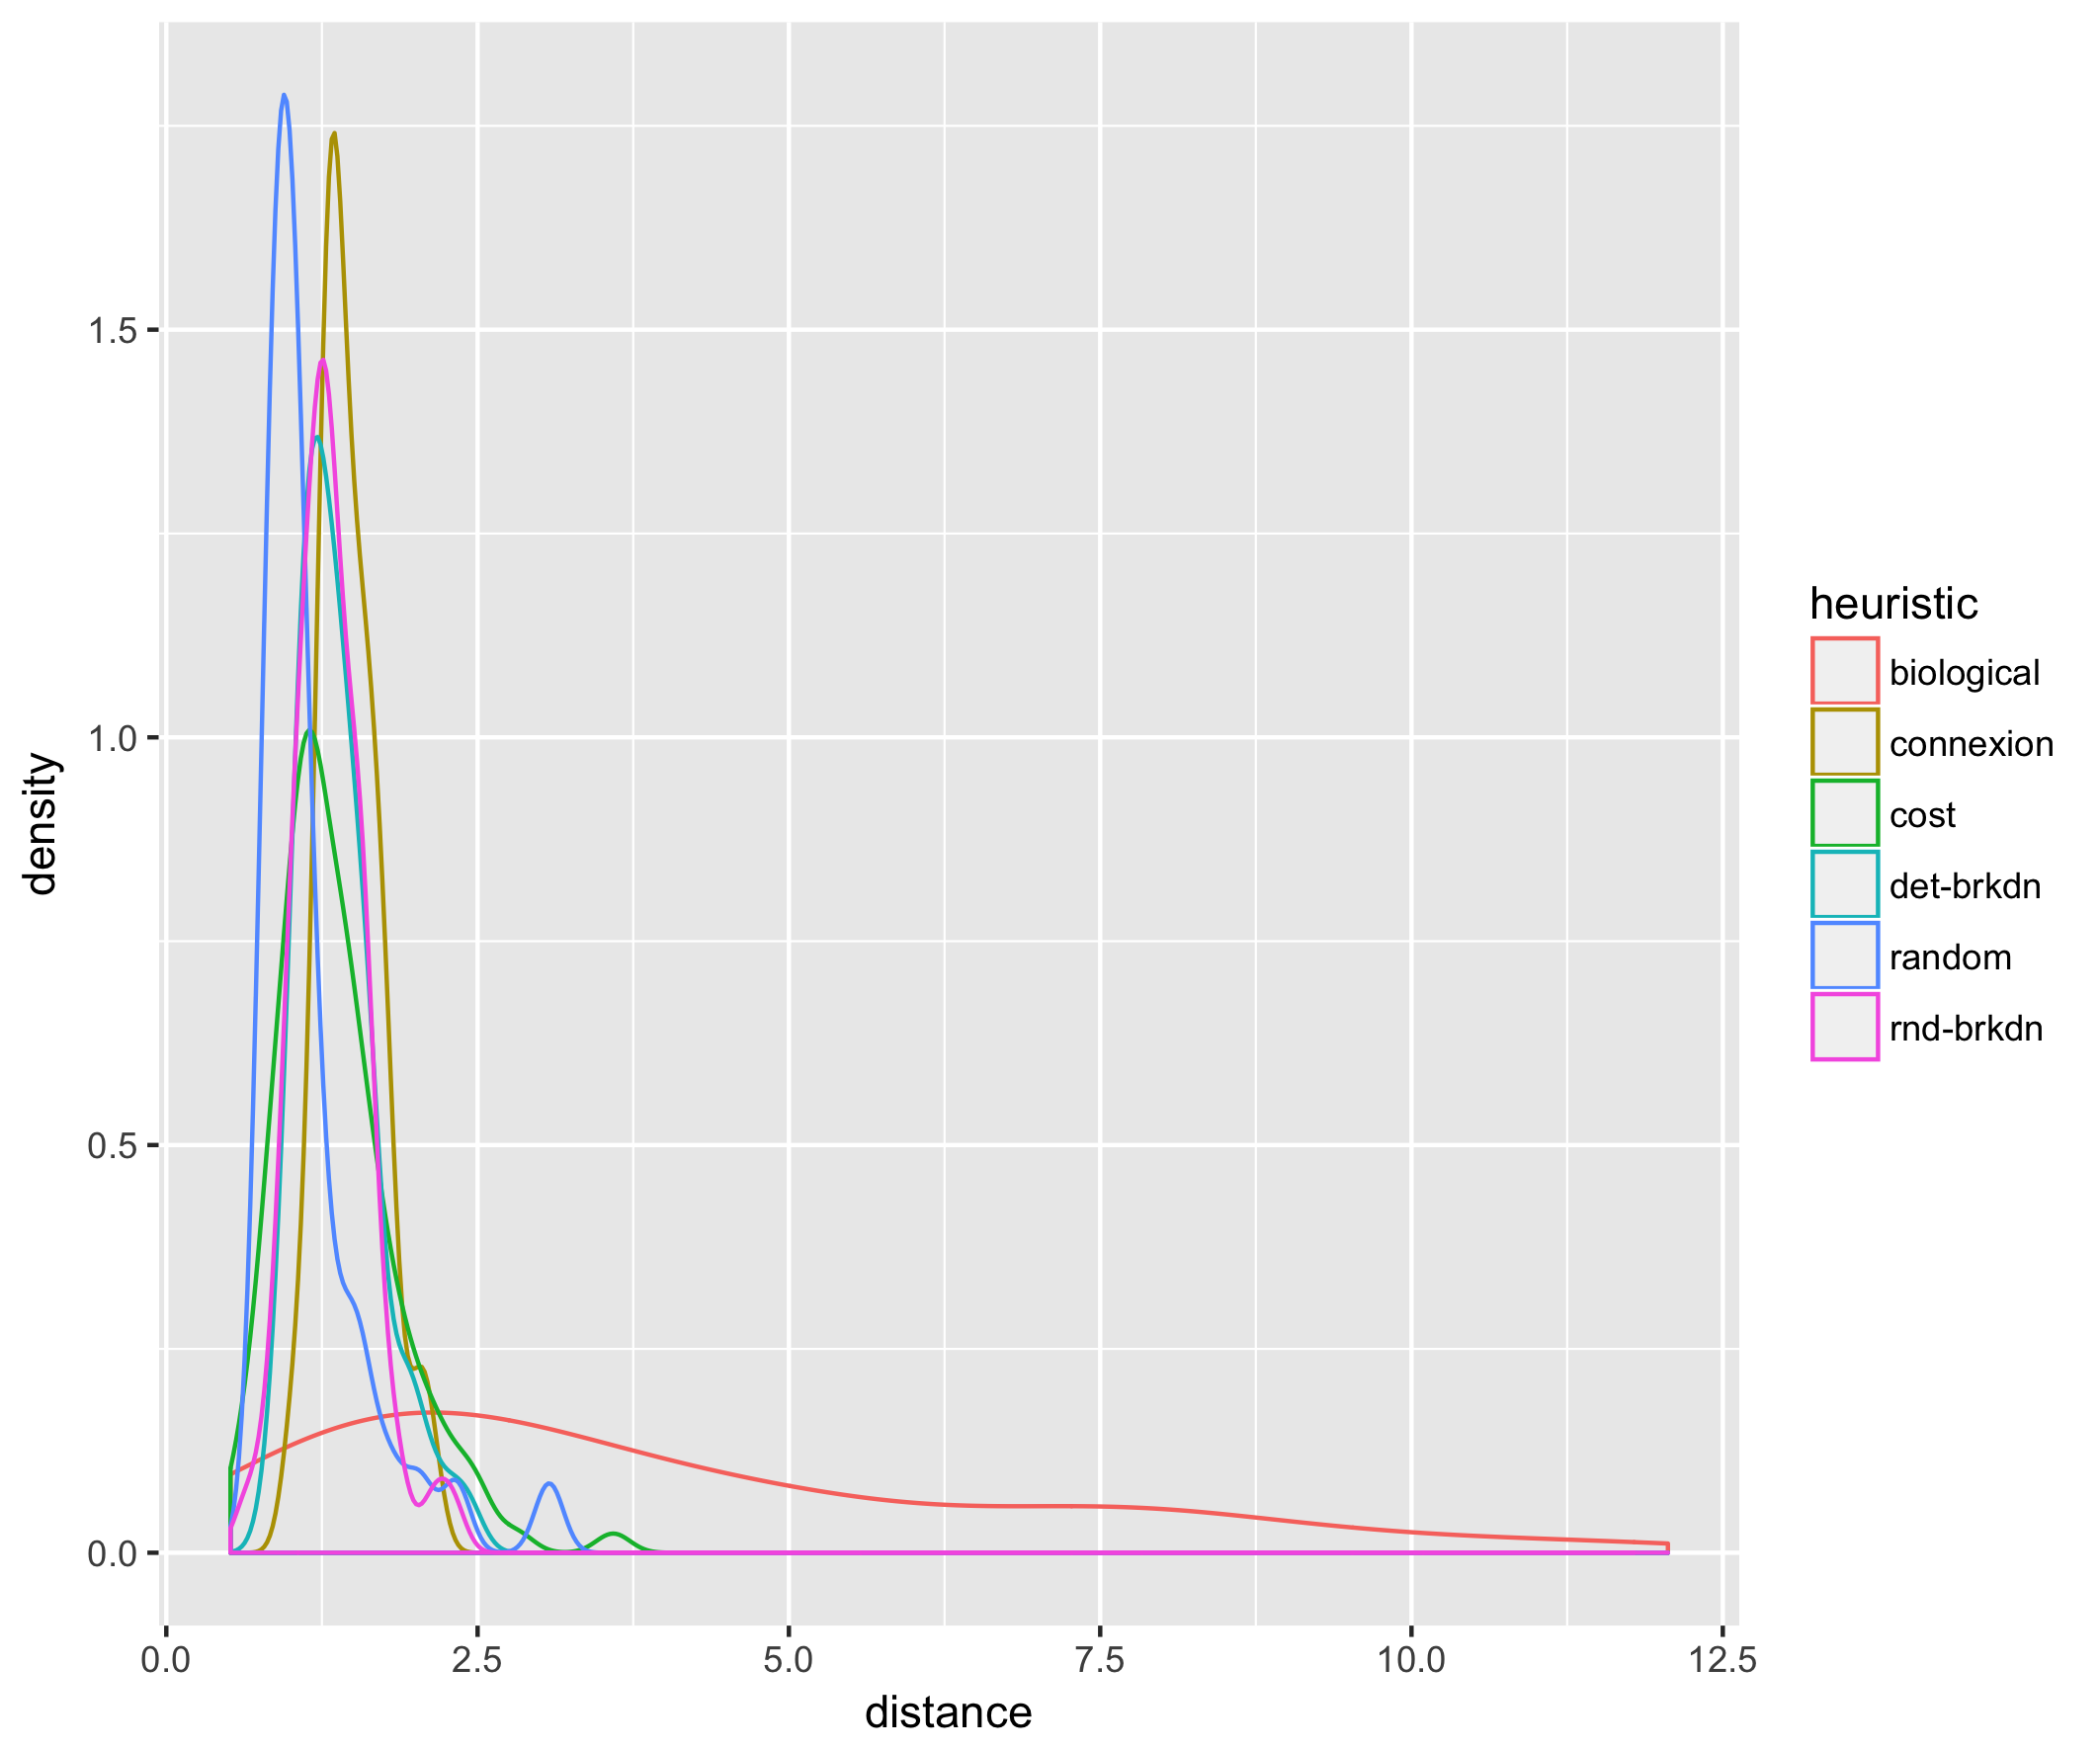
\includegraphics[width=\textwidth]{figures/coevol_corrs-distrib_rhoasize4}
%
%\end{columns}
%
%\footnotesize\textit{(Left) Full indicator space; (Middle) Morphological and Topology, by network heuristic; (Right) Distance distribution for cumulated distance for indicators and correlations.}
%
%}
%
%
%\sframe{Results : Causality Regimes}{
%
%\textit{Unsupervised learning on lagged correlations between local variables unveils a diversity of causality regimes}
%
%$\rightarrow$ Link between \emph{co-evolution regime} and morphogenetic properties of the urban system
%
%% comment Arnaud : le genre d’affirmation qu’il faut réussir à exprimer également du point de vue de l’objet étudié : qu’est-ce que ça veut dire pour la morphogénèse urbaine ?
%
%\medskip
%
%\centering
%
%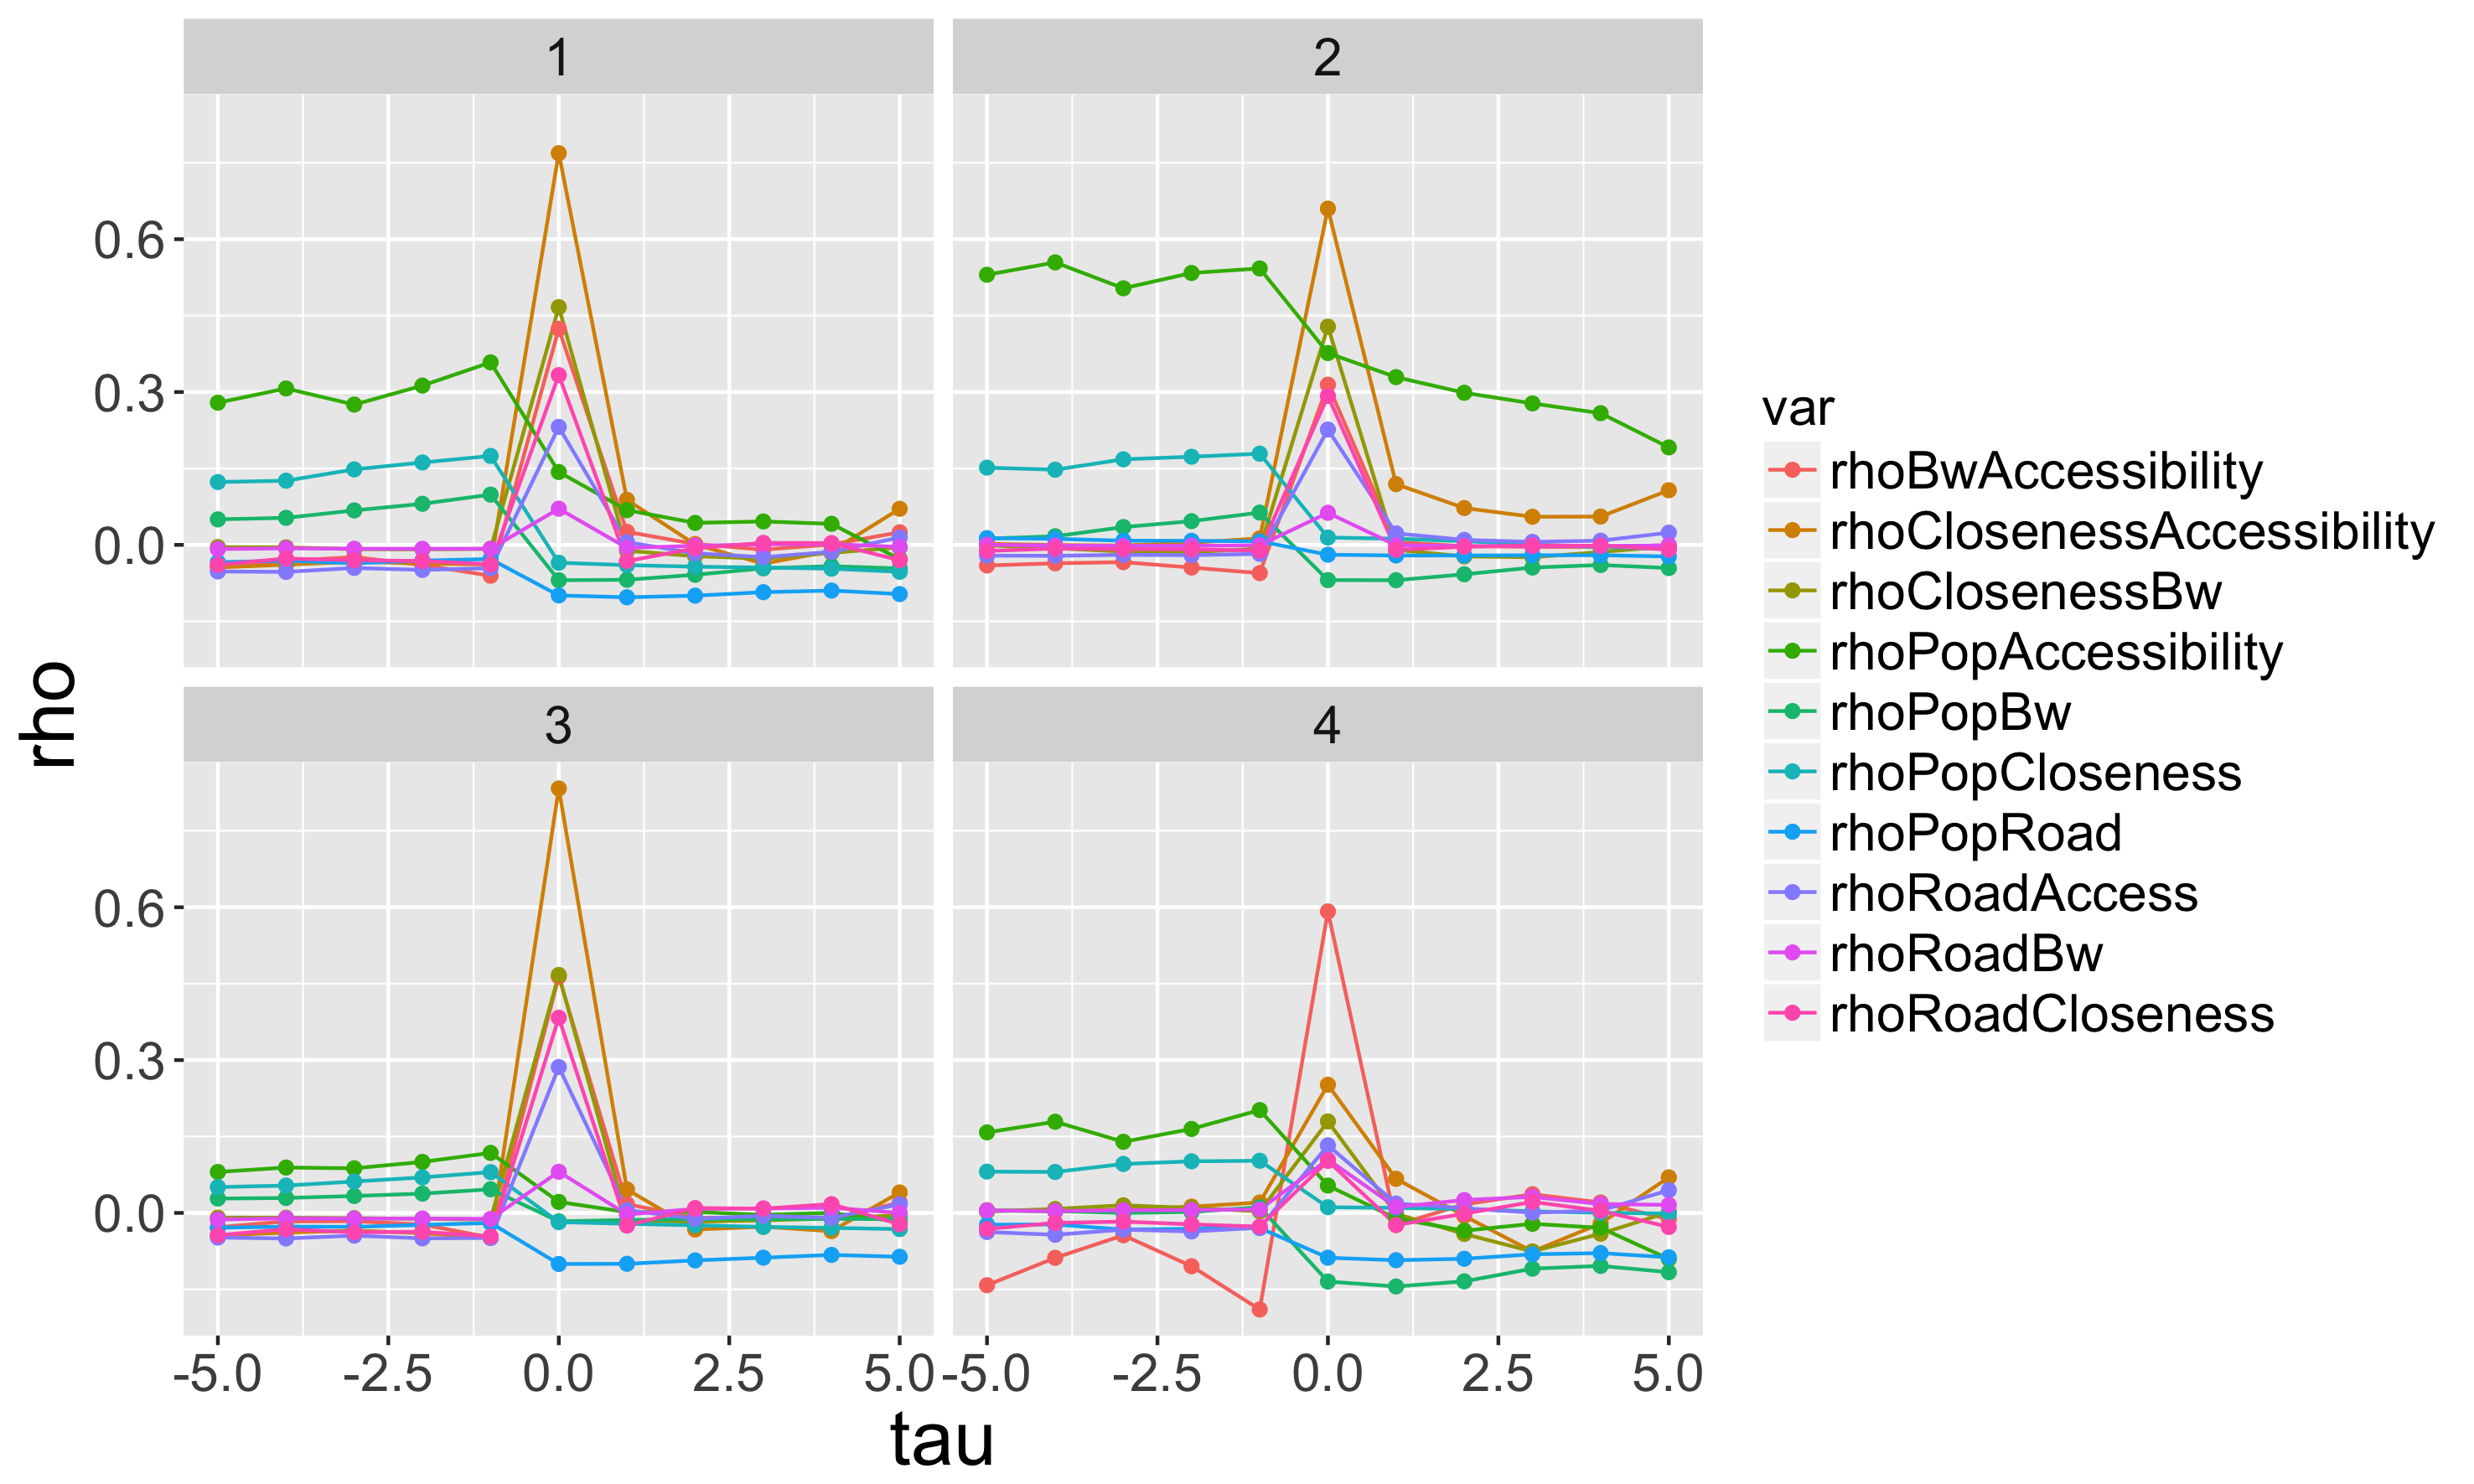
\includegraphics[width=0.52\textwidth,height=0.55\textheight]{figures/coevol_centertrajs}
%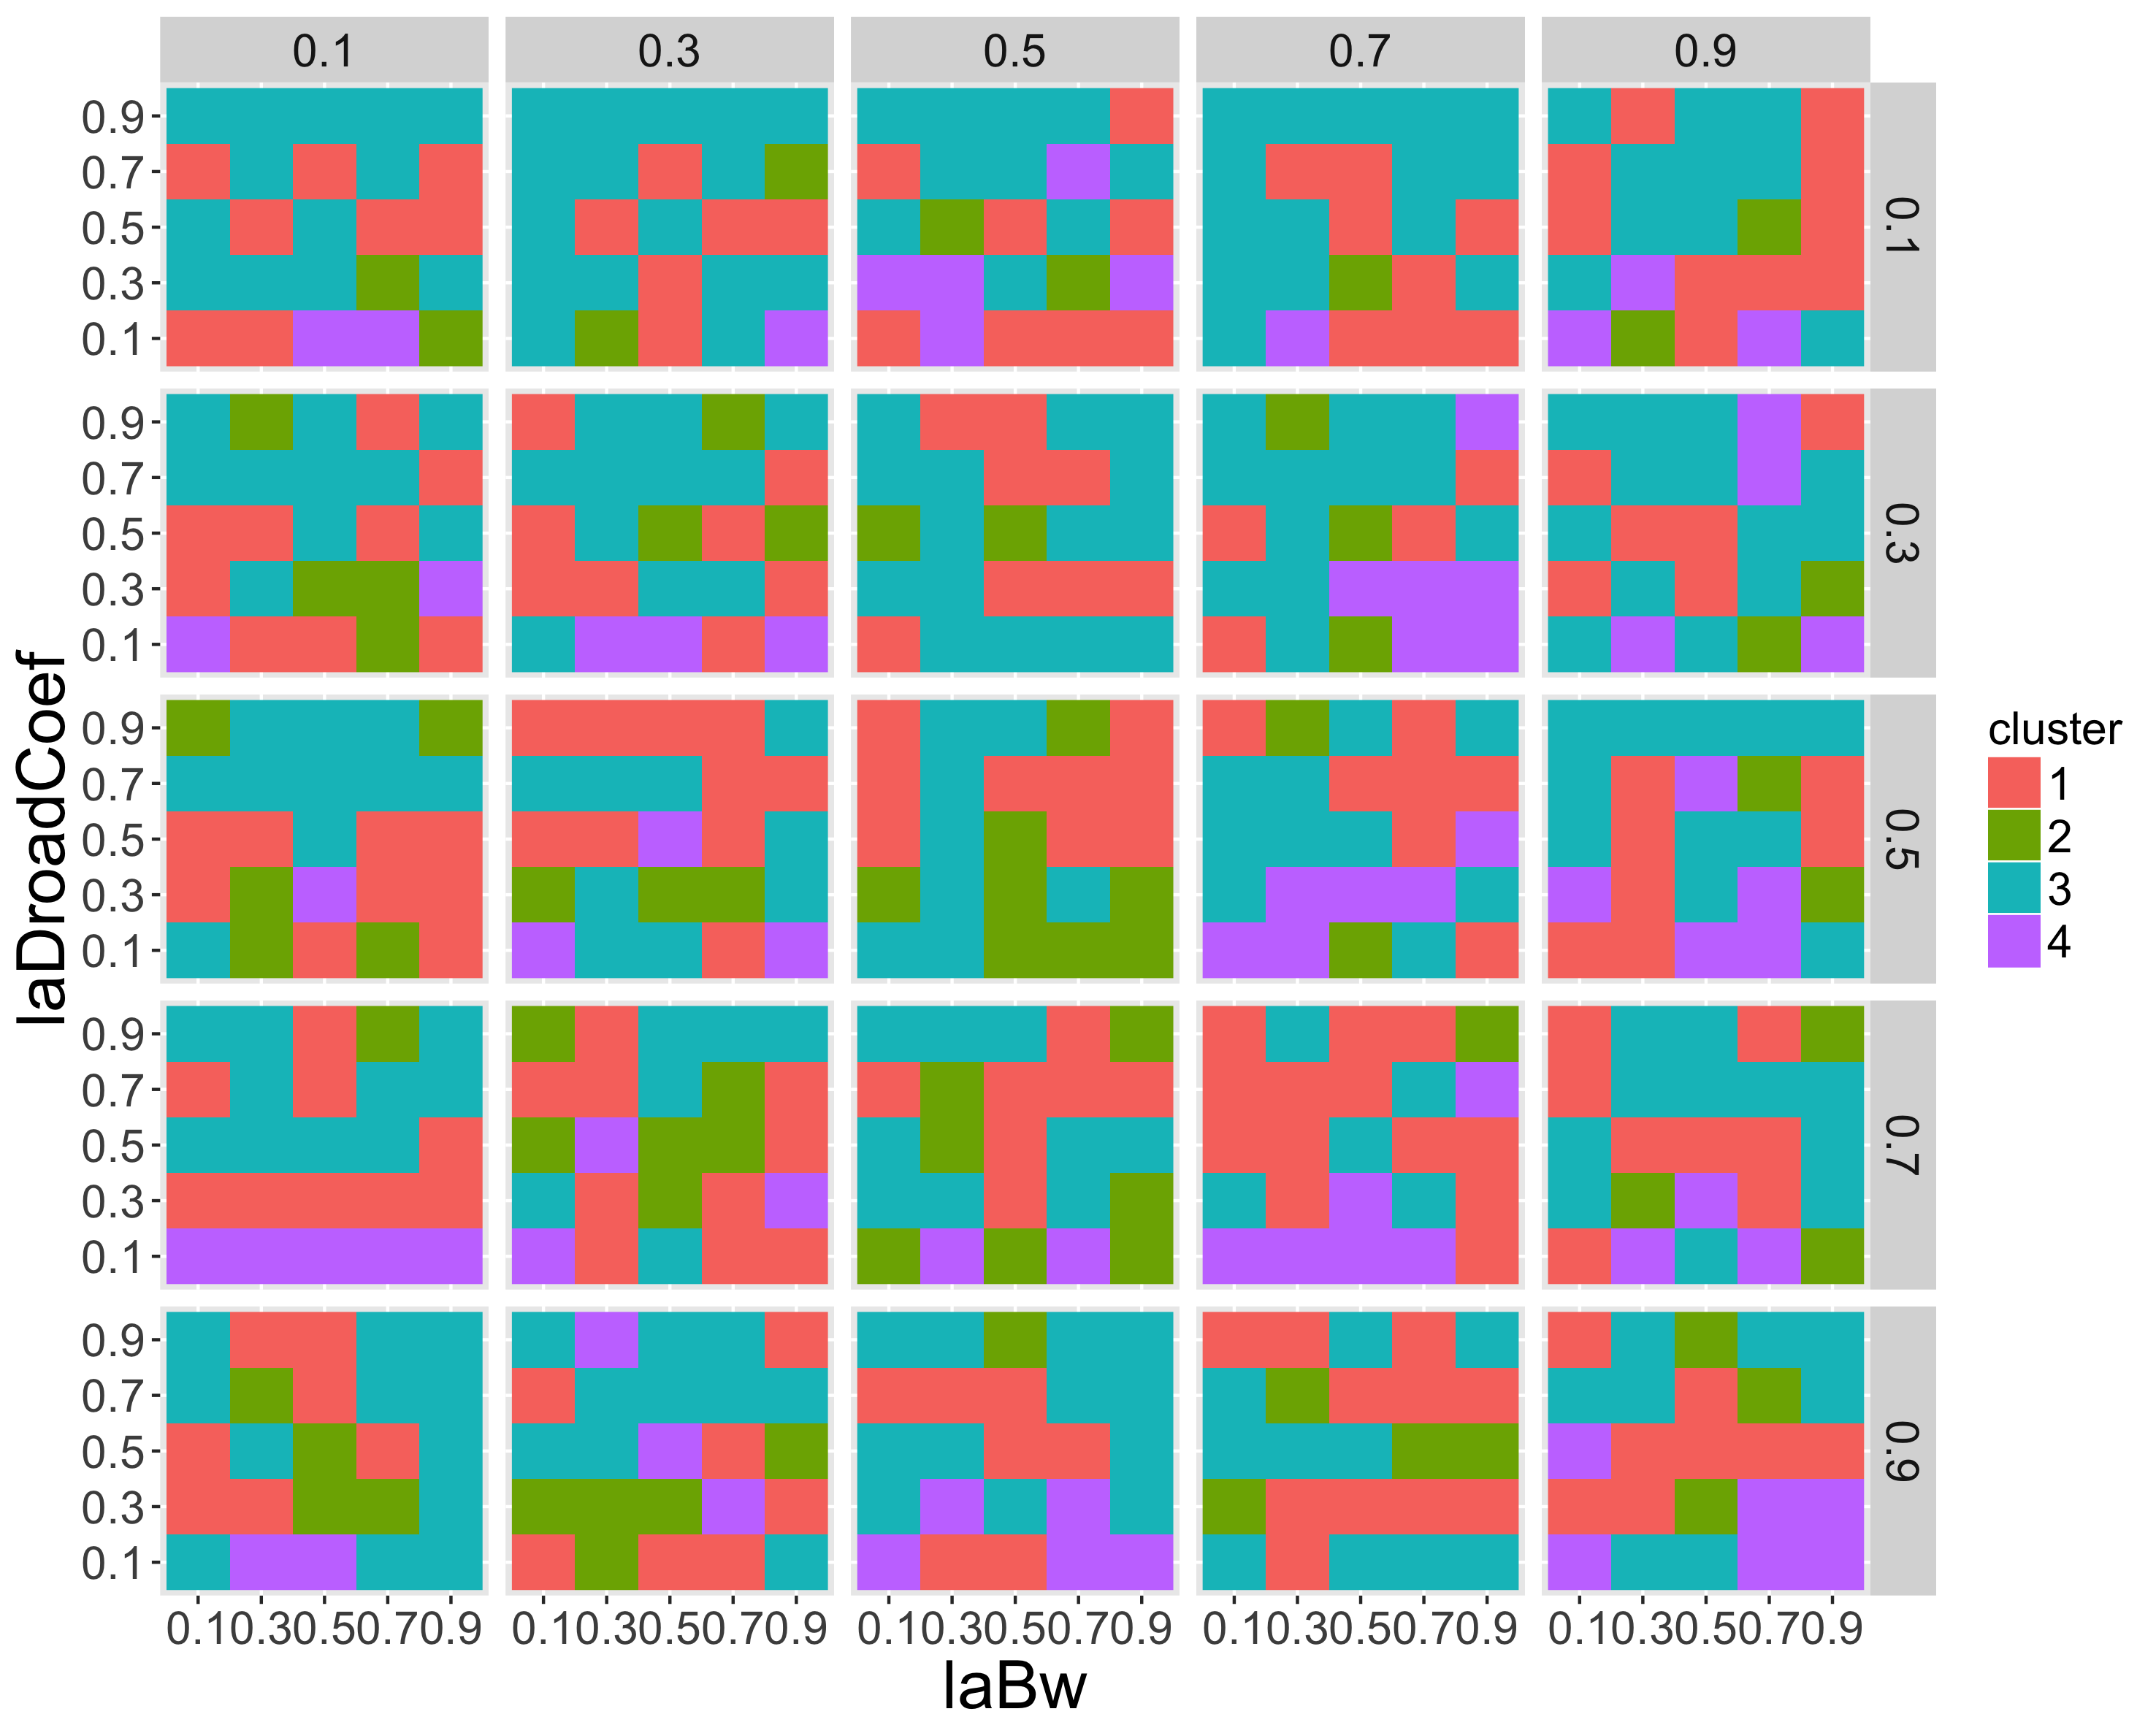
\includegraphics[width=0.4\textwidth,height=0.55\textheight]{figures/coevol_cluster-params}
%
%\footnotesize\textit{(Left) Lagged correlation profiles of cluster centers; (Right) Distribution of regimes across parameter space}
%
%}
%
%
%
%\sframe{Discussion}{
%
%\justify
%
%\vspace{-1cm}
%
%\textbf{Implications}
%
%$\rightarrow$ This rather simple model reproduces most of existing urban forms in Europe for both population distribution and road network : which intrinsic dimension to the urban system and its morphological aspect ?
%
%$\rightarrow$ Ability to reproduce static correlations and a variety of dynamical lagged correlation regimes suggests that the model captures some of the processes of co-evolution
%
%% implications for morphogenesis ?
%
%\bigskip
%
%\textbf{Developments}
%
%
%$\rightarrow$ Towards a dynamical calibration ? Need of dynamical data
%
%$\rightarrow$ Investigate the link between spatial non-stationarity and non-ergodicity through simulation by the model
%
%$\rightarrow$ Compare network generation in a ``fair'' way (correcting for additional parameters, open question for models of simulation)
%
%
%}
%
%
%
%\sframe{Conclusion}{
%
%
%\justify
%
%$\rightarrow$ A novel model of urban morphogenesis at the mesoscopic scale systematically explored : \textbf{need for more coupling and comparison of models.}
%
%\medskip
%
%$\rightarrow$ At the macro scale of the system of cities ? \textbf{Need for multi-scale models.}
%
%\medskip
%
%$\rightarrow$ With more refined urban characteristics and other dimensions ? \textbf{Need for more interdisciplinarity.}
%
%\bigskip
%\bigskip
%\bigskip
%
%\footnotesize{ - Code, data and results available at\\ \texttt{https://github.com/JusteRaimbault/CityNetwork}\\
%- Paper on arXiv at \texttt{https://arxiv.org/abs/1708.06743}\\
%- Acknowledgments : We thank the \textit{European Grid Infrastructure} and its \textit{National Grid Initiatives} (\textit{France-Grilles} in particular) to give the technical support and the infrastructure.
%
%}
%
%}
%
%
%
%
%
%
%\sframe{Reserve slides}{
%
%\centering
%
%\Large
%
%\textbf{Reserve Slides}
%
%}
%
%
%
%
%%%%%%%%%%%%%%%%%%
%%\section*{Morphogenesis}
%
%
%
%\sframe{Morphogenesis Overview}{
%% other numerous examples of fields/case of application
%
%\cite{bourgine2010morphogenesis} : interdisciplinary workshop on morphogenesis
%
%\bigskip
%
%$\rightarrow$\textit{To what extent the notion is indeed transdisciplinary, i.e. are there common definitions across disciplines ? What are the concepts shared or the divergence ?}
%
%
%\begin{itemize}
%\item \textbf{Biology}
%\begin{itemize}
%\item External phenotype morphogenesis (ant colony)~\cite{minter2012morphogenesis} \item Symbiosis of species~\cite{chapman1998morphogenesis}
%\item Botany~\cite{lord1981cleistogamy}
%\end{itemize}
%\item \textbf{Social Sciences} : Archeology~\cite{renfrew1978trajectory}
%\item \textbf{Epistemology} : \cite{gilbert2003morphogenesis}
%\item \textbf{Artificial Intelligence} : From self-assembly to Morphogenetic Engineering~\cite{doursat2013review}. Synthetic Biology ?
%\item \textbf{Geomorphology} : dunes formation~\cite{douady2011dunes}
%\item \textbf{Physics} : Arbotrons playing Tetris ?
%\item etc\ldots
%\end{itemize}
%
%
%
%
%}
%
%
%
%\sframe{Morphogenesis concepts}{
%
%\begin{itemize}
%\item \justify \textbf{Morphogenesis and Self-Organisation} : when does a system exhibit an architecture ? Insights from Morphogenetic Engineering
%\cite{doursat2013review}. Architecture : the relation between the form and the function ?
%\medskip
%\end{itemize}
%\begin{itemize}
%\item \justify\textbf{Scales, Units and Boundaries} From local interactions to global information flow (Holland's \emph{signal and boundaries}~\cite{holland2012signals}: morphogenesis as the development of Complex Adaptive Systems ?)
%\medskip
%\end{itemize}
%\begin{itemize}
%\item \justify \textbf{Symmetry and Bifurcations} : on quantitative becoming qualitative. Ren{\'e} Thom's \emph{theory of catastrophes}~\cite{thom1974stabilite}
%\medskip
%\end{itemize}
%\begin{itemize}
%\item \justify \textbf{Life and Death} : link with autopoiesis and cognition\\
%\cite{bourgine2004autopoiesis} ; co-evolution of subsystems as an alternative definition ? In psychology, attractors of the mind.
%\end{itemize}
%
%
%}
%
%
%\sframe{Catastrophe Theory}{
%
%% brief rapide sur theorie des catastrophes
%
%A system is viewed as its internal state $X_w$, where $w\in W$ is a control parameter.
%
%\bigskip
%
%Catastrophe set $K \subset W$ is where the system endures phase transition.
%
%\bigskip
%
%Thom classified possible topologies for $K$ depending on the dimension of $W$.
%
%}
%
%
%
%\sframe{Modeling Urban Morphogenesis}{
%
%\justify
%
%\cite{makse1998modeling} correlated growth; 
%
%\cite{10.1371/journal.pone.0133780} multi-scale migration and percolation; 
%
%\cite{bonin2012modele} qualitative differentiation of urban function; 
%
%\cite{achibet2014model} procedural model at the micro-scale 
%
%}
%
%
%
%
%%%%%%%%%%%%%%%%%%
%%\section*{Density Morphogenesis}
%
%
%
%
%
%\sframe{Model classification : PDE}{
%
%% derived PDE
%
%The one-dimensional model verifies the PDE :
%
%\begin{equation}\label{eq:pde}
%\begin{split}
%\delta t \cdot \frac{\partial p}{\partial t} = \frac{N_G \cdot p^{\alpha}}{P_{\alpha}(t)} + \frac{\alpha \beta (\alpha - 1) \delta x^2}{2}\cdot \frac{N_G \cdot p^{\alpha-2}}{P_{\alpha}(t)} \cdot \left(\frac{\partial p}{\partial x}\right)^2\\
%+ \frac{\beta \delta x^2}{2} \cdot \frac{\partial^2 p}{\partial x^2} \cdot\left[ 1 + \alpha \frac{N_G p^{\alpha - 1}}{P_{\alpha(t)}} \right]
%\end{split}
%\end{equation}
%
%}
%
%
%\sframe{Stationary behavior of 1D model}{
%\centering
%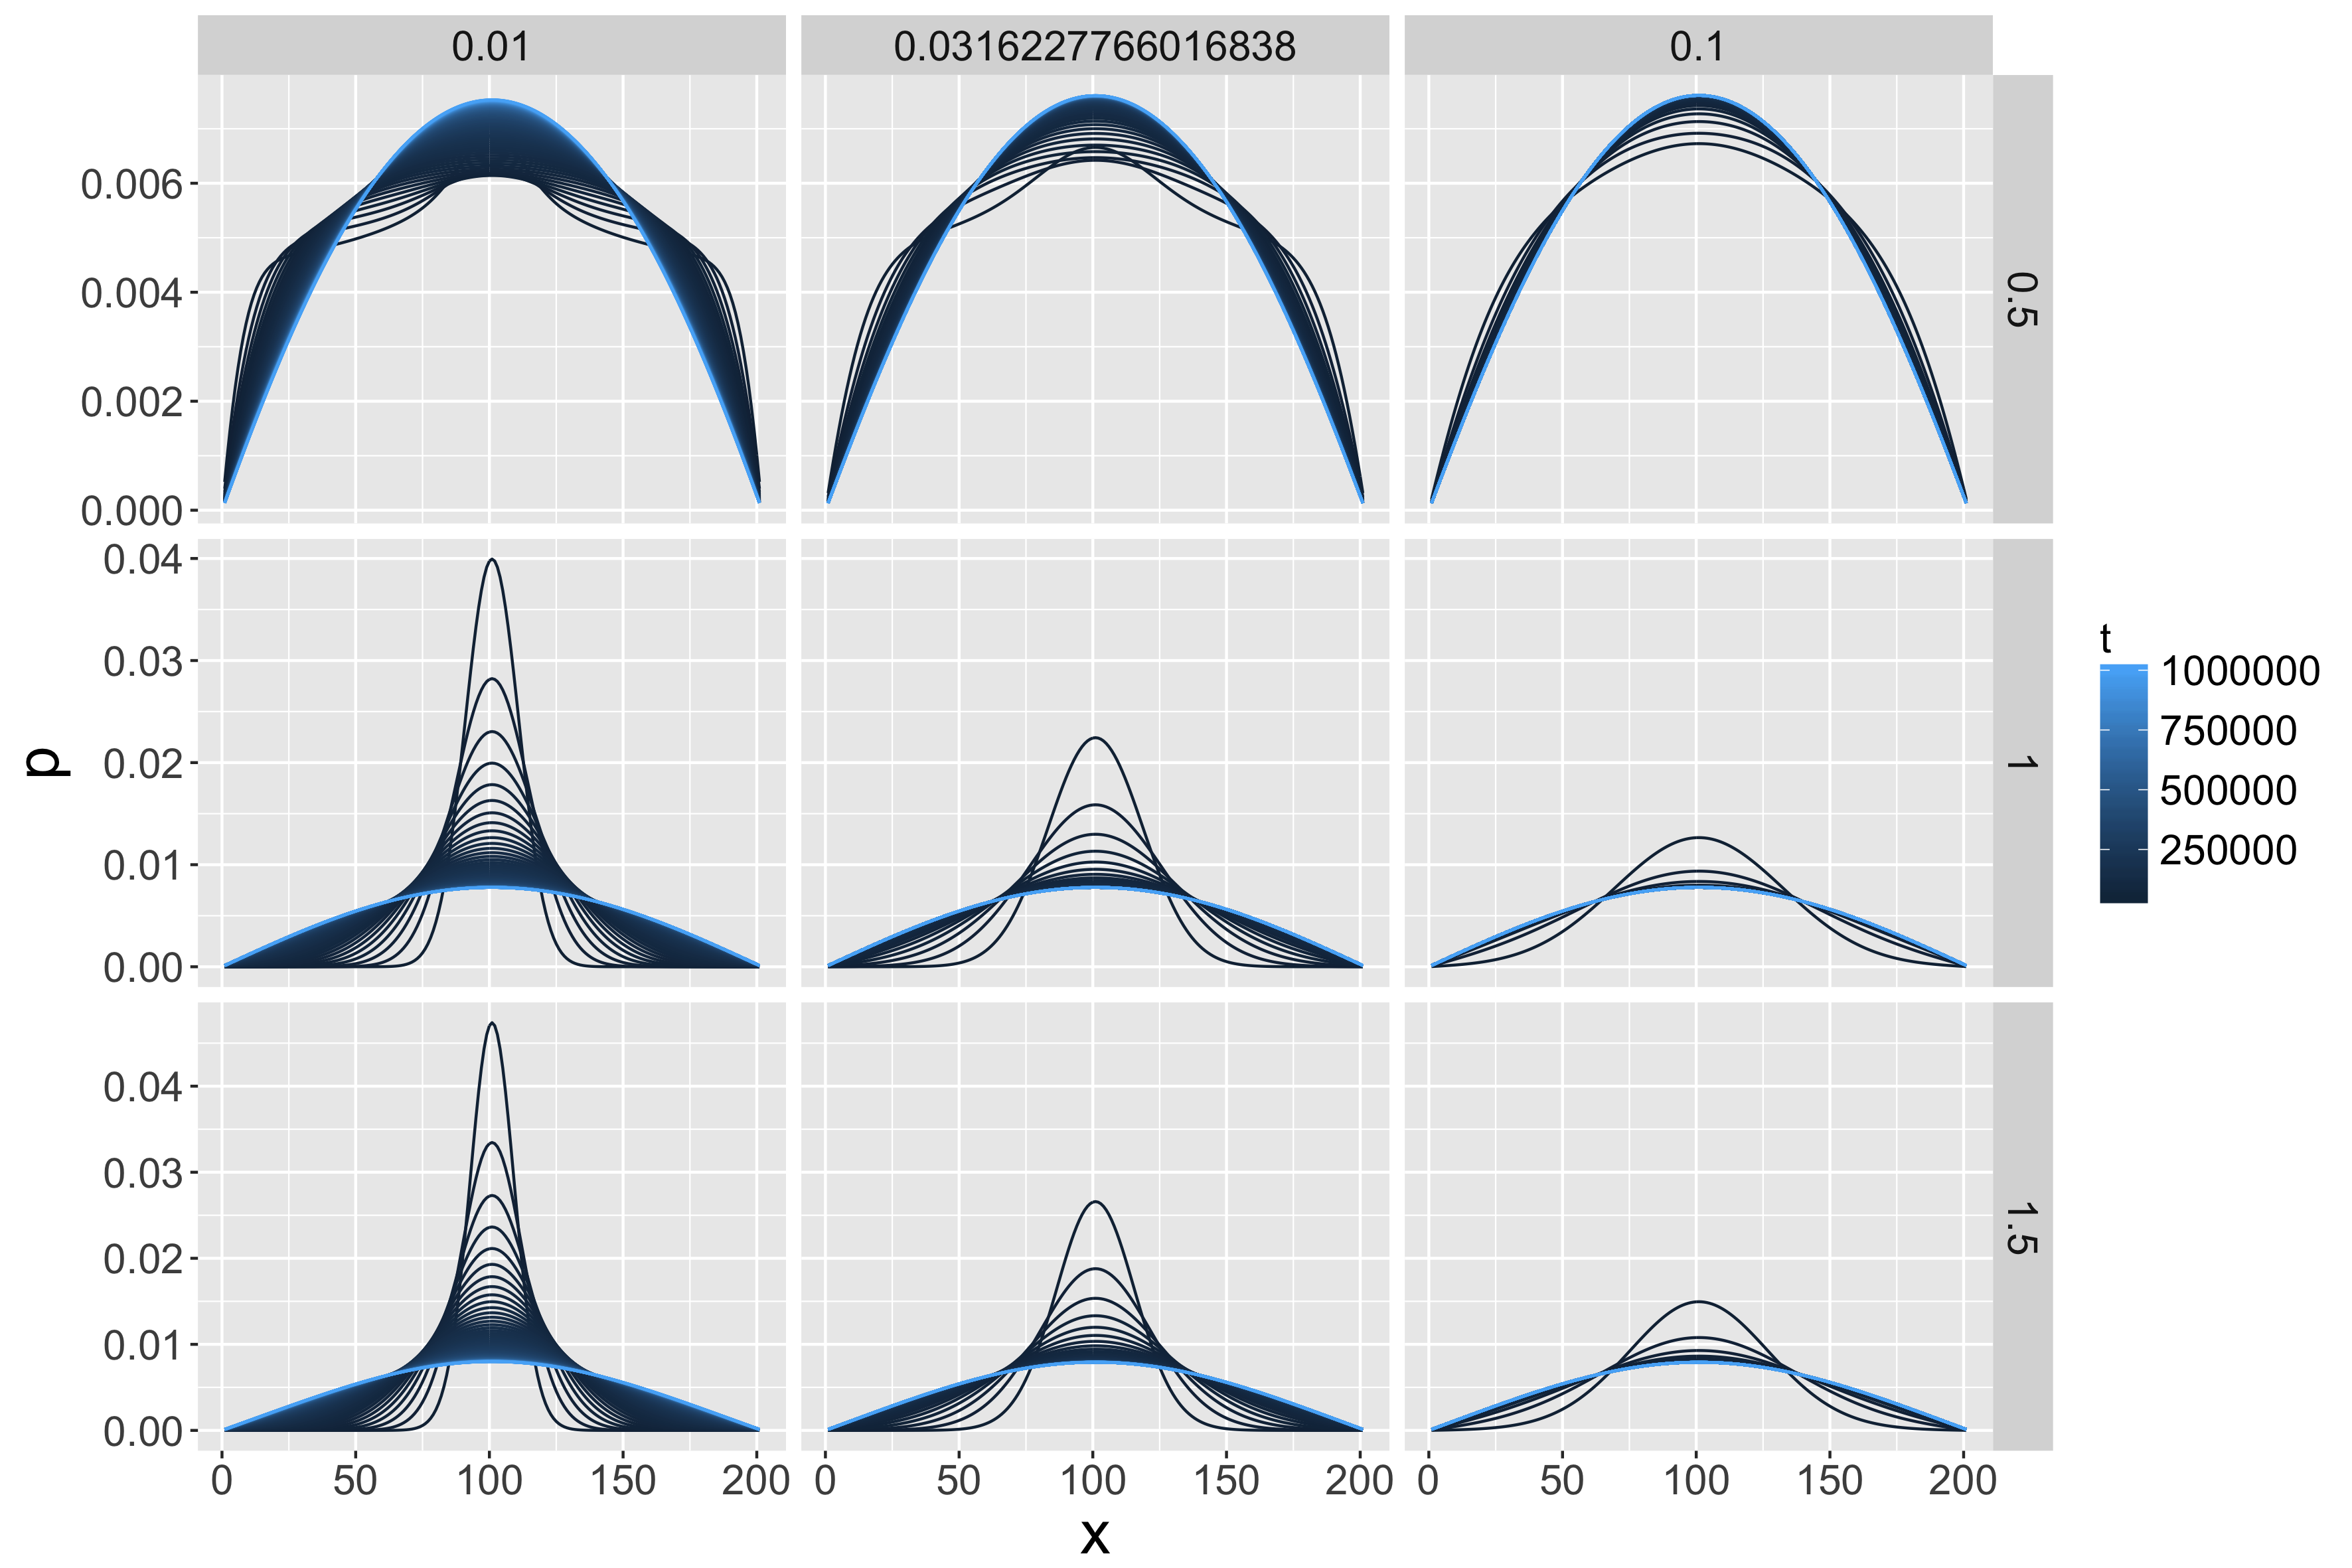
\includegraphics[width=\textwidth]{figures/density_stationary}
%}
%
%\sframe{Stationary behavior of 1D model}{
%\centering
%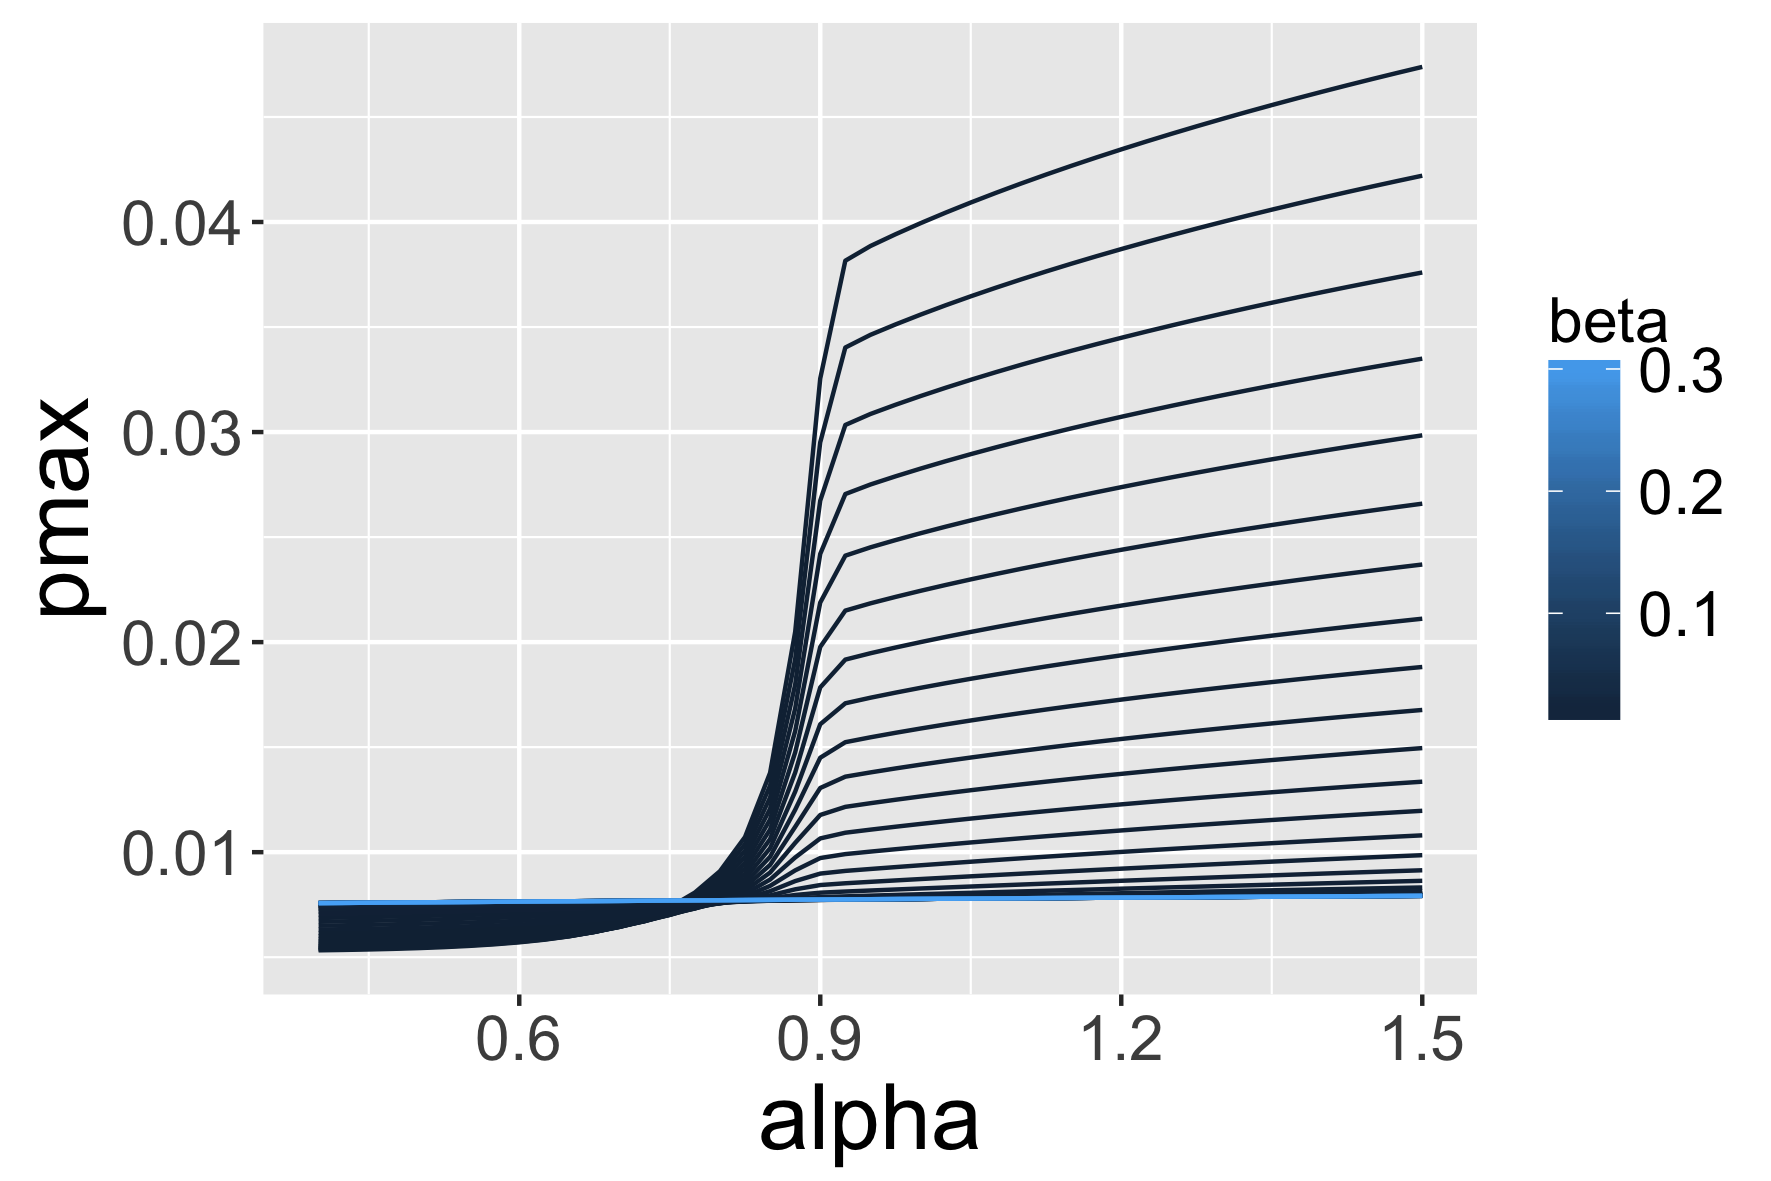
\includegraphics[width=0.48\textwidth]{figures/density_pmax_alpha}
%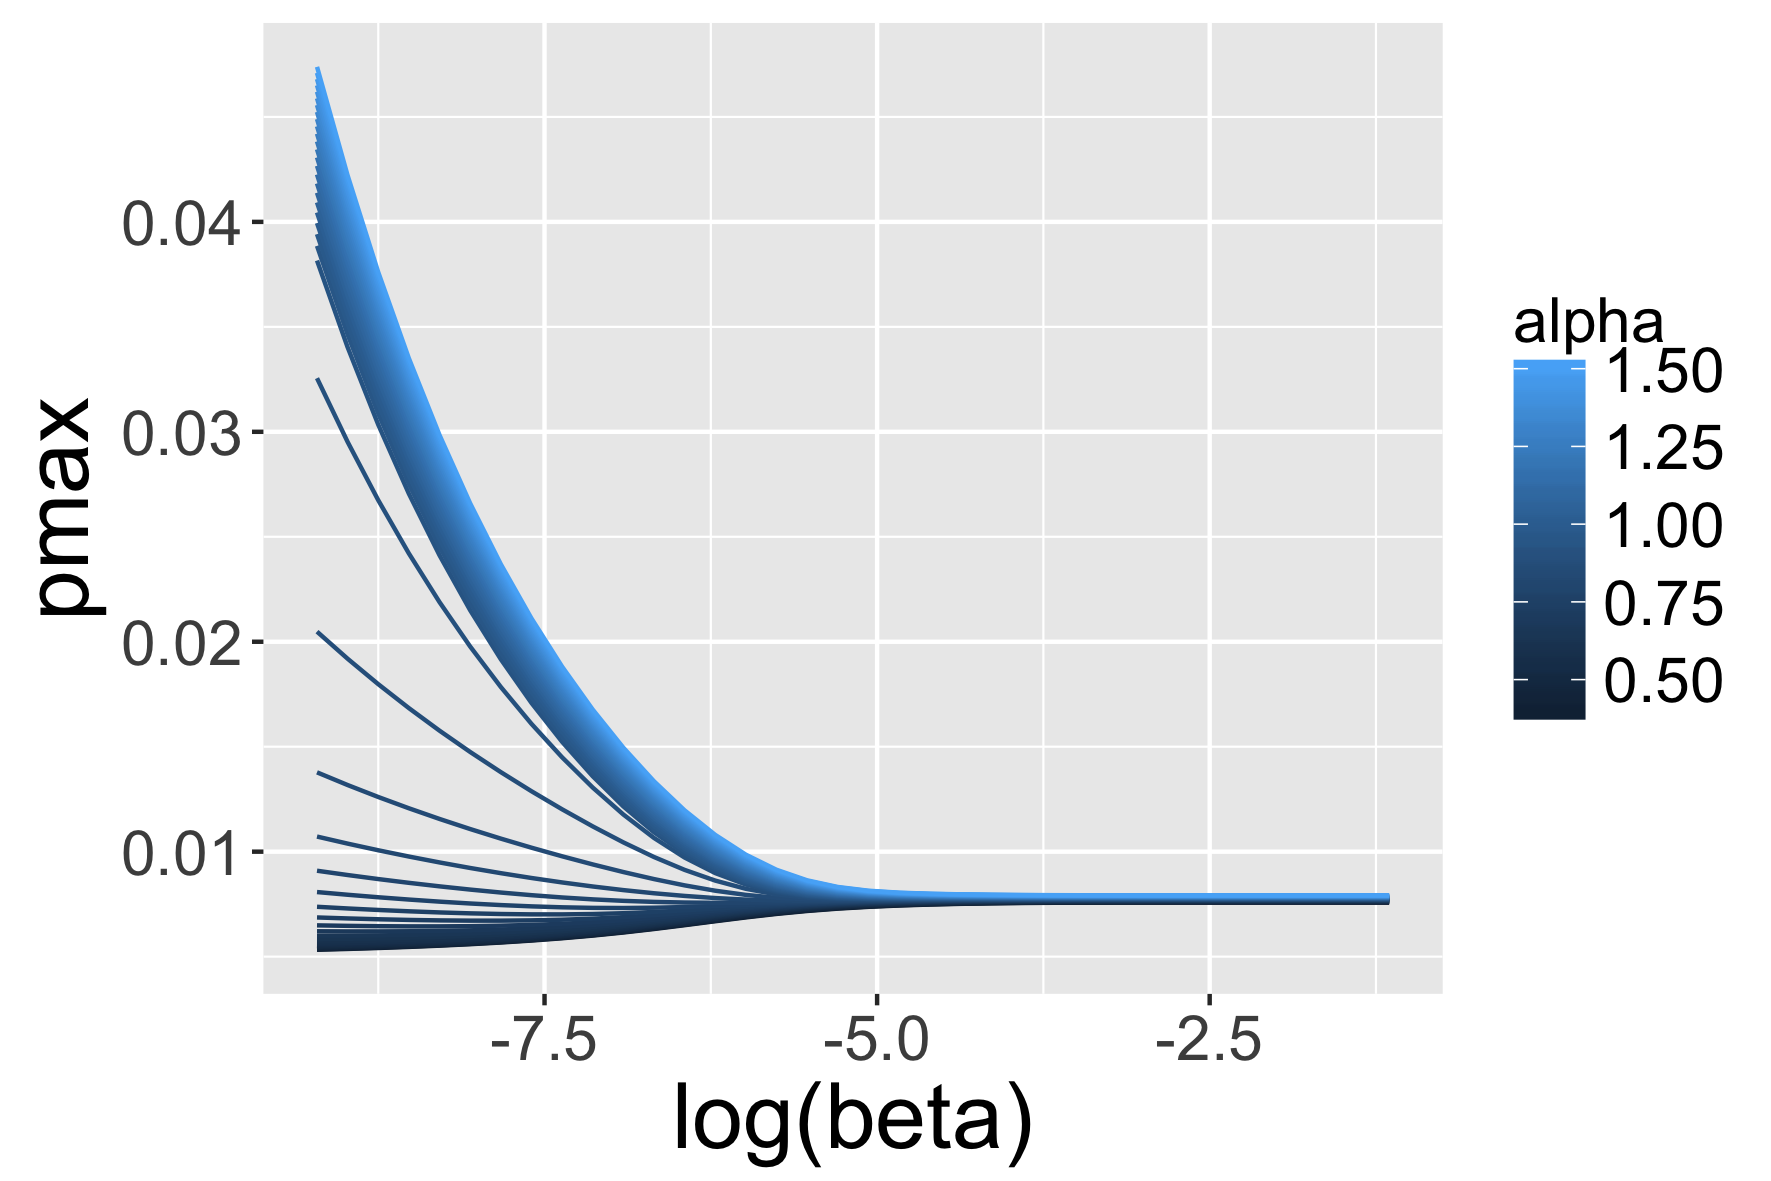
\includegraphics[width=0.48\textwidth]{figures/density_pmax_logbeta}
%
%}
%
%
%
%\sframe{Morphological indicators}{
%
%\begin{enumerate}
%\item Rank-size slope $\gamma$, given by $\ln \left( P_{\tilde{i}}/P_0\right) \sim k + \gamma\cdot \ln \left(\tilde{i}/i_0\right)$ where $\tilde{i}$ are the indexes of the distribution sorted in decreasing order.
%\item Entropy of the distribution:
%\begin{equation}
%\mathcal{E} = \sum_{i=1}^{M}\frac{P_i}{P}\cdot \ln{\frac{P_i}{P}}
%\end{equation}
%$\mathcal{E}=0$ means that all the population is in one cell whereas $\mathcal{E}=0$ means that the population is uniformly distributed.
%\item Spatial-autocorrelation given by Moran index, with simple spatial weights given by $w_{ij} = 1/d_{ij}$
%\[
%I = M \cdot \frac{\sum_{i\neq j} w_{ij} \left(P_i - \bar{P}\right)\cdot\left(P_j - \bar{P}\right)}{\sum_{i\neq j} w_{ij} \sum_{i}{\left( P_i - \bar{P}\right)}^2}
%\]
%\item Mean distance between individuals
%\[
%\bar{d} = \frac{1}{d_M}\cdot \sum_{i<j} \frac{P_i P_j}{P^2} \cdot d_{ij}
%\]
%where $d_M$ is a normalisation constant
%\end{enumerate}
%
%
%
%}
%
%
%\sframe{Model behavior : Convergence}{
%
%Large number of repetitions show good convergence properties
%
%% hist examples
%
%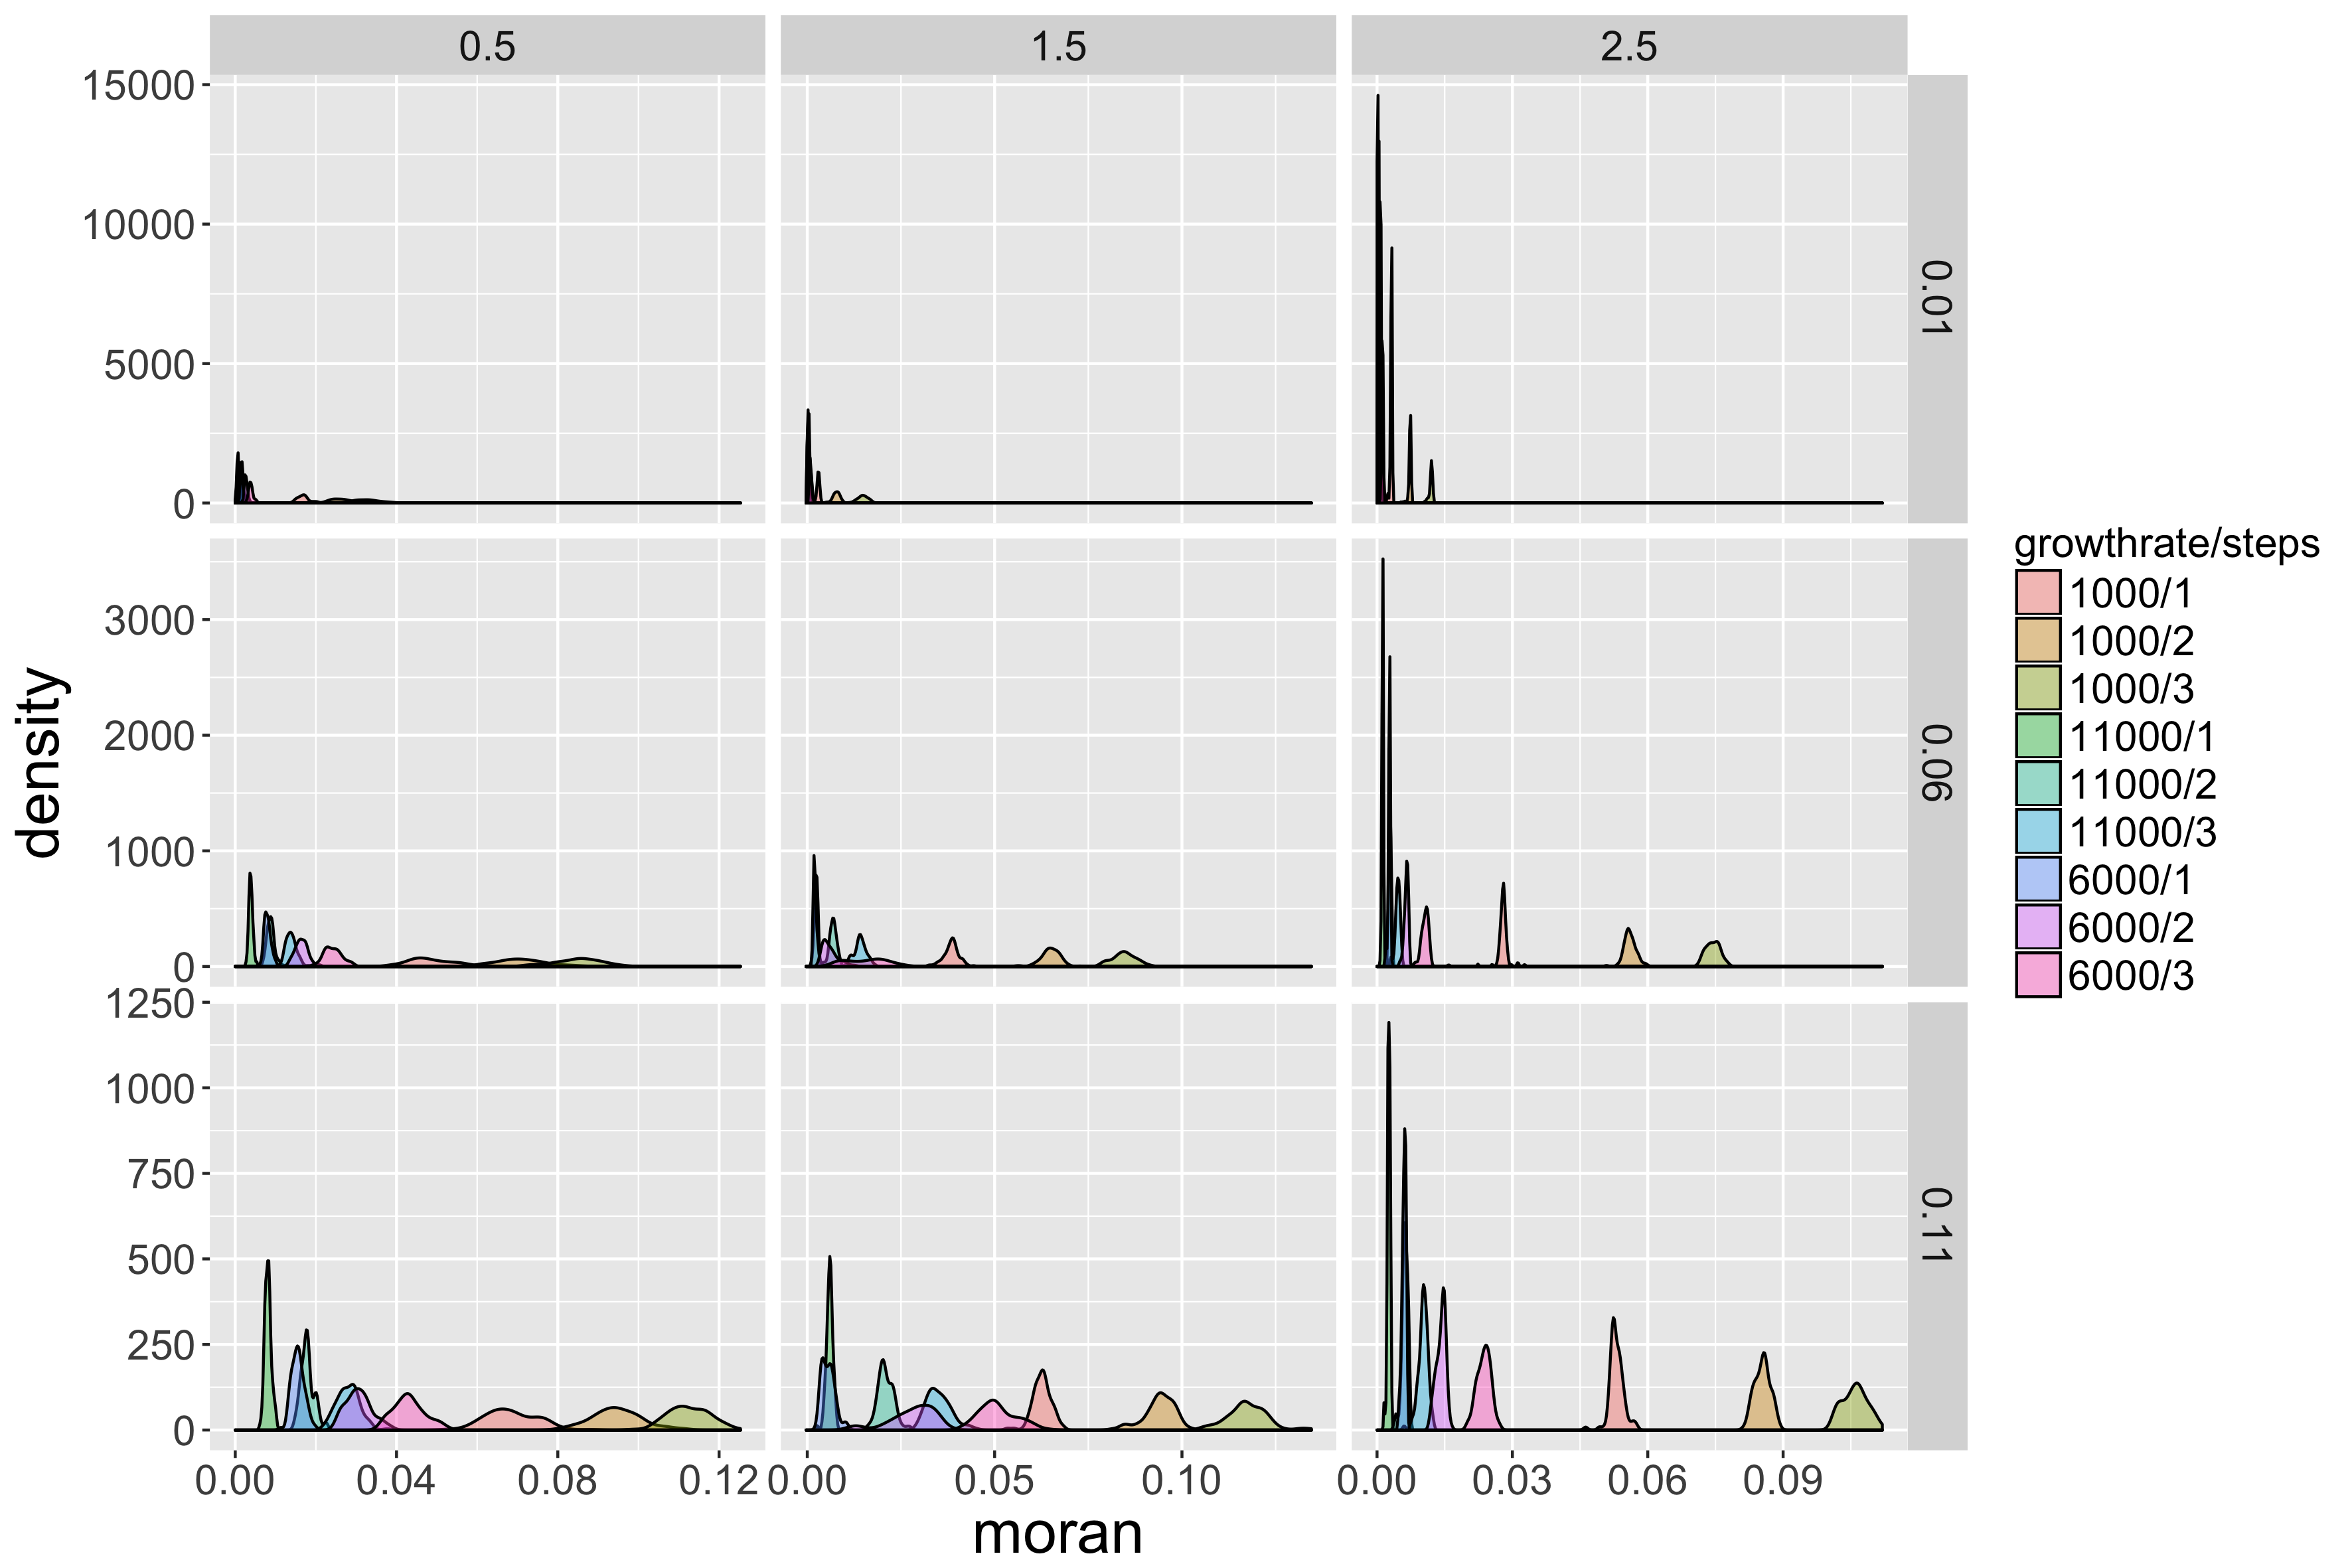
\includegraphics[width=0.5\textwidth]{figures/density_hist_moran}
%\includegraphics[width=0.5\textwidth]{figures/density_hist_slope}
%
%}
%
%
%\sframe{Model behavior}{
%
%
%\includegraphics[width=0.5\textwidth]{figures/density_pc_colalpha}
%\includegraphics[width=0.5\textwidth]{figures/density_pc_colbeta}
%
%}
%
%
%\sframe{Empirical indicators computation}{
%
%$\rightarrow$ Eurostat population density raster (100m, simplified at 500m resolution)
%
%\medskip
%
%$\rightarrow$ Overlapping (10km offset) squares of 50km side : equivalent to smoothing, removes window shape effect. Not very sensitive to window size (tested with 30km and 100km)
%
%\medskip
%
%$\rightarrow$ Indicators computed using Fast Fourier Transform Convolution
%
%\medskip
%
%$\rightarrow$ Classification using repeated k-means ; number of clusters taken at transition in clustering coefficient.
%
%}
%
%\sframe{Model calibration: all indicators}{
%
%\centering
%\includegraphics[width=0.8\textwidth]{figures/density_scatter}
%
%}
%
%
%
%
%%%%%%%%%%%%%%%%%%
%%\section*{Co-evolution Morphogenesis}
%
%
%
%
%\sframe{Defining co-evolution}{
%
%
%\justify
%
%No clear definition of co-evolution in the literature : \cite{bretagnolle:tel-00459720} distinguishes ``reciprocal adaptation'' where a sense of causality can clearly be identified, from co-evolutive regimes 
%
%
%\bigskip
%\bigskip
%
%Identification of multiple causality regimes in a simple strongly coupled growth model $\rightarrow$ to be put in perspective with a theoretical definition of co-evolution based on the conjunction of Morphogenesis and the Evolutive Urban Theory, summarised by~\cite{raimbault2017co}
%
%}
%
%
%\sframe{Modeling Co-evolution}{
%
%\justify
%
%\cite{baptistemodeling} system dynamics with evolving capacities
% 
%\cite{wu2017city} population diffusion and network growth
%
%\cite{blumenfeld2010network} and \cite{schmitt2014modelisation} : random potential breakdown for network growth.
%
%\cite{barthelemy2009co} geometrical network growth model making network topology co-evolve with vertex density
%
%}
%
%
%\sframe{Empirical Data : network indicators}{
%
%\centering
%
%\includegraphics[width=0.53\textwidth]{figures/coevol_FR_indics_network_selected_2_discrquantiles}
%
%}
%
%\sframe{Empirical Data : correlations}{
%
%\centering
%\includegraphics[width=0.7\textwidth]{figures/coevol_FR_corr_PCA_rhoasize12}
%
%}
%
%
%
%\sframe{Network Indicators}{
%
%Network Topology measured by:
%
%\begin{itemize}
%	\item Betweenness and Closeness centralities: average and hierarchy
%	\item Accessibility (weighted closeness)
%	\item Efficiency (network pace relative to euclidian distance)
%	\item Mean path length, diameter
%\end{itemize}
%
%}
%
%
%
%
%\sframe{Model specification}{
%
%\footnotesize
%
%Patch utility given by $U_i = \sum_k w_k \cdot \tilde{x}_k$ with $\tilde{x}_k$ normalized local variables among population, betweenness and closeness centrality, distance to roads, accessibility ; aggregation done with probability $\left(U_i/\sum_k U_k\right)^\alpha$ ; diffusion among neighbors $n_d$ times with strength $\beta$
%
%\medskip
%
%\textbf{Network Generation :}
%
%Adding a fixed number $n_N$ of new nodes : for patches such that $d_r < d_0$, probability to receive a node is
%
%%% note : not a proba for the last ? no pb as soon as in 0,1, realized anyway.
%\[
%p = P/P_{max} \cdot (d_M - d)/d_M \cdot \exp\left(-((d_r - d_0)/\sigma_r)^2\right)
%\]
%
%Nodes connected the shortest way to existing network.
%
%\medskip
%
%\textbf{General model parameters :}
%
%\begin{itemize}
%	\item Patch utility weights $w_k$
%	\item General network generation parameters: growth time steps $t_N$, maximal additional links
%\end{itemize}
%
%}
%
%
%
%\sframe{Deterministic breakdown Network generation}{
%
%\begin{enumerate}
%\item Gravity potential given by
%\[
%V_{ij}(d) = \left[ (1 - k_h) + k_h \cdot \left( \frac{P_i P_j}{P^2} \right)^{\gamma} \right]\cdot \exp{\left( -\frac{d}{r_g (1 + d/d_0)} \right)}
%\]
%
%\item $k\cdot N_L$ links are selected with lowest $V_{ij}(d_N)/V_{ij}(d_{ij})$, among which $N_L$ links with highest (lest costly) are realized
%\item Network is planarized
%\end{enumerate}
%}
%
%
%\sframe{Biological Network generation}{
%
%Adding new links with biological heuristic:
%
%\begin{enumerate}
%	\item Create network of potential new links, with existing network and randomly sampled diagonal lattice
%	\item Iterate for $k$ increasing ($k\in \{ 1,2,4 \}$ in practice) :
%	\begin{itemize}
%		\item Using population distribution, iterate $k\cdot n_b$ times the slime mould model to compute new link capacities
%		\item Delete links with capacity under $\theta_d$
%		\item Keep the largest connected component
%	\end{itemize}
%	\item Planarize and simplify final network
%\end{enumerate}
%
%}
%
%
%\sframe{Model setup}{
%
%\textbf{Synthetic setup: } rank-sized monocentric cities, simple connection with bord nodes to avoid bord effects 
%
%\textbf{Real setup: } Population density raster at 500m resolution (European Union, from Eurostat)
%
%\centering
%\frame{\includegraphics[width=0.35\textwidth]{figures/coevol_example_synthsetup}}\hspace{0.1cm}
%\frame{\includegraphics[width=0.35\textwidth]{figures/coevol_example-realsetup}}
%
%\textbf{Stopping conditions: } fixed final time; fixed total population; fixed network size.
%
%}
%
%
%\sframe{Calibration Method}{
%
%
%%% The model is calibrated at the first order (indicators of urban form and network measures) and at the second order (correlations) with Eurostat population grid coupled with street network from OpenStreetMap through the following workflow: indicators (Moran index, mean distance, hierarchy, entropy for morphology, mean path length, centralities, performance for network) are computed on real areas of width 50km for all Europe (what corresponds to the typical scale of processes the model includes); parameter space of the model is explored using grid computing (with OpenMole model exploration software), from simple synthetic initial configurations (few connected punctual settlements), computing indicators on final simulated configurations;  among candidate parameters for given contiguous (in space and indicator space) real areas on which correlations can be computed, the one with the closest correlation matrix computed on repetitions is chosen.
%
%
%
%\begin{itemize}
%	\item Brute force exploration of a LHS sampling, 10 repetitions of the model for each parameter point.
%	\item For each simulated point, closest in indicator space (euclidian distance for normalized indicators) among real points are selected.
%	\item Among these, point with lowest distance to correlation matrix are taken.
%\end{itemize}
%
%
%}
%
%\sframe{Calibration : optimal points}{
%
%\centering
%
%\includegraphics[width=0.45\textwidth]{figures/coevol_dists_pareto_i1}
%\includegraphics[width=0.45\textwidth]{figures/coevol_dists_pareto_i10}
%
%\footnotesize\textit{Pareto plots of distance to indicators and distance to correlation matrices, for a given simulated configuration and all real points.}
%
%}
%
%
%
%\sframe{Causality regimes: clustering}{
%
%\centering
%
%\includegraphics[width=0.48\textwidth]{figures/coevol_clustcoef}
%\includegraphics[width=0.48\textwidth]{figures/coevol_diffclustcoef}
%
%\medskip
%
%\footnotesize\textit{Clustering coefficient (left) and its derivative (right) as a function of number of clusters}
%
%}
%
%
%
%
%
%%%%%%%%%%%%%%%%%%
%%\section*{Thematic}
%
%
%\sframe{Implementations of TOD}{
%
%\centering
%\includegraphics[width=\textwidth]{figures/thematic_tod}
%
%}
%
%\sframe{Co-evolution Models}{
%
%\centering
%\includegraphics[width=0.8\textwidth]{figures/thematic_coevolution}
%
%}
%
%
%%%%%%%%%%%%%%%%%%
%%\section*{Quantitative Epistemology}
%
%
%
%
%
%\sframe{Citation Network}{
%\centering
%%\vspace{-0.5cm}
%\includegraphics[height=0.9\textheight]{figures/quantep_rawcore}
%}
%
%\sframe{Citation Network Properties}{
%
%For the core (hence full) subnetwork :
%
%\begin{itemize}
%	\item Size $V=3510$, Mean degree $\bar{d}=2.53$ and density $\gamma=0.0013$, weakly connected.
%	\item 13 communities, directed modularity~\cite{nicosia2009extending} 0.66 (null model gives $0.0005 \pm 0.0051$ on $N=100$ bootstraps)
%	\item Content : LUTI (18\%), Urban and Transportation Geography (16\%), Infrastructure Planning (12\%), TOD (6\%), Spatial Networks (17\%), Accessibility studies (18\%)
%\end{itemize}
%
%}
%
%
%
%\sframe{Semantic Network}{
%\centering
%%\vspace{-0.5cm}
%\includegraphics[height=\textheight]{figures/quantep_semantic}
%}
%
%
%\sframe{Semantic communities}{
%
%\footnotesize
%\vspace{-0.8cm}
%\begin{table}
%\label{tab:quantepistemo:semanticdomains}
%\begin{tabular}{llll}
%\hline\noalign{\smallskip}
%Name & Size & Weight & Keywords  \\
%\noalign{\smallskip}\hline\noalign{\smallskip}
%Networks & 820 & 13.57\% & \texttt{social network, spatial network, resili} \\
%Policy & 700 & 11.8\% & \texttt{actor, decision-mak, societi} \\
%Socio-economic & 793 & 11.6\% & \texttt{neighborhood, incom, live} \\
%High Speed Rail & 476 & 7.14\% & \texttt{high-spe, corridor, hsr} \\
%French Geography & 210 & 6.08\% & \texttt{système, développement, territoire} \\
%Education & 374 & 5.43\% & \texttt{school, student, collabor} \\
%Climate Change & 411 & 5.42\% & \texttt{mitig, carbon, consumpt} \\
%Remote Sensing & 405 & 4.65\% & \texttt{classif, detect, cover} \\
%Sustainable Transport & 370 & 4.38\% & \texttt{sustain urban, travel demand, activity-bas} \\
%Traffic & 368 & 4.23\% & \texttt{traffic congest, cbd, capit} \\
%Maritime Networks & 402 & 4.2\% & \texttt{govern model, seaport, port author} \\
%Environment & 289 & 3.79\% & \texttt{ecosystem servic, regul, settlement} \\
%Accessibility & 260 & 3.23\% & \texttt{access measur, transport access, urban growth} \\
%Agent-based Modeling & 192 & 3.18\% & \texttt{agent-bas, spread, heterogen} \\
%Transportation planning & 192 & 3.18\% & \texttt{transport project, option, cba} \\
%Mobility Data Mining & 168 & 2.49\% & \texttt{human mobil, movement, mobil phone} \\
%Health Geography & 196 & 2.49\% & \texttt{healthcar, inequ, exclus} \\
%Freight and Logistics & 239 & 2.06\% & \texttt{freight transport, citi logist, modal} \\
%%Spanish Geography & 106 & 1.26\% & \texttt{movilidad urbana, criteria, para} \\
%Measuring & 166 & 1.0\% & \texttt{score, sampl, metric} \\
%\noalign{\smallskip}\hline
%\end{tabular}
%\end{table}
%%%%%%%%%%%%%%%%%%%
%
%
%}
%
%
%\sframe{Interdisciplinarity patterns}{
%\centering
%
%\includegraphics[width=\textwidth]{figures/quantep_interdisciplinarities}
%
%
%\footnotesize
%
%\textit{Distribution of interdisciplinarities}
%}
%
%\sframe{Interdisciplinarity patterns}{
%\centering
%\includegraphics[width=\textwidth]{figures/quantep_compo_proportion}
%
%\footnotesize
%
%\textit{Semantic composition of citation communities}
%
%}
%
%
%\sframe{Community Proximities}{
%\centering
%
%\includegraphics[width=0.5\textwidth]{figures/quantep_citation_proximities}
%\includegraphics[width=0.5\textwidth]{figures/quantep_semantic_proximities}
%
%\footnotesize
%
%\textit{Proximities between citation communities (Left) and semantic communities (Right)}
%
%}
%
%
%
%
%
%
%
%
%
%%%%%%%%%%%%%%%%%%
%%\section*{Causality Regimes}
%
%
%
%\sframe{Causality Regimes Method: Formalization}{
%
%Correlation estimator $\hat{\rho}$ applying in time, space and repetitions, i.e. $\hat{\rho}\left[X,Y\right] = \hat{\mathbb{E}}_{i,t,k}\left[XY\right] - \hat{\mathbb{E}}_{i,t,k}\left[X\right]\hat{\mathbb{E}}_{i,t,k}\left[Y\right]$
%
%\bigskip
%
%Lagged Correlation
%
%\begin{equation}
%\rho_{\tau}\left[X_{j_1},X_{j_2}\right] = \hat{\rho}\left[x^{(k)}_{i,j_1,t - \tau},x^{(k)}_{i,j_2,t}\right]
%\end{equation}
%
%
%}
%
%\sframe{Validation: Synthetic Data}{
%
%% present strategy and rbd model
%
%\includegraphics[width=0.32\textwidth]{figures/causality_ex_60_wdens0_wroad1_wcenter1_seed272727}\hspace{0.1cm}
%\includegraphics[width=0.32\textwidth]{figures/causality_ex_60_wdens1_wroad1_wcenter0_seed272727}\hspace{0.1cm}
%\includegraphics[width=0.32\textwidth]{figures/causality_ex_60_wdens1_wroad1_wcenter1_seed272727}\hspace{0.1cm}
%
%\medskip
%
%\textit{Synthetic urban configurations generated by an hybrid morphogenesis model from \cite{raimbault2014hybrid}}
%
%}
%
%\sframe{Profiles of lagged correlations}{
%
%\includegraphics[width=\textwidth]{figures/causality_laggedcorrs_facetextreme}
%
%\medskip
%
%\vspace{-0.2cm}
%
%\textit{Values of $\rho_{\tau}$ for all couples of three explicative variables (density, distance to center, distance to roads), for 8 extreme parameter points}
%
%}
%
%
%\sframe{Unveiling Endogenous causality regimes}{
%
%\includegraphics[width=0.48\textwidth]{figures/causality_dccoef-knum_valuesFALSEtheta05-3}
%\includegraphics[width=0.48\textwidth]{figures/causality_clusters-PCA-features_valuesFALSEtheta2_k6}
%
%\textit{Unsupervised classification (robust k-means) on $\tau_{min},\tau_{max}$ features: (Left) Derivative of clustering coefficient for number of clusters $k$; (Right) PCA visualisation of classification for ``optimal'' $k$}
%
%}
%
%\sframe{Consistence and interpretation of regimes}{
%
%\centering
%
%\includegraphics[width=\textwidth]{figures/causality_clusters-centertrajs-facetclust_valuesFALSEtheta2_k6}
%
%\textit{Values of cluster centers in terms of $\rho_{\tau}$}
%
%}
%
%\sframe{Consistence and interpretation of regimes}{
%
%\centering
%
%\includegraphics[width=0.9\textwidth]{figures/causality_clusters-paramfacet_valuesFALSEtheta2_k6}
%
%\textit{Position of clusters in the parameter space $w_i$}
%
%
%}
%
%
%
%\sframe{Application: Case study}{
%
%\centering
%
%\includegraphics[width=0.8\textwidth]{figures/causality_reseaux}
%
%\medskip
%
%\textit{Successive projects for the Grand Paris new transportation infrastructure}
%
%}
%
%
%\sframe{Application: Results}{
%
%\centering
%
%\includegraphics[width=0.62\textwidth]{figures/causality_laggedcorrs_times_allvars}
%
%\textit{Values of $\rho_{\tau}$ for the different projects (columns) and different variables (rows), with accessibility differentials}
%
%}
%
%
%
%%% application to south africa
%
%
%\sframe{Application to South Africa: Network Analysis}{
%
%\textit{Evolution of Network measures : anomalous trend rupture in centralities}
%
%\medskip
%
%\centering
%
%\includegraphics[width=0.4\textwidth]{figures/southafrica_nw_nwSize}
%\includegraphics[width=0.45\textwidth]{figures/southafrica_nw_meanCentralities}\\
%\includegraphics[width=0.4\textwidth]{figures/southafrica_nw_efficiency}
%\includegraphics[width=0.45\textwidth]{figures/southafrica_nw_hierarchies}
%
%
%}
%
%
%\sframe{Stationarity scales}{
%
%\textit{Optimal estimation time window and spatial range for accessibility}
%
%
%\bigskip
%
%\centering
%
%\includegraphics[width=0.5\textwidth]{figures/southafrica_meanabscorrs}
%\includegraphics[width=0.5\textwidth]{figures/southafrica_significantcorrs}
%
%}
%
%
%\sframe{Causality Patterns}{
%
%\textit{Clear inversion of the sense of Granger causality suggests a structural segregation effect of the apartheid laws}
%
%\bigskip
%
%\centering
%
%\includegraphics[width=0.82\textwidth]{figures/southafrica_laggedCorrs_Tw3}
%
%}
%
%
%
%
%
%
%
%
%
%
%
%
%
%
%%%%%%%%%%%%%%%%%%
%%\section*{Interaction Gibrat}
%
%
%% Interaction Gibrat
%
%
%\sframe{Macroscopic Interaction Model Rationale}{
%
%\justify
%
%% bit of theory
%
%\textbf{Rationale :} extend an interaction model for system of cities by including physical network as an additional carrier of spatial interactions (see \cite{raimbault2016memoire} for developed theoretical context) 
%
%\bigskip
%
%$\rightarrow$ Work under Gibrat independence assumptions, i.e. $\Covb{P_i(t)}{P_j(t)}=0$. If $\vec{P}(t+1)=\mathbf{R}\cdot \vec{P}(t)$ where $\mathbf{R}$ is also independent, then $\Eb{\vec{P}(t+1)}=\Eb{\mathbf{R}}\cdot\Eb{\vec{P}}(t)$. Consider expectancies only (higher moments computable similarly)
%
%\medskip
%
%$\rightarrow$ With $\vec{\mu}(t)=\Eb{\vec{P}(t)}$, we generalize this approach by taking $\vec{\mu}(t+1)=f(\vec{\mu}(t))$
%
%
%}
%
%
%\sframe{Macroscopic Model Formulation}{
%
%Let $\vec{\mu}(t)=\Eb{\vec{P}(t)}$ cities population and $(d_{ij})$ distance matrix
%
%
%\medskip
%
%Model specified by
%
%\[
%f(\vec{\mu}) = r_0\cdot \mathbf{Id}\cdot \vec{\mu} + \mathbf{G}\cdot \mathbf{1} + \mathbf{N}
%\]
%
% with 
%\begin{itemize}
%\item $G_{ij} = w_G\cdot \frac{V_{ij}}{<V_{ij}>}$ and $V_{ij} = \left(\frac{\mu_i\mu_j}{\sum{\mu_k}^2}\right)^{\gamma_G} \exp{(-d_{ij}/d_G)}$
%\item $N_{i} = w_N \cdot \sum_{kl} \left(\frac{\mu_k\mu_l}{\sum\mu}\right)^{\gamma_N}\exp{(-d_{kl,i})/d_N}$ where $d_{kl,i}$ is distance to shortest path between $k,l$ computed with slope impedance ($Z=\left(1+\alpha/\alpha_0\right)^{n_0}$ with $\alpha_0\simeq 3$)
%\end{itemize}
%
%
%
%}
%
%
%\sframe{Data : stylized facts}{
%
%
%Population data for French-cities (Pumain-INED database : 1831-1999)
%
%% correlation curves, non-stationarity of network effects
%
%\medskip
%
%\textit{Non-stationarity of log-returns correlations function of distance}
%
%\centering
%
%\includegraphics[width=0.8\textwidth,height=0.7\textheight]{figures/intgib_Fig1}
%
%}
%
%
%\sframe{Geographic abstract network}{
%
%% computation of geo shortest paths
%
%\textit{Physical transportation network abstracted through a geographical shortest path network}
%
%% map with shortest path examples
%
%\medskip
%
%\centering
%
%\includegraphics[height=0.75\textheight]{figures/intgib_Fig2}
%
%}
%
%\sframe{Results : model exploration}{
%
%% network effects graphs
%
%
%\textit{Evidence of physical network effects : fit improve through feedback at fixed gravity}
%
%\medskip
%
%\centering
%
%\includegraphics[width=\textwidth]{figures/intgib_Fig3}
%
%}
%
%\sframe{Results : model calibration}{
%
%% ga calibration, both full model and gravity only
%
%Model calibration using GA on computation grid, with software \texttt{OpenMole}~\cite{reuillon2013openmole}
%
%\bigskip
%
%\textit{Pareto front for full model calibration, objectives MSE and MSE on logs}
%
%\medskip
%
%\includegraphics[width=\textwidth,height=0.65\textheight]{figures/intgib_Fig4}
%
%}
%
%\sframe{Results : non-stationary gravity model calibration}{
%
%% calibration on periods
%
%\includegraphics[width=\textwidth,height=0.8\textheight]{figures/intgib_Fig5}
%
%}
%
%
%\sframe{Results : non-stationary full model calibration}{
%
%% calibration on periods
%
%\includegraphics[width=\textwidth,height=0.8\textheight]{figures/intgib_Fig6}
%
%}
%
%\sframe{Quantifying overfitting : Empirical AIC}{
%
%\justify
%
%\vspace{-0.5cm}
%
%\textit{Not clear nor well theorized how to deal with overfitting in models of simulation.} \textbf{Intuitive idea : } Approximate gain of information by approaching models of simulation by statistical models.
%
%\medskip
%
%Let $M_k^{\ast} = M_k\left[\alpha_k^{\ast}\right]$ computational models heuristically fitted to the same dataset. With $S_k \simeq M_k^{\ast}$, we suppose that $\Delta D_{KL}\left( M_k^{\ast},M_{k'}^{\ast}\right) \simeq \Delta D_{KL}\left( S_k,S_{k'}\right)$ if fits of $S_k$ are negligible compared to fit difference between computational models and models have same parameter number.
%
%\bigskip
%
%\textbf{Application} $M_1$ : gravity only model with $(r_0=0.0133,w_G=1.28e-4,\gamma_G=3.82,d_G=4e12)$ ; $M_2$ : full model with $(r_0=0.0128,w_G=1.30e-4,\gamma_G=3.80,d_G=8.4e14,w_N=0.603,\gamma_N=1.148,d_N=7.474)$
%
%%Fitting of independent polynomial models ($\tilde{P}_i(t) = Q\left[\tilde{P}_i(t-1)\right]$) with 4 and 7 parameters) gives $\Delta D_{KL} \simeq 19.7$ $\rightarrow$ fit improvement without overfitting
%
%
%}
%
%
%\sframe{Empirical AIC values}{
%
%\begin{table}[ht]
%\caption{Empirical AIC results.}
%\begin{tabular}{|l|l|l|l|l|l}
%%\hrule
%Modèle Statistique &$M^{(1)}$ &$M^{(2)}$ & $\Delta AIC$ & $\Delta BIC$\\
%%\hrule
%Polynomial & 0.01438 & 0.01415 & 19.59 & 3.65\\
%Log-polynomial & 0.01565  & 0.01435 & 125.37 & 109.43\\
%Polynomial Généralisé & 0.01415  & 0.01399 & 11.70 & -4.23\\
%%\hrule
%\end{tabular}
%\end{table}
%
%}
%
%
%
%%%%%%%%%%%%%%%
%% \section*{Macro co-evolution}
%
%
%
%\sframe{Generic Model}{
%
%% idea : present it with a schema : YES.
%
%\centering
%
%\includegraphics[width=\textwidth]{figures/macrocoevol_model}
%
%}
%
%
%
%
%
%\sframe{Model Formalization : Network Growth}{
%
%Given the flow $\phi$ in a link, its effective distance is updated following
%
%\begin{enumerate}
%\item For the thresholded case
%\[
%d(t+1) = d(t)\cdot \left( 1 + g_{max} \cdot \left[\frac{1 - \left(\frac{\phi}{\phi_0}\right)^{\gamma_s}}{1 + \left(\frac{\phi}{\phi_0}\right)^{\gamma_s}}\right]\right)
%\]
%\item For the full growth case
%\[
%d(t+1) = d(t)\cdot \left(1 + g_{max} \cdot \left[\frac{\phi}{\max \phi}\right]^{\gamma_s}\right)
%\]
%\end{enumerate}
%
%where $\gamma_s$ is a hierarchy parameter, $\phi_0$ a threshold parameter and $g_{max}$ the maximal growth rate easily adjustable to realistic values by computing $(1+g_{max})^{t_f}$
%
%
%
%}
%
%
%\sframe{Model Formalization : Indicators}{
%  \begin{itemize}
%  \item Hierarchy, Entropy, Summary statistics in time
%  \item Initial-final rank correlation (changes in the hierarchy) for variable $X$ : $\rho\left[X_i(t=0),X_i(t=t_f)\right]$
%  \item Trajectory diversity for variable $X$ : with $\tilde{X}_i(t)\in \left[0;1\right]$ rescaled trajectories,
%  \[
%    \frac{2}{N\cdot(N-1)}\sum_{i<j} \left(\frac{1}{T}\int_{t} \left(\tilde{X}_i(t) - \tilde{X}_j(t)\right)^2 \right)^{\frac{1}{2}}
%  \]
%  \item Average trajectory complexity (number of inflexion points)
%  \item Pearson correlations conditionally to distance $\hat{\rho}_d\left[(X(\vec{x}_1,Y(\vec{x}_2))|||\vec{x}_1-\vec{x}_2||\sim d\right]$
%  \item Lagged return correlations $\hat{\rho}_{\tau}\left[\Delta X(t),\Delta Y(t-\tau)\right]$ (Granger causality)
%  \end{itemize}
%}
%
%
%\sframe{Model Specification : Abstract Network}{
% % description + illustration (t0, tf)
% 
% \textit{Complete virtual network between cities, initialized with euclidian distances ; thresholded reinforcement of speeds as a function of flows.}
% 
% \bigskip
% 
% \centering
% 
% \includegraphics[width=0.4\textwidth]{figures/macrocoevol_example_virtual_0_t0}\hspace{0.2cm}
% \includegraphics[width=0.4\textwidth]{figures/macrocoevol_example_virtual_0_tf}
% 
% {\small\textit{Exemple of run ($t_f=30$). Level of red gives overall growth and link width flows.}}
% 
%}
%
%
%
%\sframe{Model Behavior}{
%
%\includegraphics[width=0.48\linewidth]{figures/macrocoevol_closenessSummaries_mean_gravityWeight0_001}
%\includegraphics[width=0.48\linewidth]{figures/macrocoevol_populationEntropies_gravityWeight0_001}\\
%\includegraphics[width=0.48\linewidth]{figures/macrocoevol_complexityAccessibility_synthrankSize1_nwGmax0_05}
%\includegraphics[width=0.48\linewidth]{figures/macrocoevol_rankCorrAccessibility_synthrankSize1_nwGmax0_05}
%
%}
%
%
%\sframe{Correlation Patterns}{
%
%\includegraphics[width=0.48\linewidth]{figures/macrocoevol_distcorrs_gravityWeight5e-04_nwThreshold4_5}
%\includegraphics[width=0.48\linewidth]{figures/macrocoevol_laggedcorrs_gravityWeight5e-04_nwThreshold4_5}
%
%}
%
%
%\sframe{Calibration}{
%
%\includegraphics[width=0.48\linewidth]{figures/macrocoevol_pareto_gravityDecay}
%	\includegraphics[width=0.48\linewidth]{figures/macrocoevol_pareto_nwThreshold}
%
%}
%
%
%\sframe{Calibration: Parameters}{
%
%\includegraphics[width=0.32\linewidth]{figures/macrocoevol_param_gravityWeight_filt1}
%	\includegraphics[width=0.32\linewidth]{figures/macrocoevol_param_gravityDecay_filt1}
%	\includegraphics[width=0.32\linewidth]{figures/macrocoevol_param_gravityGamma_filt1}\\
%	\includegraphics[width=0.32\linewidth]{figures/macrocoevol_param_nwExponent_filt1}
%	\includegraphics[width=0.32\linewidth]{figures/macrocoevol_param_nwThreshold_filt1}
%	\includegraphics[width=0.32\linewidth]{figures/macrocoevol_param_nwGmax_filt1}
%
%}
%
%
%
%
%
%\sframe{Model Specification: Physical Network}{
% 
% \textit{Physical initial network with uniform speeds ; reinforcement of speeds as a function of flows.}
% 
% \medskip
% 
% \centering
% 
% \includegraphics[width=0.4\textwidth]{figures/macrocoevol_example_slimemould_1_t0}\hspace{0.2cm}
% \includegraphics[width=0.4\textwidth]{figures/macrocoevol_example_slimemould_1_tf}
% 
% \medskip
% % emergence of hierarchy : find results of (Baptiste, 99), somehow similar.
%
%$\rightarrow$ \textit{Emergence of a hierarchical transportation network. Full behavior still to be explored.}
%
%}
%











\end{document}







